%                                                                 aa.dem
% AA vers. 9.1, LaTeX class for Astronomy & Astrophysics
% demonstration file
%                                                       (c) EDP Sciences
%-----------------------------------------------------------------------
%
%\documentclass[referee]{aa} % for a referee version
%\documentclass[onecolumn]{aa} % for a paper on 1 column  
%\documentclass[longauth]{aa} % for the long lists of affiliations 
%\documentclass[letter]{aa} % for the letters 
%\documentclass[bibyear]{aa} % if the references are not structured 
%                              according to the author-year natbib style

%
\documentclass{aa}  

%
\usepackage{graphicx}
%%%%%%%%%%%%%%%%%%%%%%%%%%%%%%%%%%%%%%%%
\usepackage{txfonts}
\usepackage{amsmath}
\usepackage{amssymb}
\usepackage{booktabs}
\usepackage{subcaption}
\usepackage{gensymb}
\usepackage{placeins}
%%%%%%%%%%%%%%%%%%%%%%%%%%%%%%%%%%%%%%%%
\usepackage[breaklinks=true,colorlinks=true,citecolor=blue,linkcolor=blue,urlcolor=blue]{hyperref}
% To add links in your PDF file, use the package "hyperref"
% with options according to your LaTeX or PDFLaTeX drivers.
%
\begin{document} 


   \title{Deep Learning for Lunar Surface Feature Recognition:
          A Comparative Study of Segmentation and Detection Architectures}

   \author{G. Venturato\inst{1}
          \and
          A. Rahpeyma\inst{1}
          \and
          A.~M. Saiedi Saber\inst{1}
          \and
          G. Vagnoni\inst{1}
          }

   \institute{Physics of Data, Department of Physics and Astronomy,
              University of Padova, Via Marzolo 8, I-35131 Padova, Italy}

   \date{Received June 13, 2026; accepted}

% \abstract{}{}{}{}{} 
% 5 {} token are mandatory
 
   \abstract
   % context heading (optional)
    {Lunar reconnaissance missions generate high-resolution imagery at volumes that make manual geological mapping infeasible, driving the need for automated detection and segmentation of surface features.}
   % aims heading (mandatory)
    {This work investigates three complementary deep learning formulations---instance segmentation, semantic segmentation, and object detection---for recognising lunar geomorphological features, and evaluates their effectiveness across different data regimes and network architectures.}
   % methods heading (mandatory)
    {Mask R-CNN is adapted with a deeper residual mask head and lunar-scale anchors for instance segmentation. A SmallUNet with residual shortcuts, FocalDice loss, and bottleneck dropout is developed and ablated via systematic architecture, width, and augmentation studies on 15\,931 Marius Hills tiles. YOLOv8n is trained on the same seven-class dataset to compare single-stage object detection under extreme class imbalance.}
   % results heading (mandatory)
    {The segmentation branch of Mask R-CNN achieves strong mask quality (Dice~0.77) but detection remains limited (mAP~1\%). SmallUNet reaches a mean AP of 0.265, with residual shortcuts and the removal of harmful geometric augmentation as the largest drivers of improvement. YOLOv8n converges stably after excluding the dominant crater class, which accounts for 95.5\% of all instances.}
   % conclusions heading (optional), leave it empty if necessary 
     {The decoupling of mask and detection quality, the harmful effect of naive augmentation on directionally biased planetary terrain, and the pervasiveness of class imbalance are identified as the central challenges for deep-learning-based lunar feature mapping.}

    \keywords{Moon -- lunar surface features -- deep learning -- instance segmentation -- semantic segmentation -- object detection}

   \titlerunning{Deep Learning for Lunar Surface Feature Recognition}
   \authorrunning{Venturato et al.}

   \maketitle
%
%-------------------------------------------------------------------

\section{Introduction}

The automated detection and morphological classification of lunar surface features is a critical capability for modern planetary science. High-resolution orbital imagery from the Lunar Reconnaissance Orbiter (LRO) now covers the Moon at resolutions down to half a metre per pixel, producing volumes of data that far exceed manual analysis capacity. Impact craters, wrinkle ridges, lobate scarps, lava-tube skylights, and other geomorphological features encode the thermal, tectonic, and impact history of the lunar surface, and their reliable identification is a prerequisite for geological mapping, mission planning, and the selection of future landing sites.

This work presents a comprehensive investigation of deep learning approaches for pixel-level and object-level lunar feature recognition across multiple data products and network architectures. We address three complementary formulations of the problem: instance segmentation, semantic segmentation, and object detection.

First, we adapt Mask R-CNN to instance-segment four classes of lunar features---impact craters, wrinkle ridges, pits/skylights, and lobate scarps---from Marius Hills tiles, contributing a channel-audited semantic-to-instance conversion pipeline, a deeper box head and a residual mask head with lunar-scale anchors. Training on CPU with a crash-safe resumable loop reveals a clear decoupling between mask quality (Dice 0.77) and detection quality (mAP@0.5~1\%), motivating targeted improvements in recall.

Second, we develop a semantic segmentation framework based on a custom SmallUNet architecture trained on 15\,931 tiles of the Marius Hills region for seven-class multi-label pixel classification. Through systematic ablation studies---architecture, network width, data augmentation---we identify residual shortcuts and FocalDice loss as key drivers of performance and demonstrate that geometric augmentation is harmful on directionally biased planetary terrain. The definitive model achieves a mean average precision of 0.265 and is deployed for inference on 3\,639 south pole tiles.

Third, we train a YOLOv8n detector on the same seven-class dataset, investigating the impact of extreme class imbalance in object detection, and show that removing the dominant impact-crater class (95.5\% of instances) dramatically improves convergence and stability for the remaining rare classes.

Together these experiments constitute a systematic study of the opportunities and pitfalls of applying modern computer vision to planetary remote sensing, with lessons for data curation, model selection, and evaluation methodology that transfer beyond the lunar domain.

%--------------------------------------------------------------------
%-----------------------------------------------------------------
\section{Instance segmentation of lunar surface features with a custom Mask R-CNN}

\subsection{Introduction}
\label{sec:intro}

The Moon is being re-surveyed at a level of detail that no team of human analysts
can keep up with. The Lunar Reconnaissance Orbiter Camera (LROC) carries a
Wide-Angle Camera (WAC) for global, multi-band context mapping and two
Narrow-Angle Cameras (NAC) that resolve the surface down to roughly half a metre
per pixel \citep{lroc_usgs}. It is in NAC imagery that the now-famous Marius Hills
pit was identified --- a steep-walled hole tens of metres across that is widely
interpreted as a skylight into a collapsed lava tube \citep{pia12954}. Features
of this kind, together with the permanently shadowed terrain near the lunar south
pole now being imaged by ShadowCam \citep{pia13523,nasa2023southpole}, are exactly
the targets that motivate automated detection: they are scientifically valuable,
operationally relevant for future landings, and far too rare to find by eye at
survey scale.

This part of the project tackles this as an \emph{instance segmentation} problem
rather than plain classification or detection: for every tile, a list of
individual feature objects, each with its own class label, bounding box and
pixel-level mask. Mask R-CNN \citep{he2017maskrcnn} is the natural tool, because it
predicts a segmentation mask in parallel with the detection of each object. The
rest of this section reports how it was adapted to lunar tiles, what the network
actually achieved, and where it struggled and why.

\subsection{Data and instance-target preparation}
\label{sec:data}
The data used are pre-processed tiles of the Marius Hills region supplied
for the course \citep{mariusdata}, stored as \texttt{NPZ} files with an
accompanying metadata index (\texttt{index.csv}). Each tile holds an image array
of shape $3\times256\times256$ and a mask array of shape $7\times256\times256$:
seven \emph{semantic} channels, one per annotated feature type, in the order
impact crater, pit/skylight, wrinkle ridge, lobate scarp, irregular mare patch,
Apollo site and candidate rille. The imagery is effectively single-band lunar
grayscale, which is replicated across three channels so that the RGB-pretrained
backbone can ingest it.

\paragraph{Channel audit.}
A semantic channel is not the same thing as a set of objects. Before training every
tile is scanned and measured, per channel, in how many tiles it is labelled and
what fraction of pixels it covers. This audit drives two decisions. First, only
channels that are labelled in at least $200$ tiles are kept, so the network trains on
features that are frequent enough to learn; rarer channels are dropped. Second,
channels whose mean coverage exceeds $20\%$ of the tile are flagged as ``coverage-like''
rather than object-like --- these behave more like background/terrain masks than
countable objects and cannot be split into instances cleanly. In practice training was
done on four classes: \emph{impact crater}, \emph{pit/skylight}, \emph{wrinkle ridge}
and \emph{lobate scarp}.

\paragraph{From semantic masks to instances.}
Mask R-CNN needs one target per object, so each selected semantic channel is converted
into instances with connected-component labelling (8-connectivity). Every connected
blob becomes one object with a binary mask, a tight bounding box, a class label and
an area. Components smaller than $30$\,px (speckle noise) or larger than
$6000$\,px (merged blobs that cannot be separated into real objects) are discarded,
slivers narrower than $3$\,px on a side are dropped, and the number of instances per
tile is capped at $100$. This step is deliberately conservative: noisy targets here
propagate directly into poor detections later.

\paragraph{Spatial split and augmentation.}
Neighbouring tiles share illumination and morphology, so a random train/validation
split would leak almost-identical context across the two sets. A spatial band is
instead held out --- the right-most tile columns, read from the \texttt{rXXXXX\_cXXXXX}
coordinates encoded in each filename --- and a random split is used only as a fallback.
Training tiles are augmented with geometric transforms (flips/rotations) applied to
both image and masks, plus brightness/contrast jitter applied to the image only.

\subsection{Network architecture}
\label{sec:method}
The backbone is a ResNet-50 with a Feature Pyramid Network
\citep{he2016resnet,lin2017fpn}, initialised from COCO-pretrained Mask R-CNN
weights, with the lowest layers frozen and the top three trainable so that
transfer learning adapts the high-level features without destroying the
pretrained low-level filters. On top of this backbone three changes were made that
form the main architectural contribution.

\paragraph{Lunar-scale anchors.}
Lunar features in these tiles are small and span a wide size range, unlike the
object scales COCO anchors are tuned for. One anchor size per FPN level is set,
$(8,16,32,64,128)$ pixels, each with aspect ratios $(0.5, 1.0, 2.0)$. Using a
single size per level keeps three anchors per location, which matches the shape of
the pretrained Region Proposal Network head so its weights can be reused rather
than reinitialised.

\paragraph{Deeper detection head.}
The default two-layer box head is replaced with a four-layer fully-connected head
($1024$ units per layer, dropout $0.10$) operating on the $7\times7$ pooled RoI
features, followed by the standard classification and box-regression predictors for
the (background $+$ four) classes.

\paragraph{Deeper residual mask head.}
For segmentation a residual convolutional mask branch is used: a stem convolution
followed by four residual blocks, each two $3\times3$ convolutions with GroupNorm
and a skip connection (256 channels, dropout $0.05$), which makes it safe to stack
depth without destabilising training. A mask predictor then refines the features,
upsamples $14\rightarrow28$ with a transposed convolution, and outputs per-class
mask logits. All new layers use Kaiming initialisation.

Finally, the native $256$\,px tile resolution is kept instead of letting torchvision
rescale to $800$\,px, and at inference time a low score threshold ($0.05$, to
keep enough detections for the precision/recall curves) is used, NMS at $0.5$, and up to
$200$ detections per tile.

\subsection{Training setup}
\label{sec:training}
Optimisation uses AdamW \citep{loshchilov2019adamw} with a base learning rate of
$2\times10^{-4}$ and \emph{discriminative} learning rates --- the pretrained
backbone and RPN train at one tenth of the head learning rate, so the new heads
adapt quickly while the transferred features move gently. Weight decay is set to
$10^{-4}$, with a one-epoch linear warm-up followed by cosine decay, and gradient
clipping at $5.0$. Training ran for $20$ epochs with batch size $8$.

Because the only hardware available was a CPU, a single epoch took on the
order of half an hour and the full run roughly half a day. The
training loop was therefore built to be \emph{crash-safe and resumable}: every epoch
writes the full training history and a complete \texttt{last\_model.pth} checkpoint
(model, optimiser, scheduler and scaler state), while \texttt{best\_model.pth} always
holds the best-mAP weights seen so far. If the machine is interrupted, re-running the
cell continues from the last completed epoch. Mixed precision is requested but silently
becomes a no-op on CPU, and per-epoch validation is capped to keep monitoring fast;
the final evaluation uses the entire validation set.

\subsection{Results}
\label{sec:results}
The best checkpoint is evaluated on the held-out spatial band with object-level
metrics: mean average precision at IoU~$0.5$ (per class, then averaged),
precision/recall/F1 on confident detections, mean mask IoU and Dice over matched
objects, and a count error. Table~\ref{tab:metrics} collects the headline numbers
and Table~\ref{tab:ap} breaks the average precision down by class.

\begin{table}[htbp]
\caption{Final validation metrics (best checkpoint, full validation set).}
\label{tab:metrics}
\centering
\small
\begin{tabular}{l r}
\toprule
Metric & Value \\
\midrule
mAP@0.5                       & $0.010$ \\
Precision / Recall / F1       & $0.104$ / $0.056$ / $0.073$ \\
Mean mask IoU (matched)       & $0.636$ \\
Mean mask Dice (matched)      & $0.773$ \\
Semantic-union Dice / IoU     & $0.113$ / $0.070$ \\
Count MAE (objects per tile)  & $6.30$ \\
True / False pos.\ / False neg.\ & $461$ / $3973$ / $7790$ \\
\bottomrule
\end{tabular}
\end{table}

\begin{table}[htbp]
\caption{Average precision at IoU~$0.5$ per class.}
\label{tab:ap}
\centering
\small
\begin{tabular}{l r}
\toprule
Class & AP@0.5 \\
\midrule
Impact crater   & $0.0233$ \\
Wrinkle ridge   & $0.0172$ \\
Pit / skylight  & $0.0003$ \\
Lobate scarp    & $0.0000$ \\
\bottomrule
\end{tabular}
\end{table}

The two halves of the network tell very different stories. The \emph{segmentation}
branch works: whenever a detection is correctly matched to a ground-truth object,
the predicted mask overlaps it well (IoU $0.64$, Dice $0.77$). The \emph{detection}
branch is where everything breaks down --- mAP@0.5 sits near $1\%$, recall is low,
and false negatives ($7790$) vastly outnumber true positives ($461$). The
per-class breakdown is even more telling: the comparatively common impact craters
and wrinkle ridges carry essentially all of the average precision, the
scientifically interesting pit/skylight class is barely detected, and lobate scarps
reach exactly zero --- there were too few of them for the model to learn anything.

\begin{figure*}[t]
\centering
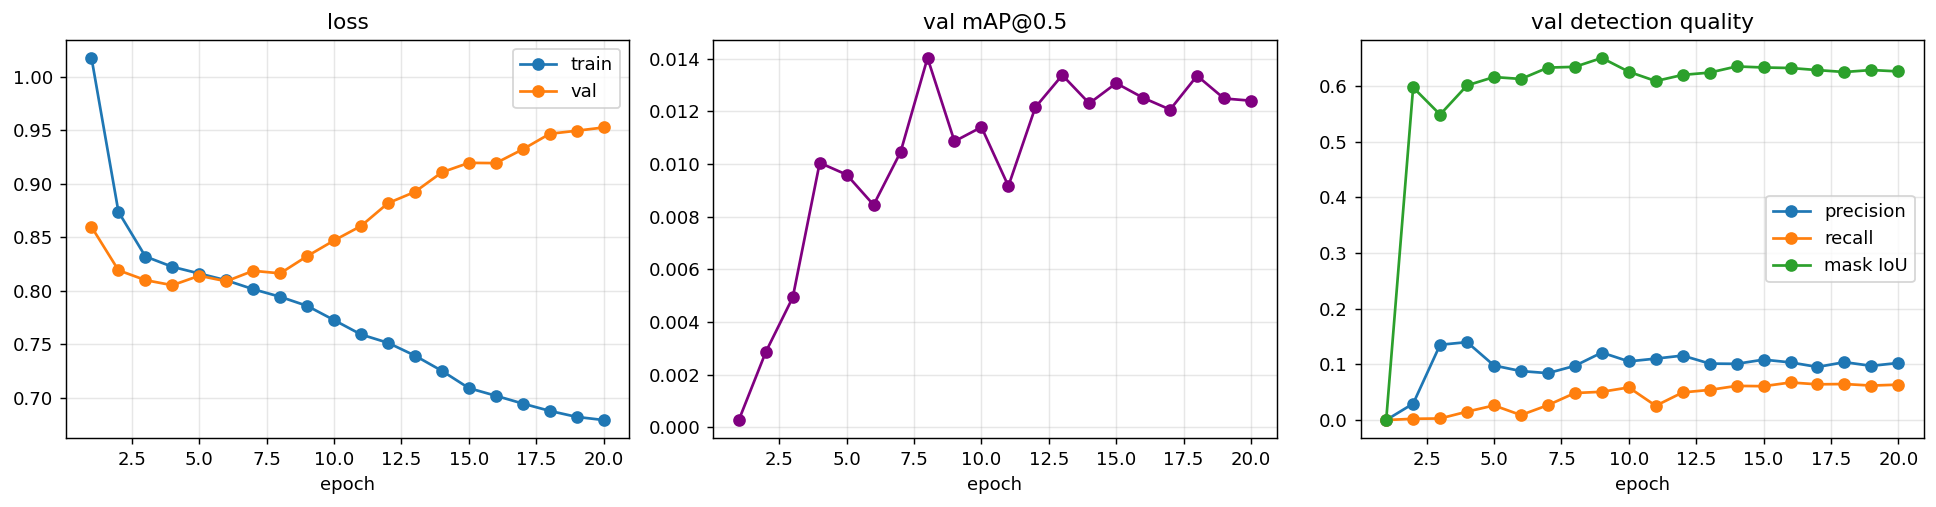
\includegraphics[width=\textwidth]{figures/training_curves.png}
\caption{Training history over $20$ epochs. \emph{Left:} train vs.\ validation
loss --- validation loss turns upward after $\sim\!4$ epochs, indicating
overfitting. \emph{Centre:} validation mAP@0.5, peaking near epoch~$8$.
\emph{Right:} detection quality --- mask IoU saturates early and high, while
precision and recall stay low. The decoupling of mask quality from detection
quality is the central result of this experiment.}
\label{fig:curves}
\end{figure*}

\begin{figure*}[p]
\centering
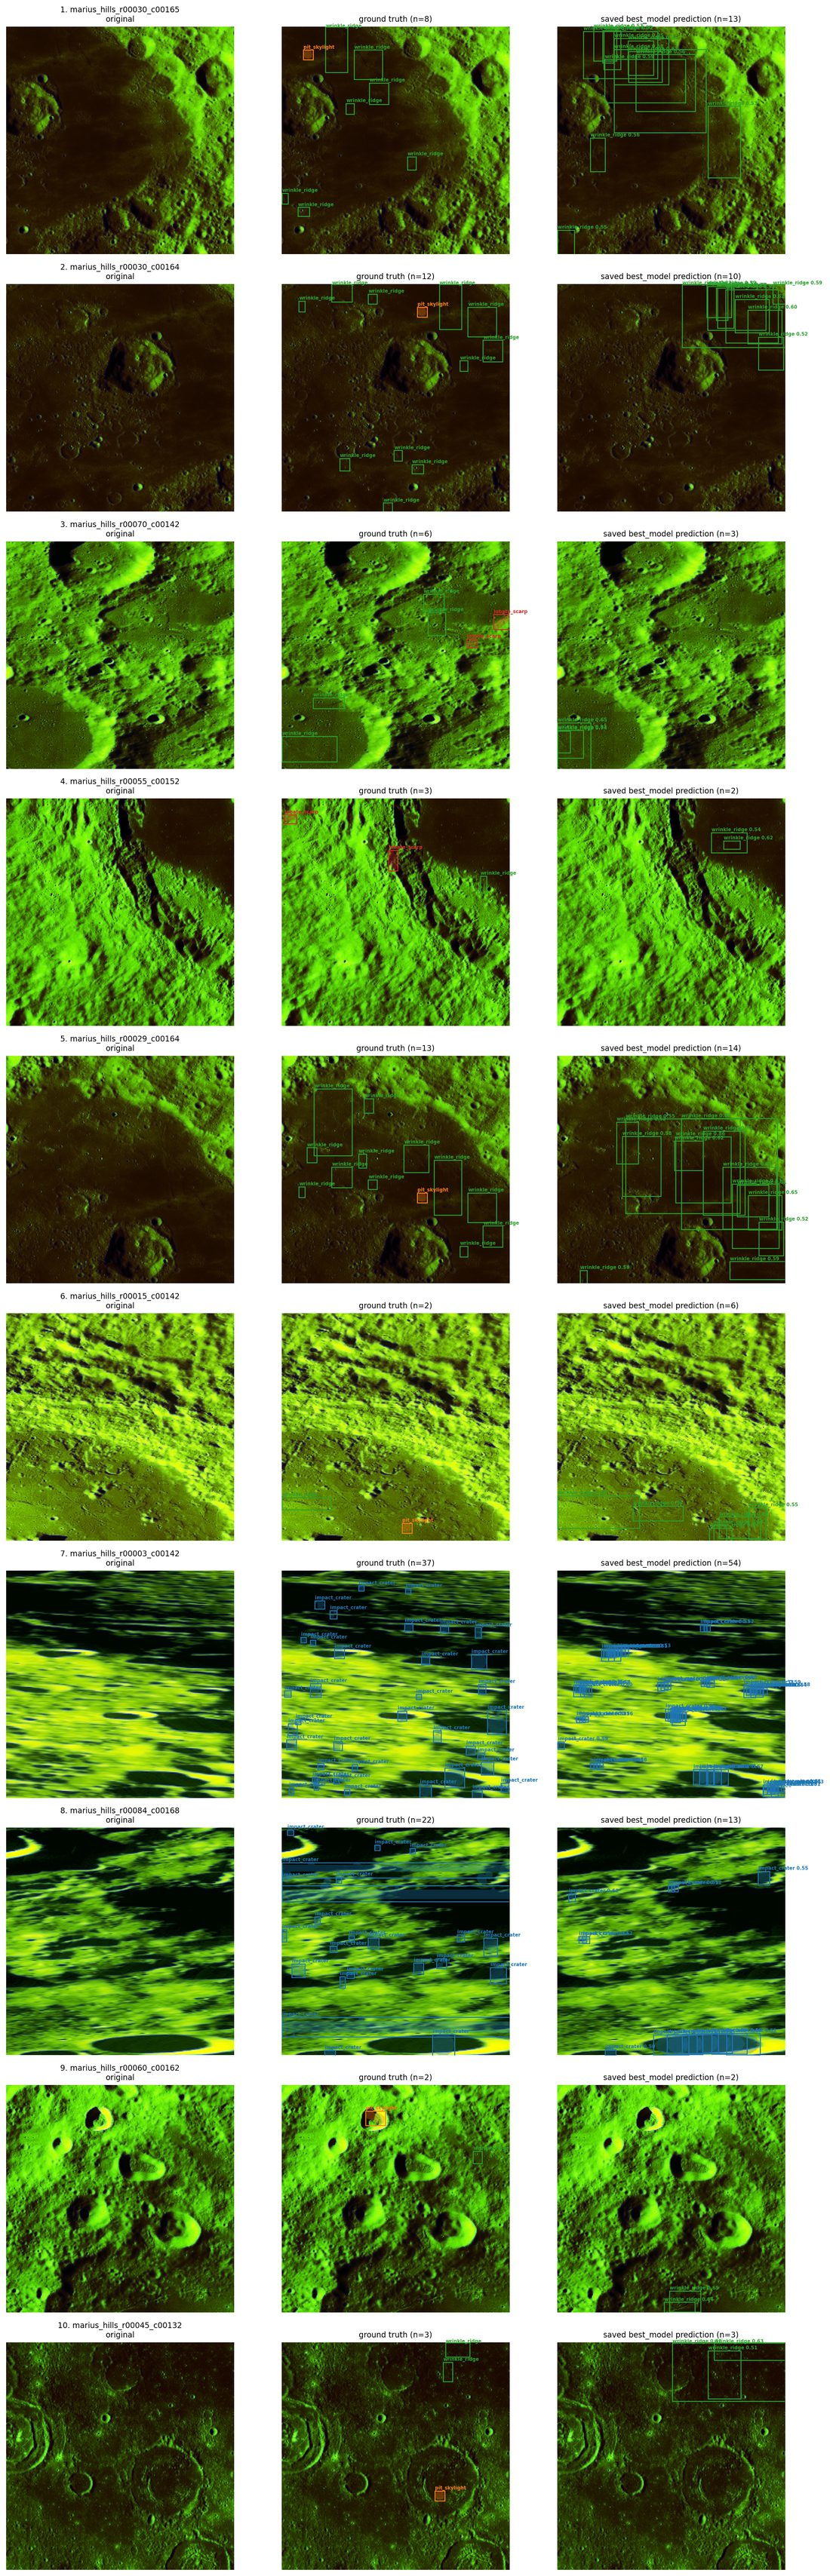
\includegraphics[height=0.92\textheight,keepaspectratio]{figures/prediction_samples.jpg}
\caption{Qualitative results on ten validation tiles from the Marius Hills region.
For each tile: original image (left), ground-truth instances (centre), and
model predictions with class and confidence (right). The network localises and
outlines the larger, higher-contrast craters and ridges reasonably well, but
misses faint or small features and is unreliable on the rare pit/skylight and
lobate-scarp classes.}
\label{fig:qual}
\end{figure*}

The qualitative panels in Fig.~\ref{fig:qual} are consistent with the numbers: on
tiles dominated by a few clear craters or a strong ridge the predictions line up
with the ground truth, but on busier or low-contrast tiles the model under-detects,
and the count error of $\sim\!6$ objects per tile reflects this systematic
shortfall.

\subsection{Challenges and lessons learned}
\label{sec:challenges}
Most of the effort in this part of the project went not into the network but into
the obstacles around it. They are listed roughly in order of how much they hurt the
final score.

\paragraph{Noisy semantic-to-instance conversion.}
The labels are semantic coverage masks, not object annotations. Connected-component
labelling turns them into instances, but it is a leaky abstraction: two touching
craters merge into one component, a single elongated ridge fragments into several,
and ``coverage-like'' channels produce blobs that are not really countable objects
at all. The area/shape filters and the $20\%$ coverage cut-off help, but the
supervision the detector sees is fundamentally noisier than in a hand-annotated
detection dataset, and that noise puts a ceiling on achievable precision.

\paragraph{Severe class imbalance and rarity.}
The classes that matter most scientifically are the rarest in the data. Lobate
scarps were too infrequent for the model to learn at all (AP $=0$), and
pit/skylights --- the whole motivation for the task --- appear so seldom that the
network almost never fires on them (AP $\approx 0.0003$). Frequency-based channel
selection keeps training stable, but it cannot manufacture positive examples that
are not there. This is the single biggest driver of the low mAP.

\paragraph{Small, low-contrast, scale-ambiguous features.}
Lunar features are small relative to the tile and often only marginally brighter or
darker than their surroundings, which is very different from the COCO objects the
backbone was pretrained on. Retuning the anchors to lunar scales ($8$--$128$\,px)
and keeping the native $256$\,px resolution both helped, but the domain gap between
natural RGB photographs and grayscale lunar terrain remains a real handicap for a
transfer-learned backbone.

\paragraph{Detection $\neq$ segmentation.}
The most instructive lesson is that good masks did not buy good detections. Mask
IoU/Dice are high precisely because they are only measured on objects that were
already matched; the bottleneck is upstream, in the proposal and box stage actually
finding and correctly classifying the regions. Improving the mask head further would
not move the headline metric --- the next gains have to come from recall.

\paragraph{Overfitting on limited positives.}
With relatively few labelled positives, the model began overfitting after only a
handful of epochs. Dropout, weight decay and augmentation
slowed it but did not prevent it; more aggressive augmentation, class-balanced
sampling, or simply more labelled data would likely help more than a bigger network.

\paragraph{Compute budget.}
Training on CPU made every experiment expensive --- roughly half a day per full run
--- which is why the loop was engineered to be resumable and why hyper-parameter
exploration was necessarily limited. Most of the design choices above were made to
get the most out of a single, long, interruptible run rather than many short ones.

\paragraph{What would change next.}
Given more time the next steps would be to (i) address the imbalance directly with
class-balanced or hard-negative sampling and a focal-style loss; (ii) treat the rare
pit/skylight class as a dedicated detection problem rather than one head among four;
(iii) move to GPU so the schedule can be tuned and stopped at the validation-loss
minimum; and (iv) revisit the instance-generation step, since cleaner targets would
raise the ceiling on everything downstream.

\subsection{Conclusions}
\label{sec:conclusions}
Mask R-CNN was adapted to instance-segment four classes of lunar features from
Marius Hills tiles, contributing a channel-audited semantic-to-instance pipeline, a
deeper custom box and residual mask head, and lunar-scale anchors, all trained in a
crash-safe CPU loop. The model learns to outline features well (mask IoU $0.64$,
Dice $0.77$) but detects them poorly (mAP@0.5 $\approx 1\%$), with the rare and
most interesting classes essentially undetected. The clear separation between mask
quality and detection quality, and the data-side reasons behind it, are the main
takeaways and the right starting point for the next iteration.

\section{Lunar Surface Feature Segmentation}
\label{sec:moon_recognition}

\subsection{Motivation and Task Definition}
\label{sec:mr_motivation}

Complementing the instance-segmentation approach of the previous section, which detects individual feature objects, we now address the same Marius Hills terrain as a dense, pixel-level labelling problem. We frame the task as \textit{multi-label semantic segmentation}: given a grayscale image patch of the lunar surface, predict, at the pixel level, which of seven geomorphological feature classes are present. Such pixel-level maps are a prerequisite for mission planning, geological analysis, and the identification of scientifically valuable sites such as lava-tube skylights and impact craters, while avoiding the inconsistency of manually cataloguing the high-resolution imagery returned by the Lunar Reconnaissance Orbiter (LRO).

The seven target classes are:
\begin{enumerate}
    \item \texttt{impact\_crater} --- circular depressions formed by hypervelocity impacts,
    \item \texttt{pit\_skylight} --- openings into subsurface lava tubes,
    \item \texttt{wrinkle\_ridge} --- compressional tectonic folds in mare basalts,
    \item \texttt{lobate\_scarp} --- cliff-like fault scarps formed by global contraction,
    \item \texttt{irregular\_mare\_patch} --- inhomogeneous mare volcanic units,
    \item \texttt{apollo\_site} --- Apollo mission landing sites,
    \item \texttt{candidate\_rille} --- linear depressions of volcanic or tectonic origin.
\end{enumerate}

\noindent
Because multiple classes can coexist in a single pixel (e.g.\ a pit on the rim of a crater), this is posed as independent binary classification per class rather than a single-label softmax problem.

\subsection{Dataset}
\label{sec:mr_dataset}

\paragraph{Imagery.}
Training data consists of Wide Angle Camera (WAC) grayscale tiles downloaded from the LROC archive, covering the \textit{Marius Hills} volcanic region on the Oceanus Procellarum --- a site of particular scientific interest due to its high density of pit skylights, wrinkle ridges, and rilles.

\paragraph{Tiling.}
The raw raster is divided into overlapping training patches using a sliding-window tiler:
\begin{itemize}
    \item Tile size: $256 \times 256$ pixels,
    \item Stride: $128$ pixels (50\% overlap between adjacent tiles),
    \item Tiles with no labelled features are kept with probability $p=0.1$ to maintain background examples,
    \item Total tiles produced: 15{,}931.
\end{itemize}

\paragraph{Labels.}
Ground-truth annotations are sourced from the LROC feature catalogue (shapefiles and CSV), rasterised onto the tile grid as binary masks. To account for the point-like or line-like nature of some classes, morphological dilation is applied per class after rasterisation:
\begin{itemize}
    \item \texttt{pit\_skylight}, \texttt{apollo\_site}, \texttt{irregular\_mare\_patch}: disk kernel of radius 5,
    \item \texttt{wrinkle\_ridge}, \texttt{lobate\_scarp}: disk kernel of radius 3 (linear features),
    \item \texttt{candidate\_rille}: disk kernel of radius 2,
    \item \texttt{impact\_crater}: no dilation (already area features).
\end{itemize}

\paragraph{Train / validation split.}
Tiles are split 80/20 by random permutation with a fixed seed (42), yielding 12{,}745 training tiles and 3{,}186 validation tiles; the same split is reused across all configurations so that comparisons between models are paired.

\paragraph{Label prevalence and channel saturation.}
Table~\ref{tab:prevalence} reports the exact fraction of positive pixels per class, computed over all 15{,}931 tiles. The imbalance is extreme \emph{in both directions}: the \texttt{impact\_crater} channel covers 82.1\% of all pixels --- half of the tiles are \emph{entirely} positive --- while the five rarest classes have prevalences below $1.4\times10^{-4}$. The crater channel therefore behaves closer to a coverage-like layer than to a sparse target feature, a possibility explicitly flagged in the course material. This has a direct consequence for interpretation: the Average Precision of an uninformative predictor equals the class prevalence, so per-class AP values must be read against the baselines in Table~\ref{tab:prevalence} rather than against zero.

\begin{table}[htbp]
\centering
\caption{Per-class positive-pixel prevalence over the full dataset (15{,}931 tiles, $1.04\times10^9$ pixels per channel). The prevalence is also the AP of an uninformative (chance-level) predictor for that class.}
\label{tab:prevalence}
\resizebox{\columnwidth}{!}{%
\begin{tabular}{lrr}
\toprule
Class & Prevalence & Tiles fully covered \\
\midrule
\texttt{impact\_crater}        & $8.21\times10^{-1}$ & 50.7\% \\
\texttt{wrinkle\_ridge}        & $6.38\times10^{-3}$ & 0 \\
\texttt{lobate\_scarp}         & $1.34\times10^{-4}$ & 0 \\
\texttt{pit\_skylight}         & $4.2\times10^{-5}$  & 0 \\
\texttt{irregular\_mare\_patch} & $2.0\times10^{-5}$  & 0 \\
\texttt{apollo\_site}          & $1.5\times10^{-5}$  & 0 \\
\texttt{candidate\_rille}      & $1.0\times10^{-5}$  & 0 \\
\bottomrule
\end{tabular}
}
\end{table}

\paragraph{Limitation: spatial overlap between splits.}
Because adjacent tiles overlap by 50\%, a random tile-level split leaks pixels between the two sets: we measured that \emph{every} validation tile overlaps at least one training tile. Absolute validation scores are therefore optimistic (they partially reward memorisation of seen pixels), although \emph{relative} comparisons between configurations trained and evaluated on the identical split remain informative. A leakage-free \emph{spatial block split} (contiguous $1024$-px blocks assigned to validation, with overlapping boundary tiles discarded from training) has been implemented in \texttt{data/splits.py}; its impact is discussed where relevant, in particular for the augmentation study (Sec.~\ref{sec:mr_augmentation}).

\subsection{Input Pre-processing Pipeline}
\label{sec:mr_preprocessing}

Each grayscale tile is converted into a three-channel tensor to provide the network with complementary representations of the same image:

\begin{enumerate}
    \item \textbf{Normalised intensity}: min-max normalisation of the raw pixel values to $[0,1]$.
    \item \textbf{CLAHE}: Contrast Limited Adaptive Histogram Equalization (\texttt{skimage.exposure.equalize\_adapthist}, clip limit $0.03$, default kernel of $1/8$ of the image side) to enhance local contrast and make faint features more visible.
    \item \textbf{Sobel edges}: magnitude of the Sobel gradient computed on the normalised tile, highlighting boundaries and ridge-like structures.
\end{enumerate}

\noindent
Because CLAHE is computationally expensive (${\sim}3$ s per tile on CPU), a one-time precomputation step caches all three-channel tensors as compressed \texttt{.npz} files. During training and inference, tiles are loaded from cache, eliminating the CLAHE bottleneck from the data pipeline.

\subsection{Model Architecture: SmallUNet}
\label{sec:mr_architecture}

The model follows the U-Net encoder-decoder paradigm~\cite{ronneberger2015unet} with modifications designed to reduce parameter count while preserving multi-scale feature reuse.

\paragraph{Encoder.}
Three successive \textit{Down} blocks, each consisting of $2\times 2$ max-pooling followed by a \textit{DoubleConv} block. A DoubleConv block applies two consecutive $3\times 3$ convolution $\to$ BatchNorm $\to$ ReLU operations.

\paragraph{Decoder.}
Three symmetric \textit{Up} blocks, each using transposed convolution for $2\times$ upsampling, concatenation with the corresponding encoder skip connection, and a DoubleConv block. Odd-dimension padding ensures spatial alignment between encoder and decoder feature maps.

\paragraph{Output head.}
A $1\times 1$ convolution maps the final feature map (32 channels) to 7 independent logit channels. Binary sigmoid is applied per channel at inference time to produce class probability maps.

\paragraph{Optional residual shortcuts.}
Each DoubleConv block can optionally include a residual (ResNet-style) shortcut: the block input is added to the post-convolution output before the final ReLU, with a $1\times 1$ projection convolution when channel dimensions differ. This improves gradient flow and slightly increases parameter count.

\paragraph{Bottleneck dropout.}
Spatial Dropout2d can be applied at the bottleneck (deepest encoder level) to regularise the model when training labels are sparse.

The spatial flow of the network with base width $w=32$ and $256\times 256$ input is:

\[
\begin{array}{c}
(3,\,256,256)
\xrightarrow{\text{inc}}   (32,\,256,256)\\[2pt]
\xrightarrow{\text{down}_1}(64,\,128,128)\\[2pt]
\xrightarrow{\text{down}_2}(128,\,64,64)\\[2pt]
\xrightarrow{\text{down}_3}(256,\,32,32)\\[4pt]
\xrightarrow{\text{up}_1}  (128,\,64,64)\\[2pt]
\xrightarrow{\text{up}_2}  (64,\,128,128)\\[2pt]
\xrightarrow{\text{up}_3}  (32,\,256,256)\\[2pt]
\xrightarrow{\text{out}}   (7,\,256,256)
\end{array}
\]

\noindent
The base width $w$ is configurable; doubling $w$ quadruples the parameter count. The three widths explored in this work are summarised in Table~\ref{tab:bw_params}.

\begin{table}[htbp]
\centering
\caption{Parameter counts for each base width.}
\label{tab:bw_params}
\begin{tabular}{lrr}
\toprule
Base width $w$ & Channel progression & Parameters \\
\midrule
16 & 16--32--64--128  &    505{,}095 \\
32 & 32--64--128--256 & 2{,}014{,}727 \\
64 & 64--128--256--512 & 8{,}047{,}623 \\
\bottomrule
\end{tabular}
\end{table}

\subsection{Loss Functions}
\label{sec:mr_loss}

Two composite loss functions are compared.

\paragraph{BCEDiceLoss.}
Binary cross-entropy summed with a soft Dice loss, averaged across classes:
\[
\mathcal{L}_{\text{BCEDice}} = \mathcal{L}_{\text{BCE}} + \mathcal{L}_{\text{Dice}},
\]
\[
\mathcal{L}_{\text{Dice}} = 1 - \frac{1}{C}\sum_{c=1}^{C} \frac{2\sum_i p_i^c\, y_i^c + \varepsilon}{\sum_i p_i^c + \sum_i y_i^c + \varepsilon}
\]
where $p_i^c$ is the predicted probability and $y_i^c$ the ground-truth label for pixel $i$ and class $c$, and $\varepsilon=10^{-6}$ ensures numerical stability.

\paragraph{FocalDiceLoss.}
Replaces the BCE term with the binary focal loss~\cite{lin2017focal} to down-weight easy negatives and focus training on hard positives, a natural choice for class-imbalanced segmentation:
\[
\mathcal{L}_{\text{focal}}(p,y) = -\alpha\,y\,(1-p)^\gamma \log p
                                   -(1-\alpha)(1-y)\,p^\gamma \log(1-p)
\]
with $\gamma=2$ and $\alpha=0.25$. The Dice term additionally uses per-class weights $\mathbf{w} = [1.0,\,4.0,\,5.0,\,5.0,\,5.0,\,5.0,\,5.0]$ to penalise misdetection of rare classes more heavily:
\[
\mathcal{L}_{\text{FocalDice}} = \mathcal{L}_{\text{focal}} + \sum_{c=1}^{C} w_c \,\mathcal{L}_{\text{Dice}}^c
\]

\subsection{Training Protocol}
\label{sec:mr_training}

All definitive experiments were run on a \textbf{NVIDIA Tesla T4} (16 GB VRAM) via the CloudVeneto HPC facility, using the full training dataset of 15{,}931 tiles for 30 epochs. The local MPS (Apple Silicon) runs at 4{,}000 tiles / 20 epochs served as rapid prototyping before the full runs.

\begin{itemize}
    \item Batch size: 16 (T4) / 8 (MPS),
    \item Optimizer: Adam,
    \item Learning rate schedule: cosine annealing, $\eta_{\max}=10^{-3}$, $\eta_{\min}=10^{-5}$, $T_{\max}=30$,
    \item No gradient clipping (the trainer supports it, but it was disabled in all runs: \texttt{clip\_grad\_norm\_} forces a CPU synchronisation per batch on MPS),
    \item Checkpoints saved at end of training for each experimental configuration.
\end{itemize}

\paragraph{Metrics.}
Validation is performed after every epoch. For each class $c$ and a fixed threshold $\tau=0.5$ we compute precision, recall, F1, and Intersection over Union (IoU). Additionally, \textit{Average Precision} (AP) is computed as the area under the precision-recall curve (threshold-free), using \texttt{sklearn.metrics.average\_precision\_score}. Aggregate metrics are macro-averages across the seven classes.

\subsection{Study 1 --- Architecture Ablation}
\label{sec:mr_arch_ablation}

Five configurations are compared in a cumulative fashion, each adding one component to the previous best:

\begin{enumerate}
    \item \textbf{BCEDice}: plain DoubleConv blocks, BCEDiceLoss --- the reference baseline.
    \item \textbf{FocalDice}: same architecture, FocalDiceLoss with class weights.
    \item \textbf{+residual}: FocalDice + residual shortcuts inside DoubleConv blocks.
    \item \textbf{+dropout}: FocalDice + bottleneck Dropout2d($p=0.3$).
    \item \textbf{+both}: FocalDice + residual + dropout.
\end{enumerate}

Table~\ref{tab:arch_comparison} reports the full-run results (15{,}931 tiles, 30 epochs, T4).
Figure~\ref{fig:arch_metrics} shows the per-class validation curves.

\begin{table}[htbp]
\centering
\caption{Architecture ablation on the full dataset (Tesla T4, 30 epochs). Metrics are macro-averaged across the seven classes. Crater AP and Ridge AP are single-class AP values for \texttt{impact\_crater} and \texttt{wrinkle\_ridge}, which span the performance range.}
\label{tab:arch_comparison}
\resizebox{\columnwidth}{!}{%
\begin{tabular}{lrrrrrrr}
\toprule
Config & Params & Epoch (s) & Final loss & Mean F1 & Mean IoU & Mean AP & Ridge AP \\
\midrule
BCEDice    & 1{,}927{,}207 & 208 & 0.876 & 0.1998 & 0.1666 & 0.1989 & 0.440 \\
FocalDice  & 1{,}927{,}207 & 214 & 3.893 & 0.1994 & 0.1632 & 0.1945 & 0.417 \\
+residual  & 2{,}014{,}727 & 257 & 3.873 & 0.2065 & 0.1675 & 0.1995 & 0.443 \\
+dropout   & 1{,}927{,}207 & 215 & 3.894 & 0.2018 & 0.1643 & 0.1938 & 0.405 \\
\textbf{+both} & \textbf{2{,}014{,}727} & 258 & \textbf{3.863} & \textbf{0.2076} & \textbf{0.1688} & \textbf{0.2004} & \textbf{0.453} \\
\bottomrule
\end{tabular}
}
\end{table}

\begin{figure}[htbp!]
\centering
\begin{subfigure}[b]{0.32\textwidth}
    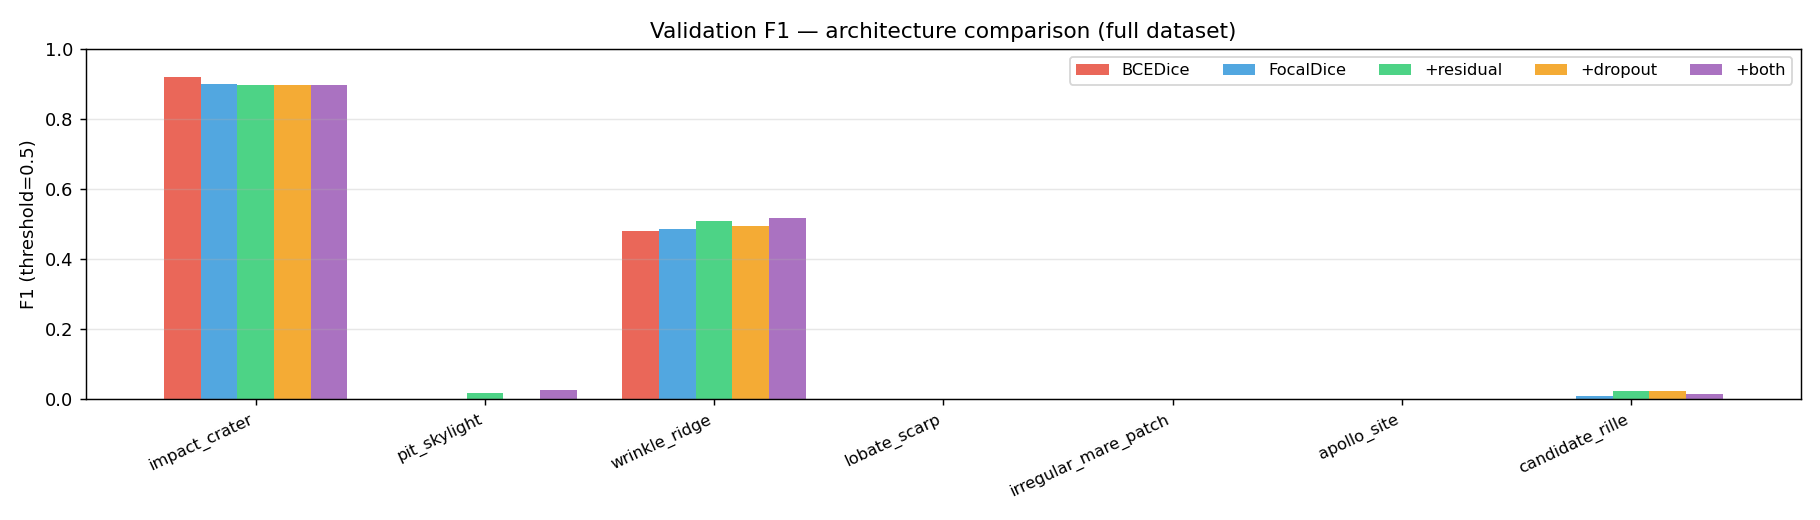
\includegraphics[width=\textwidth]{figures/MR/cloudveneto_arch_val_f1.png}
    \caption{Validation F1}
\end{subfigure}
\hfill
\begin{subfigure}[b]{0.32\textwidth}
    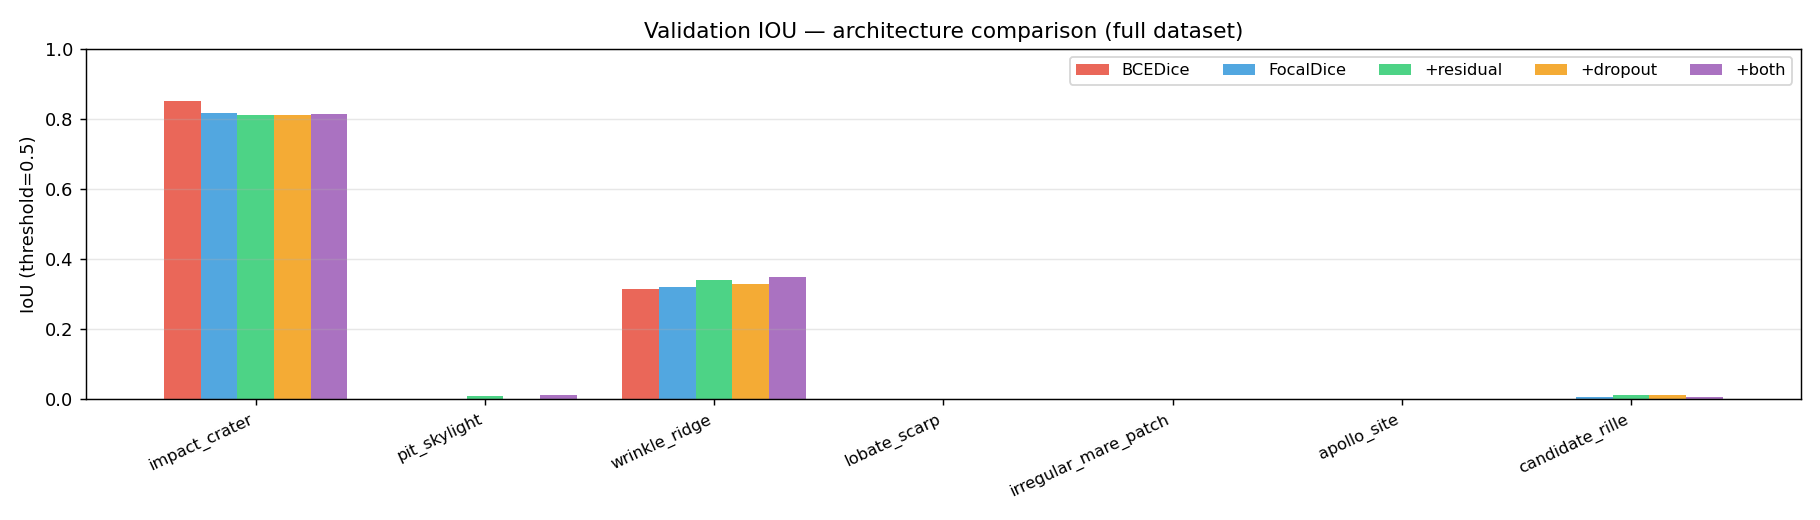
\includegraphics[width=\textwidth]{figures/MR/cloudveneto_arch_val_iou.png}
    \caption{Validation IoU}
\end{subfigure}
\hfill
\begin{subfigure}[b]{0.32\textwidth}
    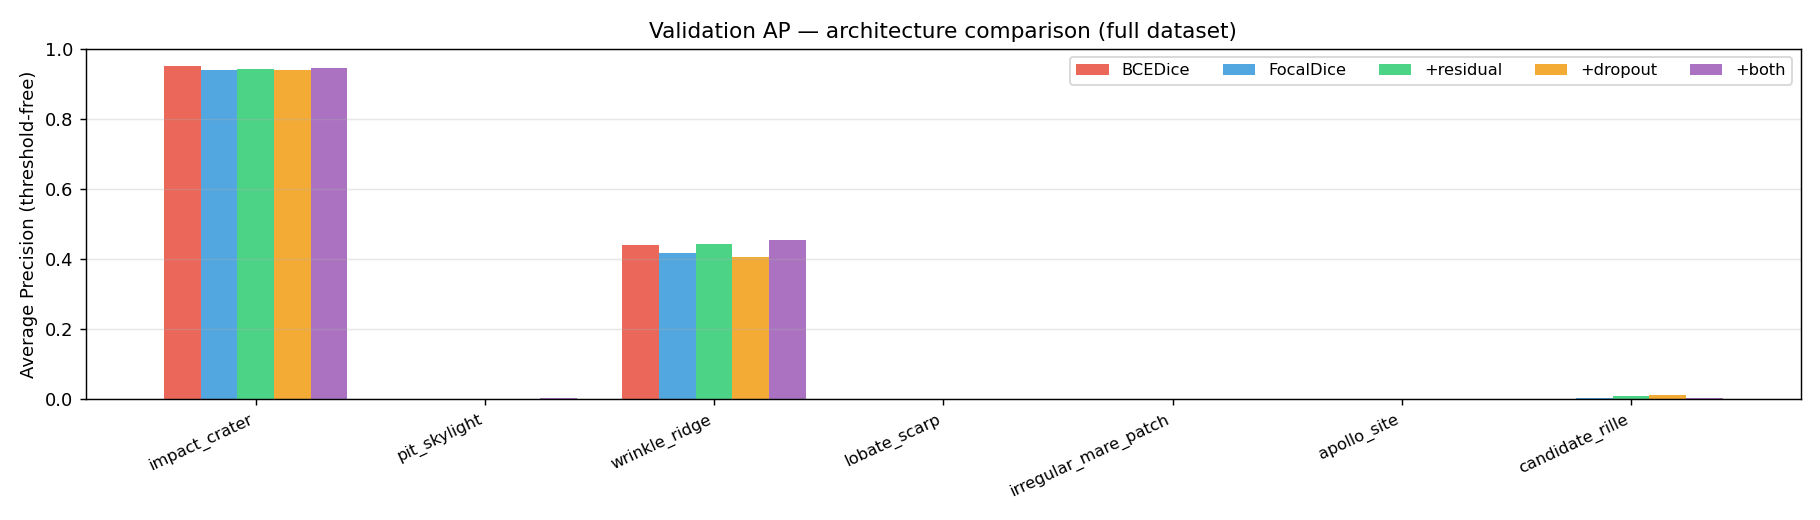
\includegraphics[width=\textwidth]{figures/MR/cloudveneto_arch_val_ap.png}
    \caption{Validation AP}
\end{subfigure}
\caption{Per-class validation metrics across training epochs for the five architecture configurations (full T4 run, 30 epochs). \textbf{+both} (residual + dropout + FocalDice) achieves the highest aggregate performance on all three metrics.}
\label{fig:arch_metrics}
\end{figure}

\paragraph{Key findings.}
Residual shortcuts consistently improve over the plain DoubleConv baseline on aggregate F1, IoU, and AP (+residual vs FocalDice: $+0.0071$ mean F1, $+0.0050$ mean AP). Dropout alone does not help --- it degrades both mean AP and ridge AP relative to plain FocalDice, likely because sparse labels already act as a strong regulariser. The combination \textbf{+both} achieves the best mean F1 (0.2076), best mean IoU (0.1688), and best mean AP (0.2004), as well as the highest ridge AP (0.453). Impact-crater AP is uniformly high (0.939--0.951) across all configurations, but given the 0.821 prevalence baseline (Table~\ref{tab:prevalence}) this represents only a modest lift over chance; the architecture choice matters primarily for rare and structurally subtle classes such as ridges, where AP~0.44--0.45 is ${\sim}70\times$ the 0.0064 chance level.

\subsection{Study 2 --- Network Width}
\label{sec:mr_width}

Using the best architecture from Study~1 (\textbf{+both}: FocalDice + residual + dropout=0.3), we sweep the base width $w \in \{16, 32, 64\}$, corresponding to 505K, 2.0M, and 8.0M parameters respectively.

\begin{table}[htbp]
\centering
\caption{Base-width sweep (FocalDice + residual + dropout=0.3, full T4 run, 30 epochs).}
\label{tab:bw_comparison}
\resizebox{\columnwidth}{!}{%
\begin{tabular}{lrrrrrr}
\toprule
Config & Params & Epoch (s) & Mean F1 & Mean IoU & Mean AP & Ridge AP \\
\midrule
small ($w=16$)   &    505{,}095 &  139 & 0.2031 & 0.1665 & 0.2003 & 0.451 \\
default ($w=32$) & 2{,}014{,}727 &  258 & 0.2093 & 0.1704 & 0.2010 & 0.456 \\
wide ($w=64$)    & 8{,}047{,}623 &  582 & \textbf{0.2153} & \textbf{0.1733} & \textbf{0.2016} & 0.445 \\
\bottomrule
\end{tabular}
}
\end{table}

\begin{figure}[htbp!]
\centering
\begin{subfigure}[b]{0.32\textwidth}
    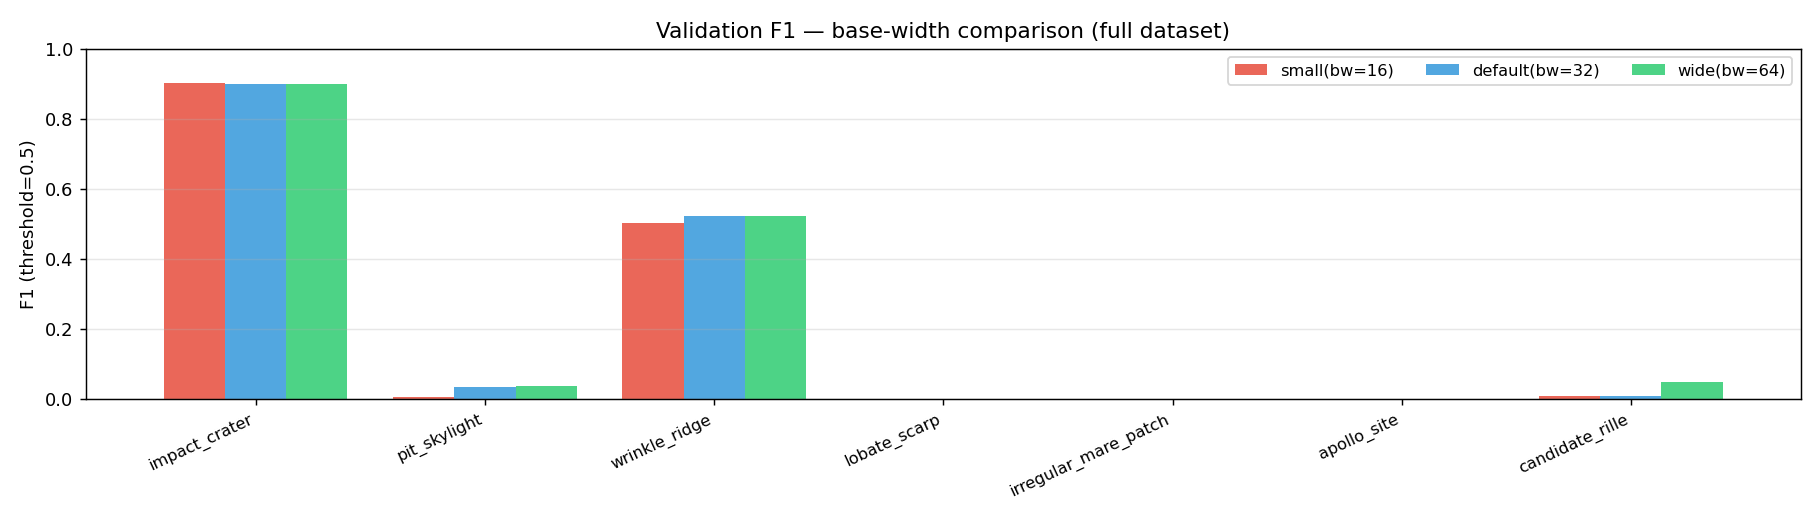
\includegraphics[width=\textwidth]{figures/MR/cloudveneto_bw_val_f1.png}
    \caption{Validation F1}
\end{subfigure}
\hfill
\begin{subfigure}[b]{0.32\textwidth}
    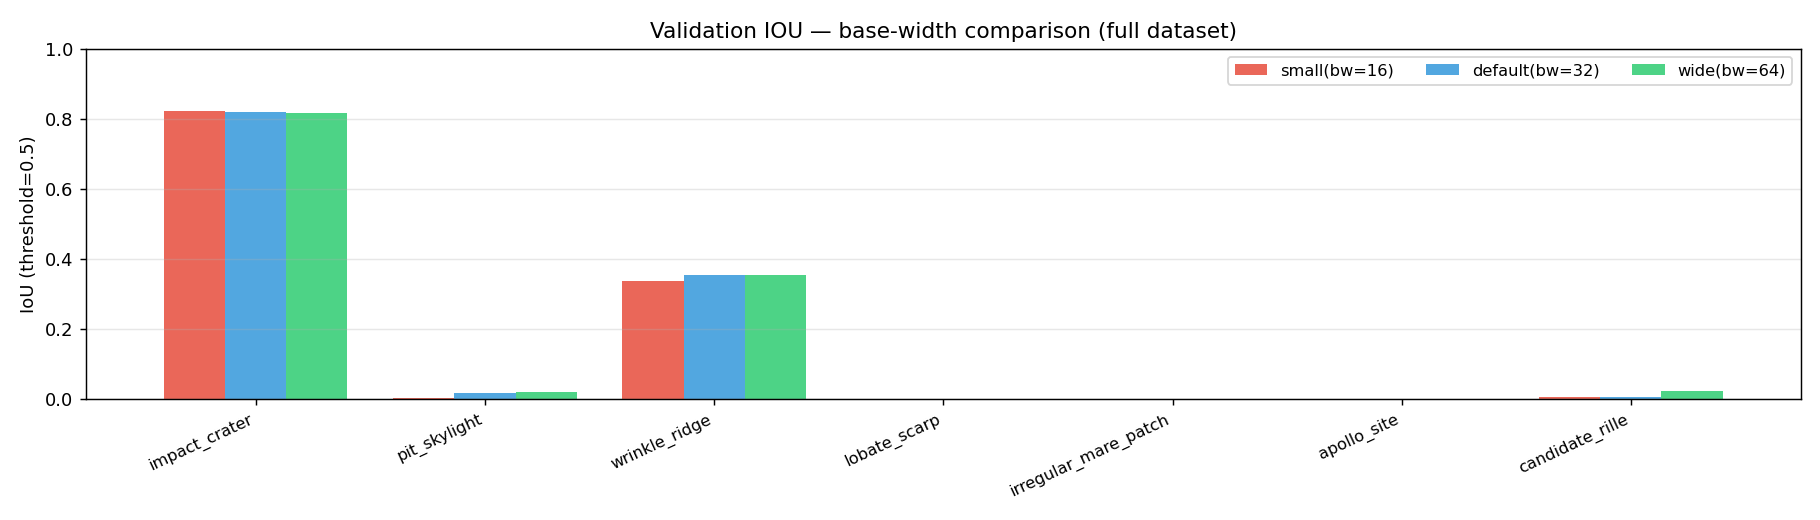
\includegraphics[width=\textwidth]{figures/MR/cloudveneto_bw_val_iou.png}
    \caption{Validation IoU}
\end{subfigure}
\hfill
\begin{subfigure}[b]{0.32\textwidth}
    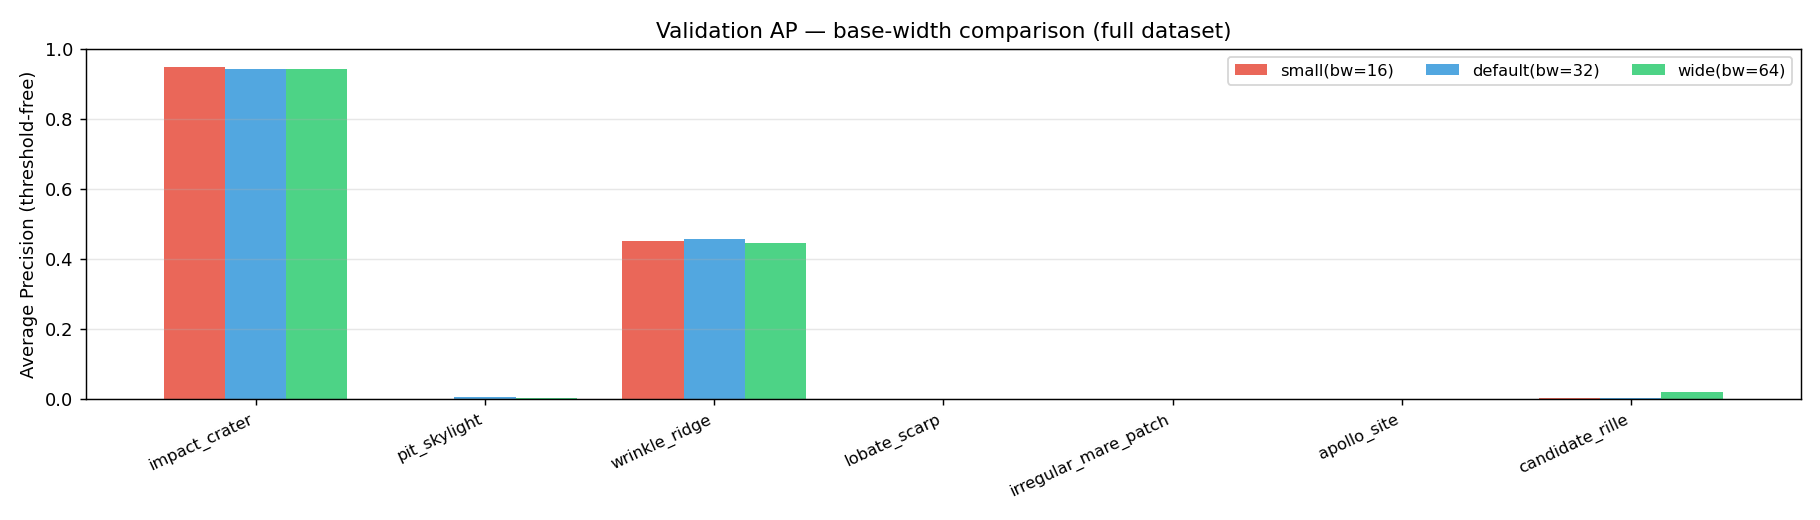
\includegraphics[width=\textwidth]{figures/MR/cloudveneto_bw_val_ap.png}
    \caption{Validation AP}
\end{subfigure}
\caption{Validation metrics for three network widths (full T4 run, 30 epochs). Wider networks achieve marginally higher scores but exhibit severely diminishing returns in terms of parameters and training time.}
\label{fig:bw_metrics}
\end{figure}

\paragraph{Key findings.}
The wide model ($w=64$) achieves the best mean AP (0.2016) and mean F1 (0.2153), but the improvement over the default ($w=32$) is marginal: $+0.0006$ mean AP, $+0.006$ mean F1, at the cost of a 4$\times$ parameter increase and a ${\sim}2.3\times$ increase in training time per epoch (258 s $\to$ 582 s). Strikingly, the small model ($w=16$) with only 505K parameters achieves a mean AP of 0.2003 --- within 0.001 of the 8M-parameter wide model --- making it the most parameter-efficient option. For deployment on resource-constrained hardware the small model offers the best trade-off.

\subsection{Study 3 --- Data Augmentation}
\label{sec:mr_augmentation}

Using \textbf{+both} at $w=32$, we isolate the effect of geometric augmentation. The augmented pipeline applies random horizontal and vertical flips and 90\degree/180\degree/270\degree rotations to training tiles. No augmentation is applied to validation.

\begin{table}[htbp]
\centering
\caption{Augmentation study (FocalDice + residual + dropout=0.3, $w=32$, full T4 run, 30 epochs). Crater AP is given for reference; Ridge AP highlights the most affected rare class.}
\label{tab:aug_comparison}
\resizebox{\columnwidth}{!}{%
\begin{tabular}{lrrrrrr}
\toprule
Config & Final loss & Mean F1 & Mean IoU & Mean AP & Crater AP & Ridge AP \\
\midrule
\textbf{no augmentation} & \textbf{3.698} & \textbf{0.2986} & \textbf{0.2289} & \textbf{0.2647} & \textbf{0.947} & \textbf{0.558} \\
+augmentation            &        3.863  &        0.2124  &        0.1724  &        0.2027  &        0.942  &        0.457  \\
\bottomrule
\end{tabular}
}
\end{table}

\begin{figure}[htbp!]
\centering
\begin{subfigure}[b]{0.32\textwidth}
    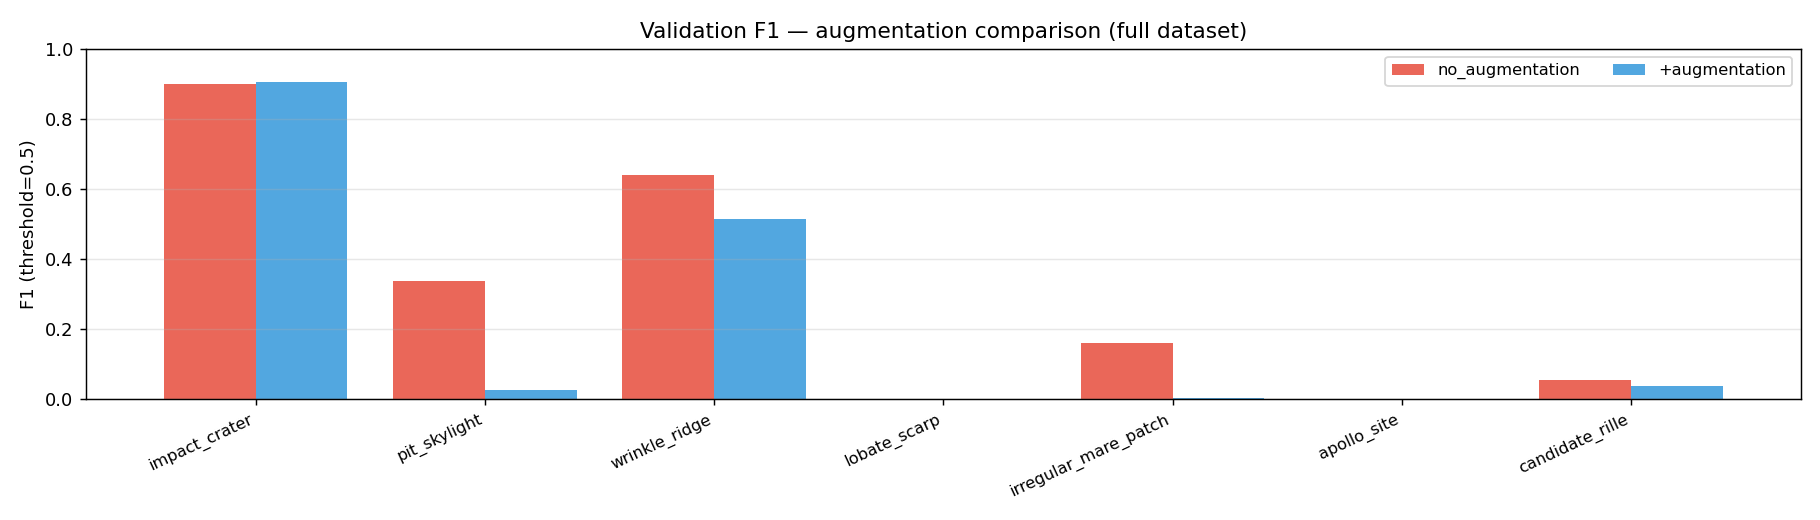
\includegraphics[width=\textwidth]{figures/MR/cloudveneto_aug_val_f1.png}
    \caption{Validation F1}
\end{subfigure}
\hfill
\begin{subfigure}[b]{0.32\textwidth}
    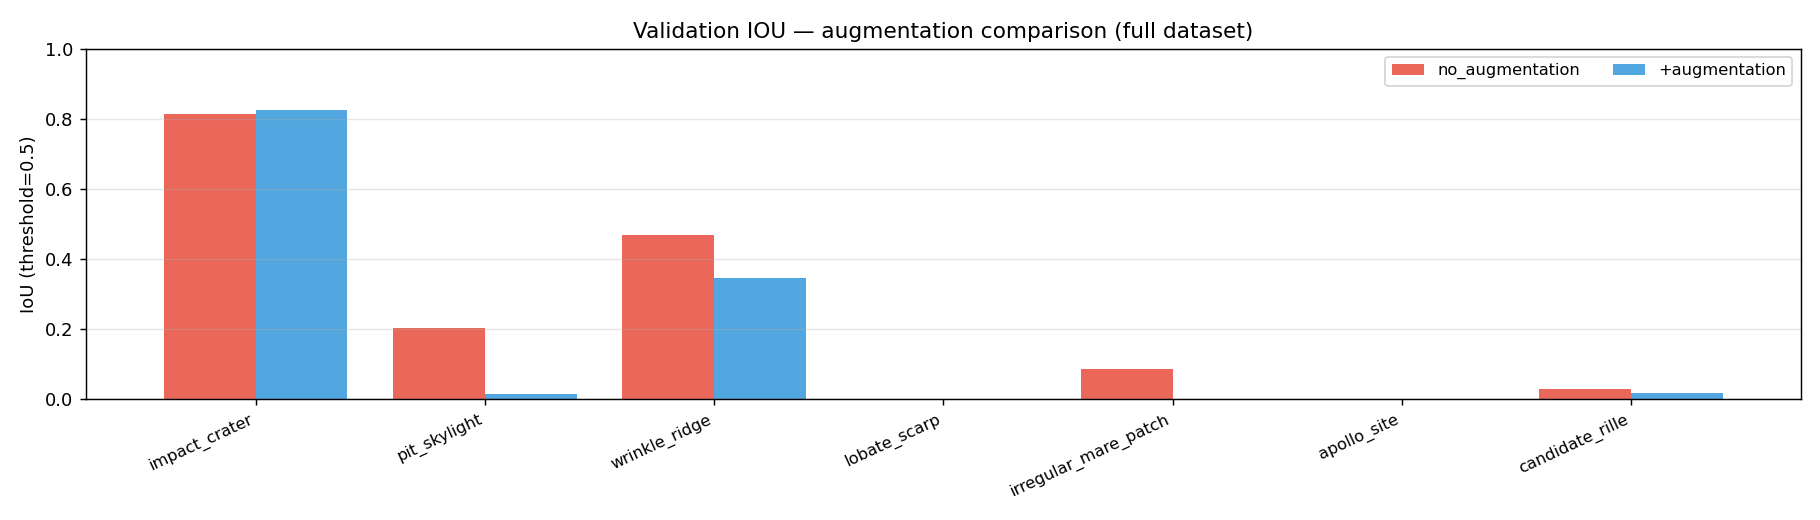
\includegraphics[width=\textwidth]{figures/MR/cloudveneto_aug_val_iou.png}
    \caption{Validation IoU}
\end{subfigure}
\hfill
\begin{subfigure}[b]{0.32\textwidth}
    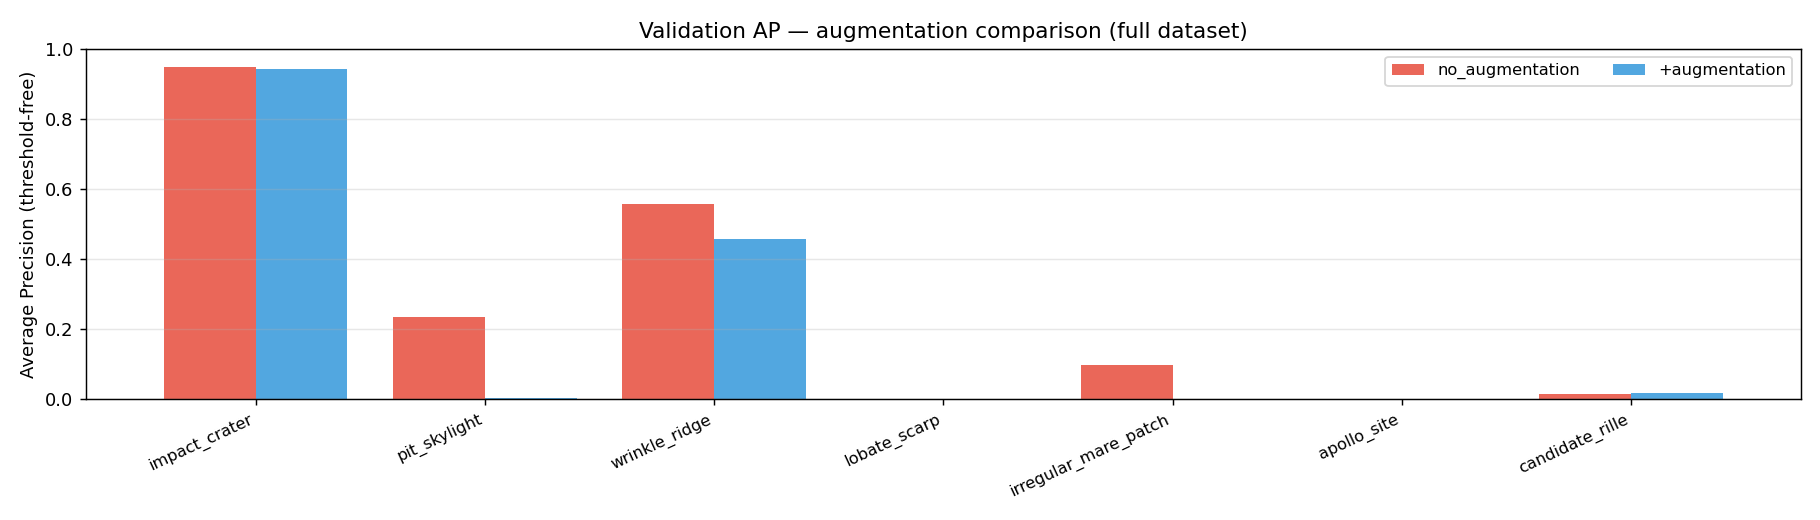
\includegraphics[width=\textwidth]{figures/MR/cloudveneto_aug_val_ap.png}
    \caption{Validation AP}
\end{subfigure}
\caption{Validation metrics with and without geometric augmentation (full T4 run, 30 epochs). No augmentation outperforms the augmented training on all metrics.}
\label{fig:aug_metrics}
\end{figure}

\paragraph{Key findings.}
This is the most striking result of the ablation campaign. Training without augmentation produces a model that is dramatically better on every metric: mean F1 improves by 0.086 (40\% relative), mean AP improves by 0.062 (31\% relative), and ridge AP improves from 0.457 to 0.558 (22\% relative).

Two effects plausibly combine to produce this result, and the present experiment cannot fully separate them.

First, a \emph{geological} effect: the Marius Hills region has a strong directional bias --- wrinkle ridges run predominantly in a narrow range of orientations dictated by the regional stress field, and rilles follow the same orientation. Moreover, the Sun azimuth is consistent within the WAC mosaic, so flips and $90\degree$ rotations also produce illumination directions that never occur in the data. Applying such transforms presents the model with feature orientations and shading that are physically absent in the training region, injecting false diversity. Generic augmentation implicitly assumes that the transformed inputs remain representative of the target distribution~\cite{shorten2019augmentation}, an assumption violated here. Impact craters, being rotationally symmetric, are unaffected, which explains why crater AP is nearly identical in both conditions (0.947 vs 0.942).

Second, a \emph{methodological} confound: as noted in Sec.~\ref{sec:mr_dataset}, the random tile split leaks overlapping pixels into validation. A model trained without augmentation is freer to memorise tile appearance and is rewarded for it on a leaky split, while augmentation suppresses exactly this memorisation. Part of the measured gap could therefore be an artefact of the split rather than a property of the data. To separate the two effects, the comparison was re-run under the leakage-free spatial block split.

\paragraph{Leakage-free re-run.}
The augmentation pair was re-trained with \texttt{spatial\_train\_val\_split}: both arms share an identical pixel-disjoint split, the same initialisation seed, and the same cosine schedule, so the \emph{only} difference between them is augmentation. The re-run used a scaled paired protocol on local hardware (10{,}000 tiles, 30 epochs; a paired comparison remains internally valid at reduced scale), with a smaller 6{,}000-tile/15-epoch run giving consistent results. Table~\ref{tab:spatial_rerun} and Figure~\ref{fig:spatial_rerun} report the outcome.

\begin{table}[htbp]
\centering
\caption{Augmentation ablation under the leakage-free spatial split (10{,}000 tiles, 30 epochs, paired arms). \texttt{candidate\_rille} has zero positive pixels in the spatial validation set and is excluded from the macro averages (reported as NaN with zero support).}
\label{tab:spatial_rerun}
\resizebox{\columnwidth}{!}{%
\begin{tabular}{lrrrr}
\toprule
Config & Mean F1 & Mean AP & Ridge F1 & Ridge AP \\
\midrule
\textbf{no augmentation} & \textbf{0.2294} & \textbf{0.2239} & \textbf{0.4586} & \textbf{0.3847} \\
+augmentation            &        0.2208  &        0.2096  &        0.3970  &        0.3060  \\
\bottomrule
\end{tabular}
}
\end{table}

\begin{figure}[htbp!]
\centering
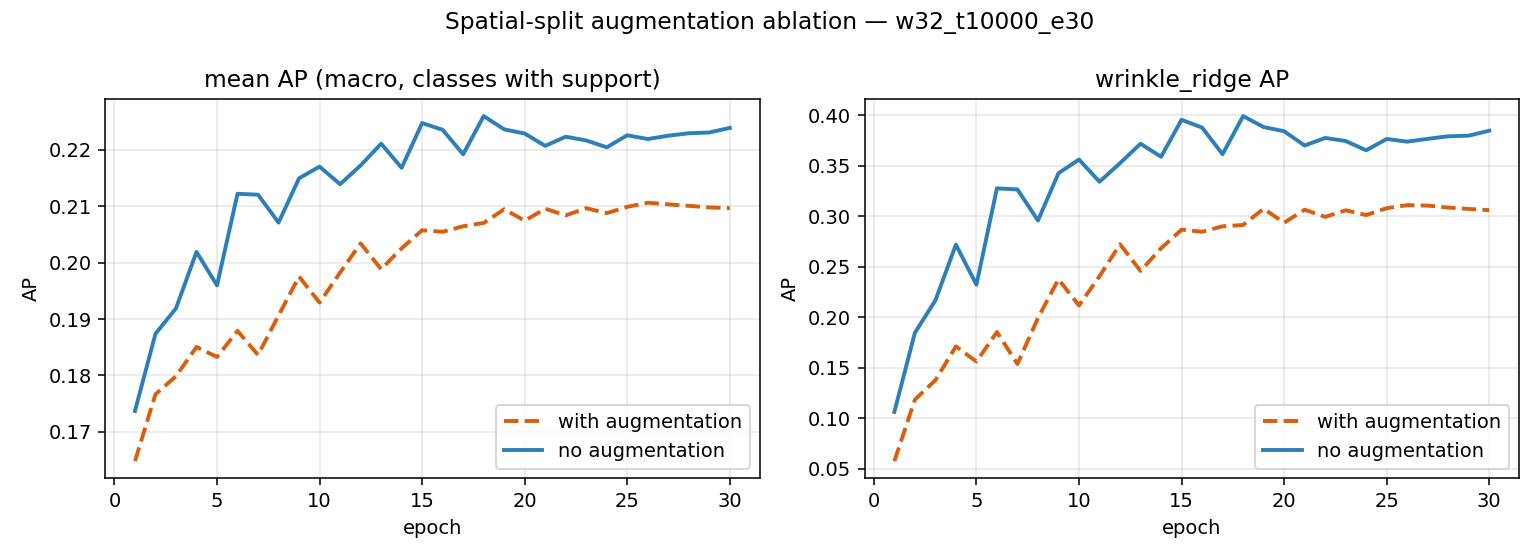
\includegraphics[width=0.85\columnwidth,keepaspectratio]{figures/MR/spatial_w32_t10000_e30_val_ap.png}
\caption{Validation AP across training epochs under the spatial split (macro mean over classes with support, left; \texttt{wrinkle\_ridge}, right). The no-augmentation arm dominates at every epoch on both metrics.}
\label{fig:spatial_rerun}
\end{figure}

The re-run \textbf{confirms the conclusion}: training without augmentation remains better, with the no-augmentation arm above the augmented one at every epoch (Fig.~\ref{fig:spatial_rerun}). The decomposition is, however, instructive. Absolute scores are substantially lower than on the leaky split (ridge AP 0.385 vs 0.558), confirming that random-split numbers were inflated by memorisation. The \emph{aggregate} advantage of no-augmentation also narrows (mean AP $+0.014$ here vs $+0.062$ on the leaky split), showing that part of the originally measured gap was indeed a split artefact. But for the direction-sensitive class the gap persists and is large --- ridge AP 0.385 vs 0.306, a 26\% relative difference on strictly disjoint validation pixels --- which is precisely the signature predicted by the geological explanation: augmentation hurts where orientation and illumination carry physical information. Confirmation at the full 15{,}931-tile T4 protocol remains scheduled, but the conclusion no longer rests on a confounded measurement.

\subsection{Qualitative Evaluation}
\label{sec:mr_qualitative}

Segmentation metrics alone do not reveal \emph{how} a model fails, so we complement the ablations with a visual comparison on identical validation tiles: raw image, ground truth, predicted probability, and a true-positive/false-positive/false-negative decomposition at threshold $0.5$, for the BCEDice baseline and the definitive model side by side.

\begin{figure}[htbp!]
\centering
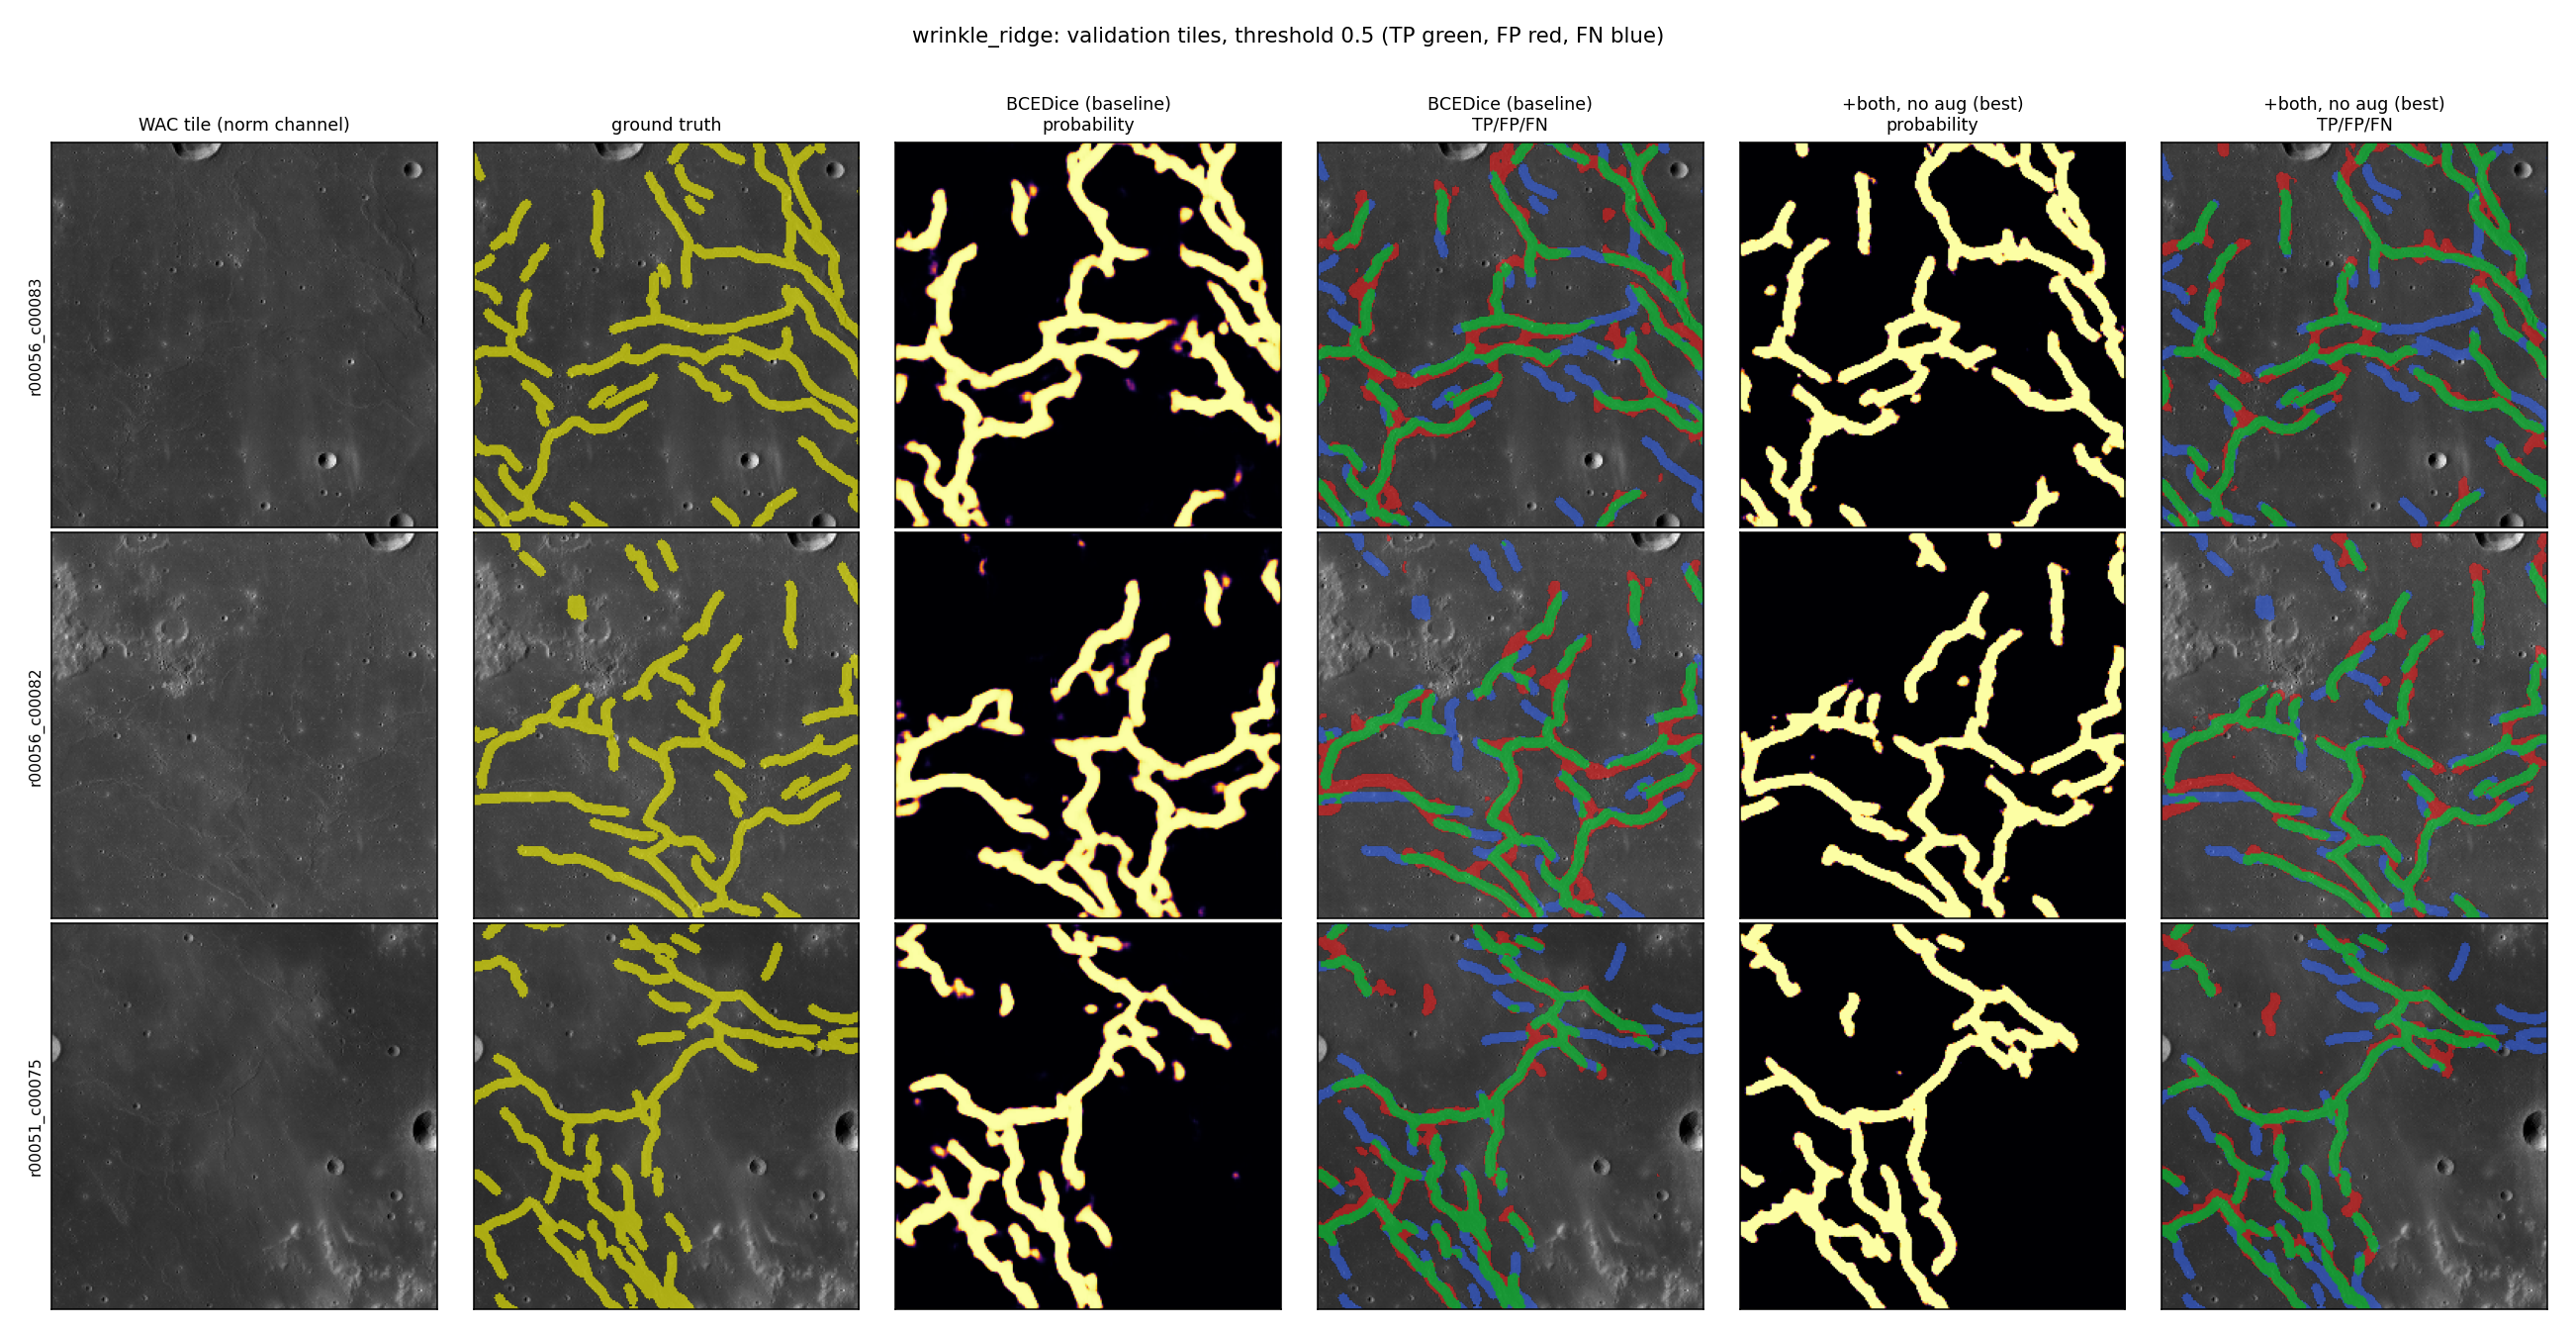
\includegraphics[width=0.85\columnwidth,keepaspectratio]{figures/MR/qualitative_wrinkle_ridge.png}
\caption{Wrinkle-ridge qualitative comparison on three validation tiles (TP green, FP red, FN blue). Both models recover the topology of the ridge network; the definitive model (+both, no augmentation) produces visibly more complete coverage and fewer false positives than the BCEDice baseline. Errors concentrate on thin, low-contrast ridge segments, consistent with the localisation difficulty of linear features.}
\label{fig:qualitative_ridge}
\end{figure}

\begin{figure}[htbp!]
\centering
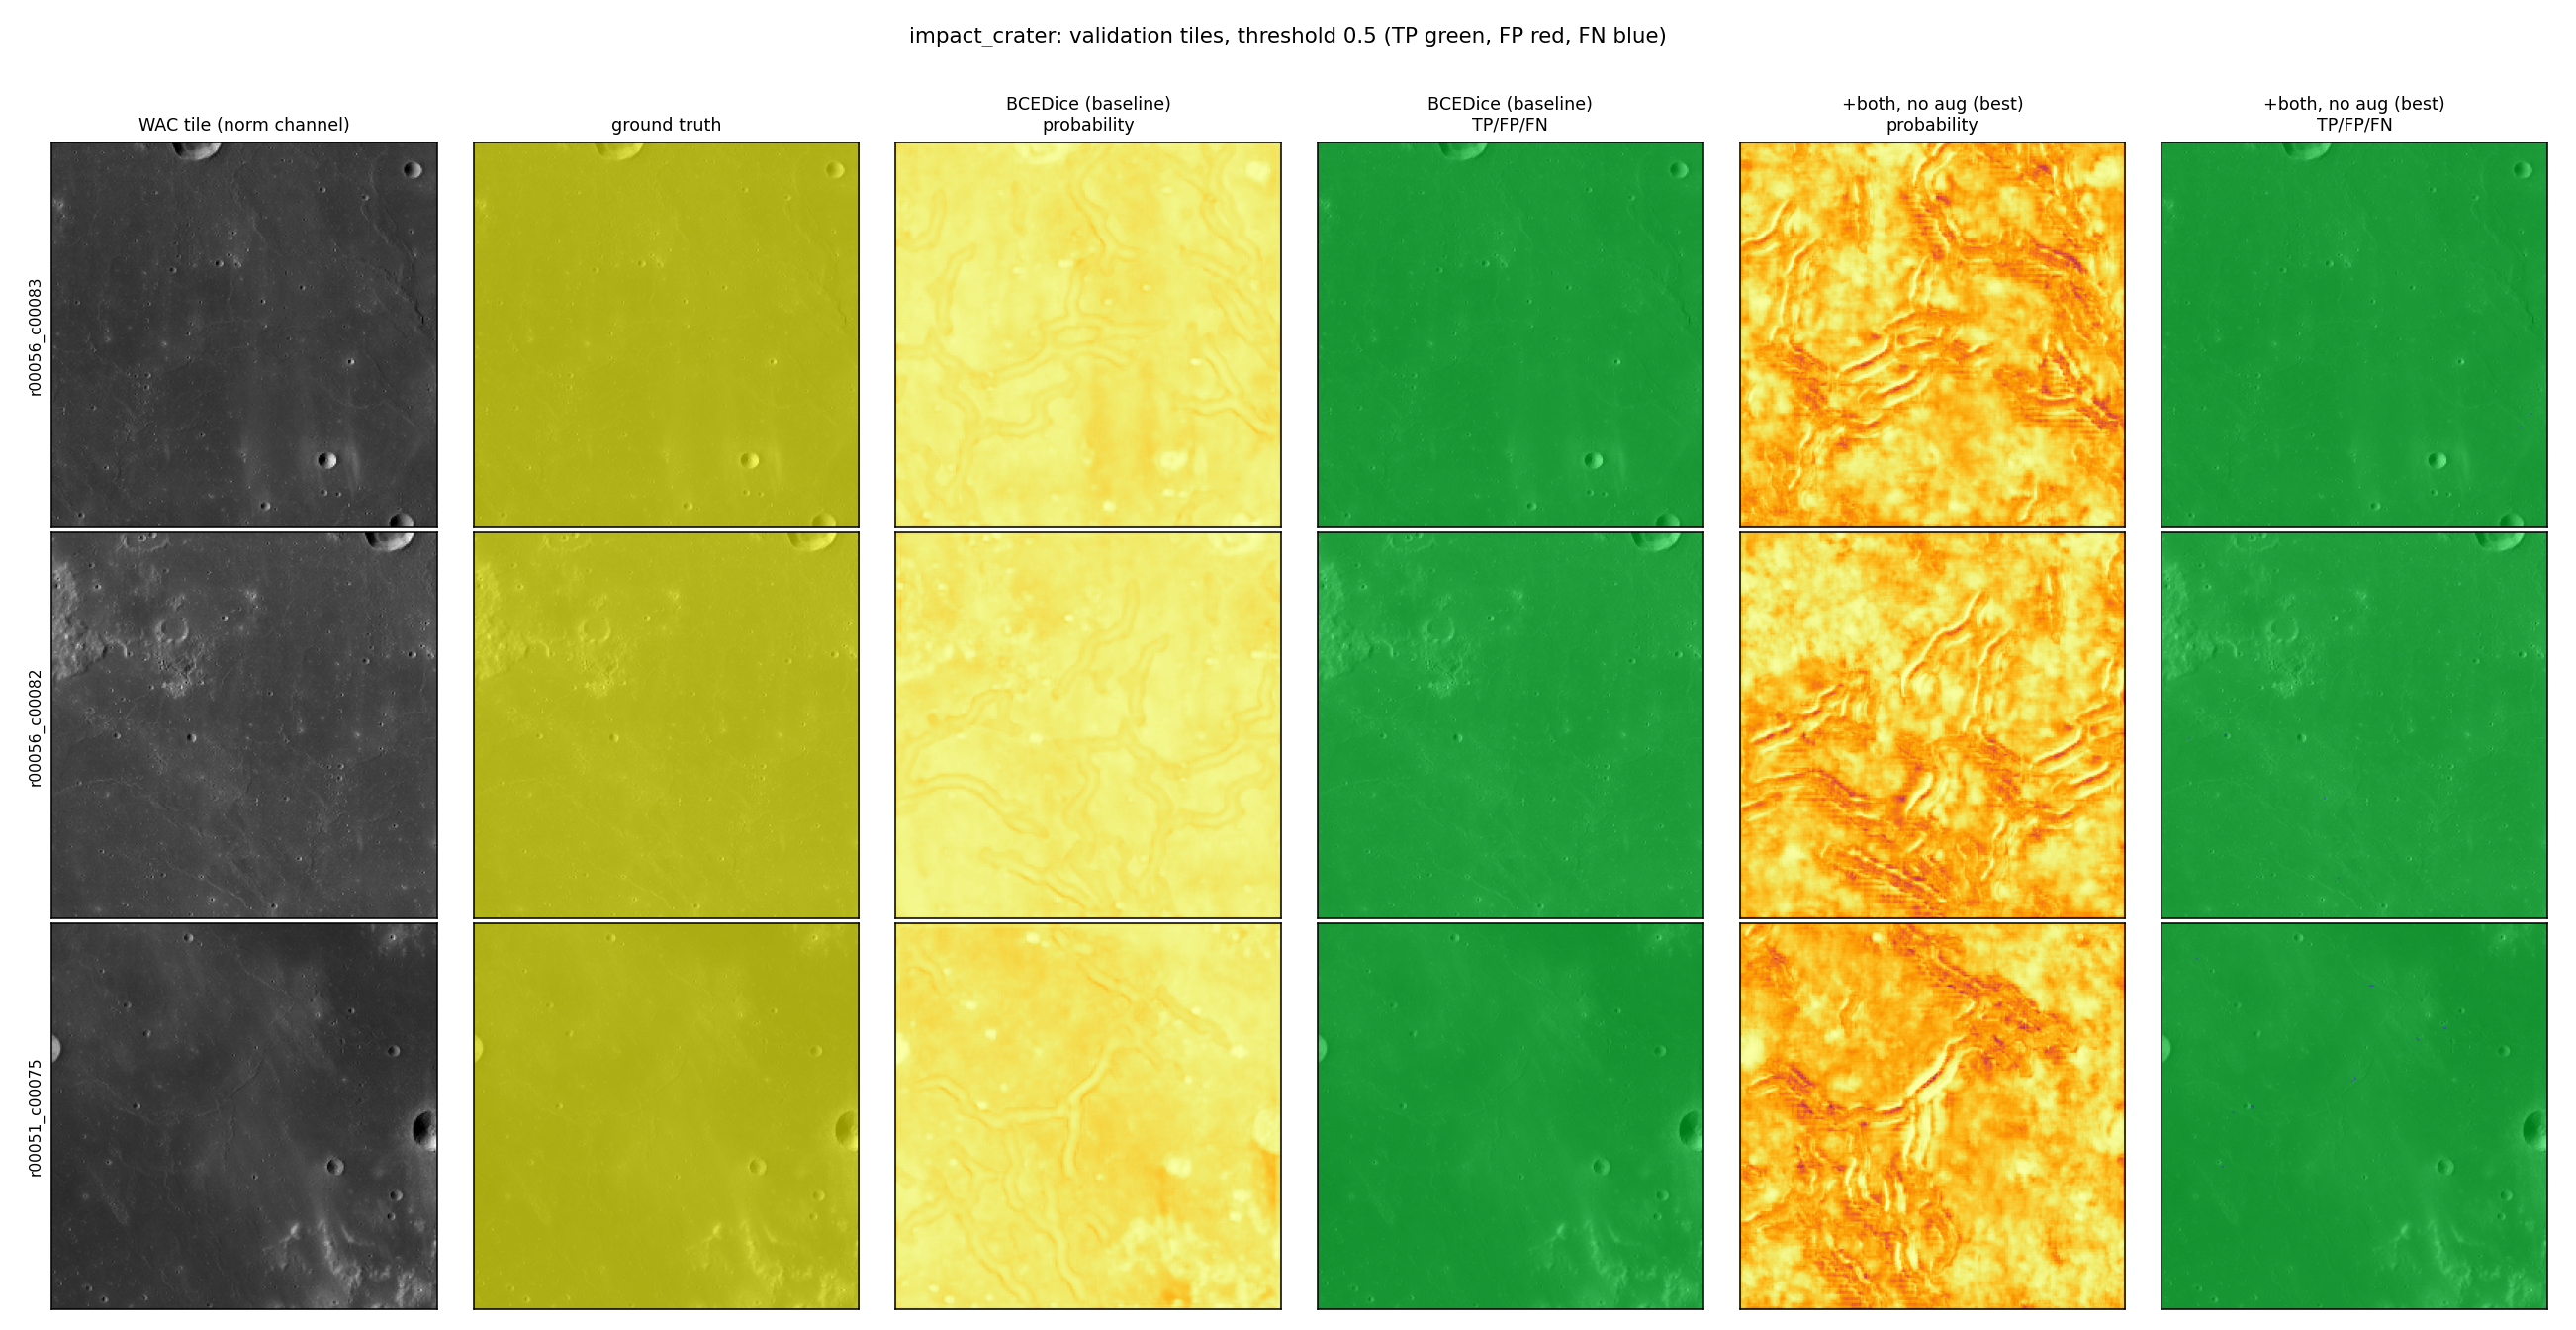
\includegraphics[width=0.85\columnwidth,keepaspectratio]{figures/MR/qualitative_impact_crater.png}
\caption{Impact-crater qualitative comparison on the same tiles. The ground truth covers the \emph{entire} tile (cf.\ the 82\% prevalence and 50.7\% fully-covered tiles of Table~\ref{tab:prevalence}), so a prediction of ``everywhere'' is trivially correct: this figure is direct visual evidence that the crater channel behaves as a near-coverage layer and that crater AP must be read against its 0.821 chance baseline.}
\label{fig:qualitative_crater}
\end{figure}

The ridge comparison shows that the metric gains of the definitive model correspond to a real, visible improvement in completeness of the recovered ridge network. The crater comparison, conversely, makes the saturation argument of Sec.~\ref{sec:mr_dataset} concrete.

\subsection{South Pole Inference}
\label{sec:mr_south_pole}

The best-performing model weights (\texttt{best\_trained.pth}) were applied to the lunar south pole to demonstrate transfer beyond the training region. The south pole imagery was obtained from the same LRO WAC source and tiled identically, producing 3{,}639 tiles. No feature catalogue exists for this region, so no ground-truth masks are available: the south-pole evaluation is necessarily based on prediction-confidence statistics (per-class maximum probabilities), not on accuracy metrics such as AP or IoU. The results below should therefore be read as transfer \emph{diagnostics} rather than as quantitative performance figures.

\paragraph{Inference pipeline.}
Each tile is preprocessed with the same CLAHE + Sobel three-channel pipeline. A sliding-window predictor runs the model tile by tile, saving per-class probability maps as compressed \texttt{.npz} files for downstream aggregation. Probability maps are aggregated over all tiles to compute global statistics.

\paragraph{Per-class results.}
Table~\ref{tab:south_pole_stats} reports the aggregated statistics over the 3{,}639 south pole tiles.

\begin{table}[htbp]
\centering
\caption{South pole inference results (3{,}639 tiles). Avg.\ Max.\ Prob.\ is the mean, over tiles, of the maximum predicted probability for each class. Global Max is the highest probability observed in any single tile.}
\label{tab:south_pole_stats}
\resizebox{\columnwidth}{!}{%
\begin{tabular}{lrrr}
\toprule
Class & Avg.\ Max.\ Prob. & Global Max & Status \\
\midrule
\texttt{impact\_crater}       & 0.863 & 1.000 & $\checkmark$ detected \\
\texttt{lobate\_scarp}        & 0.060 & 0.303 & weak \\
\texttt{pit\_skylight}        & 0.051 & 0.202 & weak \\
\texttt{irregular\_mare\_patch} & 0.040 & 0.215 & weak \\
\texttt{apollo\_site}         & 0.040 & 0.183 & weak \\
\texttt{candidate\_rille}     & 0.006 & 0.480 & sparse \\
\texttt{wrinkle\_ridge}       & 0.001 & 1.000 & sparse \\
\bottomrule
\end{tabular}
}
\end{table}

\begin{figure}[htbp!]
\centering
\begin{subfigure}[b]{0.48\textwidth}
    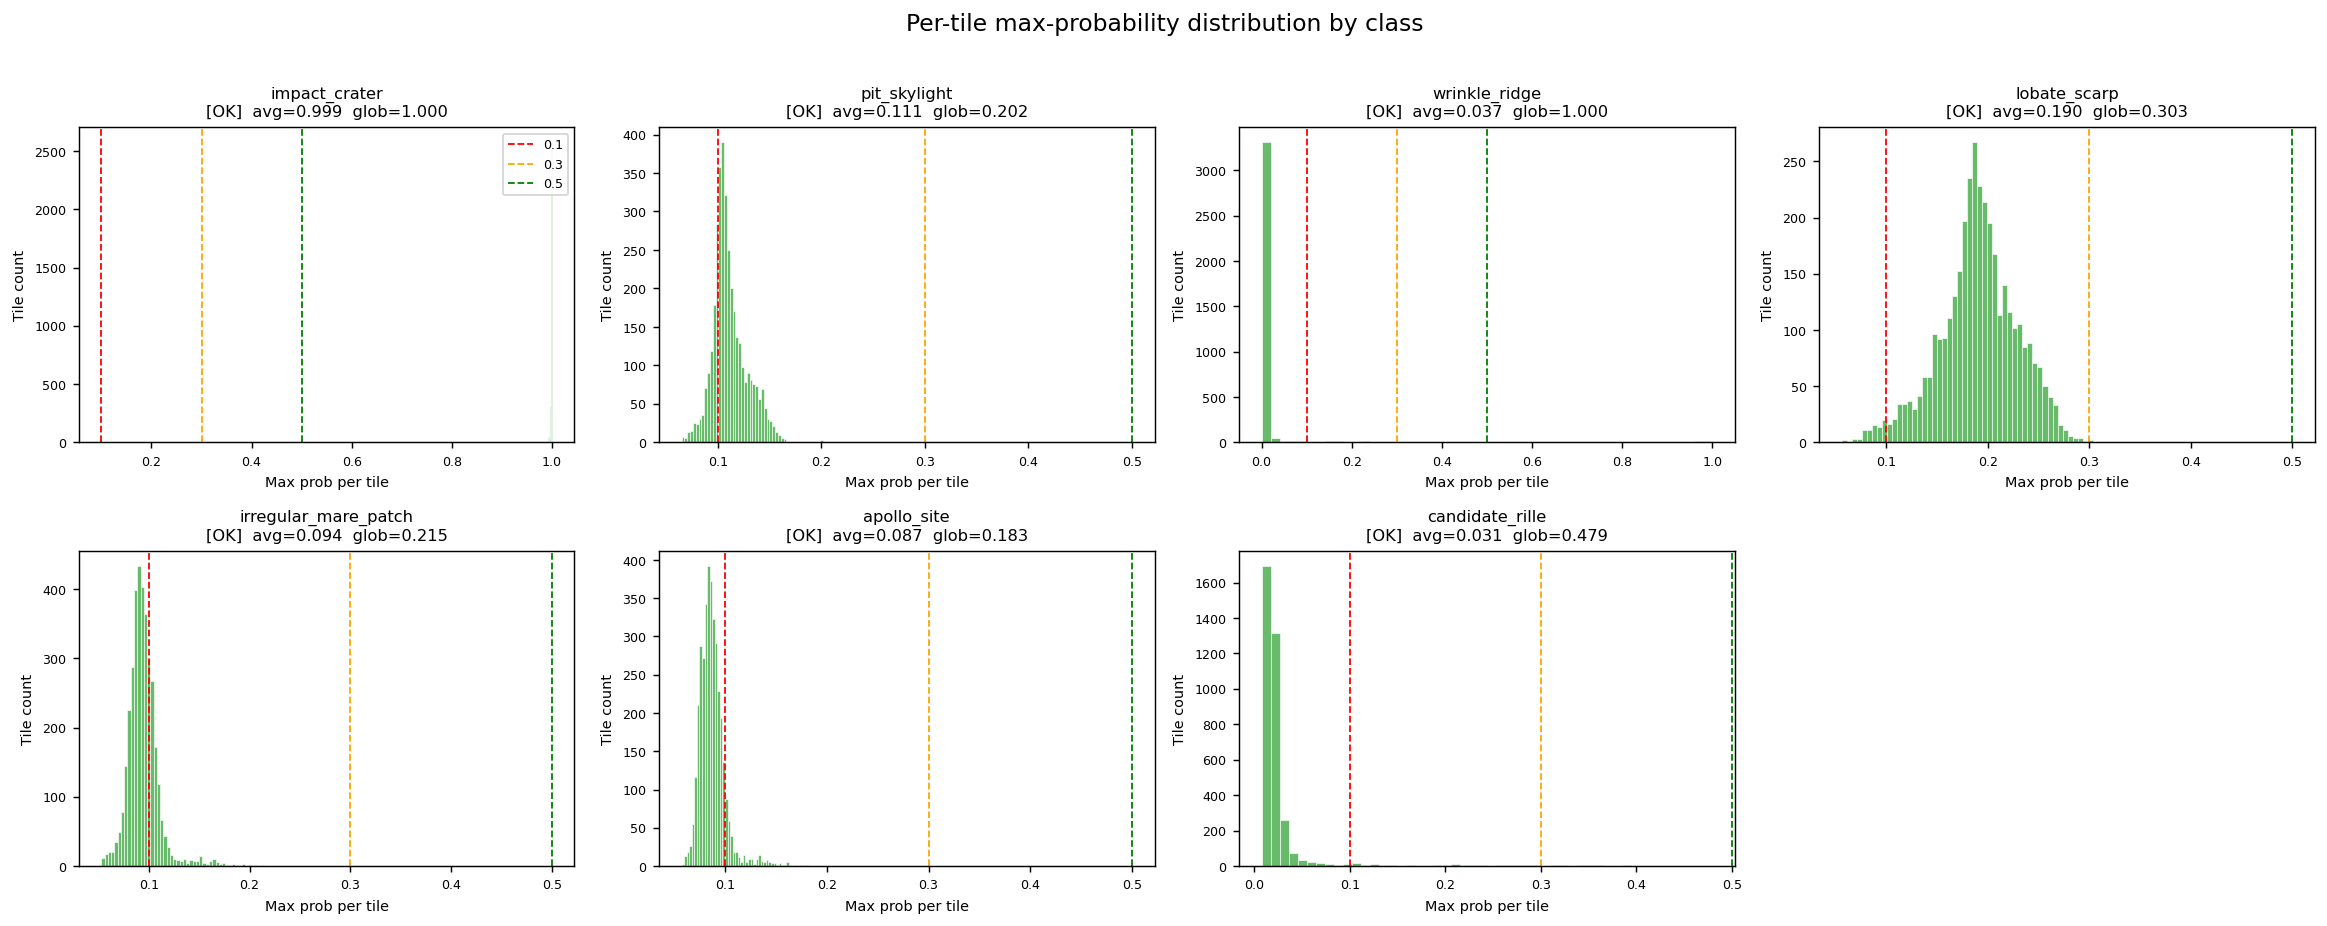
\includegraphics[width=\textwidth]{figures/MR/diagnostics_distributions.png}
    \caption{Per-tile max-probability distributions.}
\end{subfigure}
\hfill
\begin{subfigure}[b]{0.48\textwidth}
    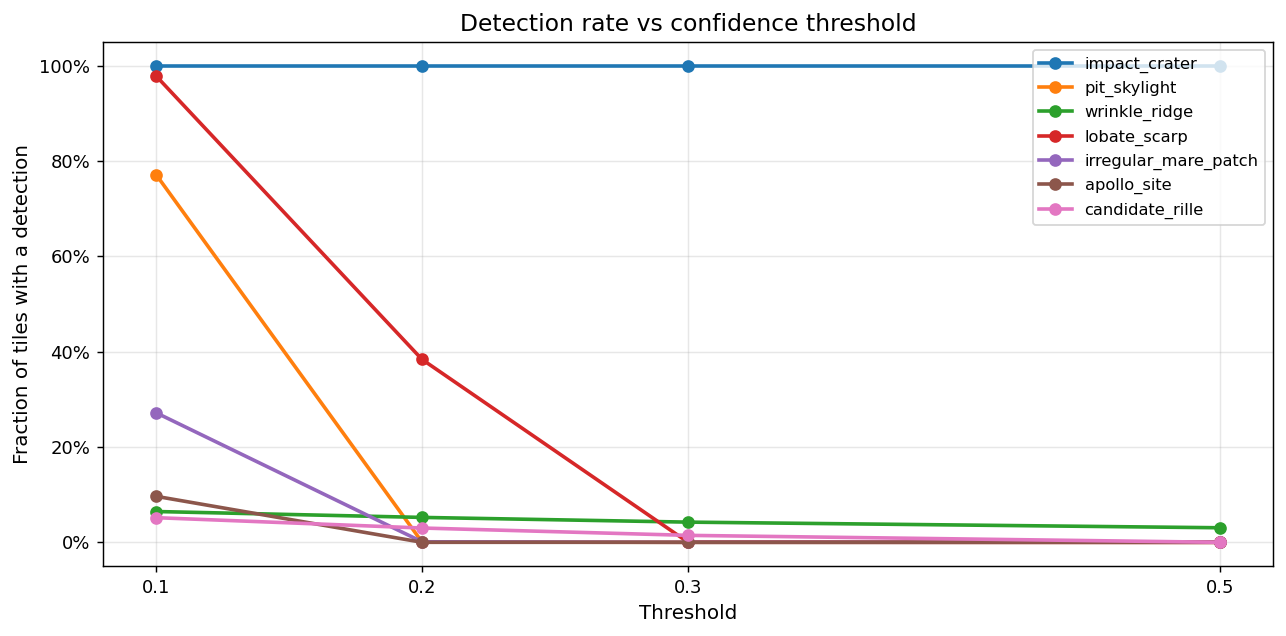
\includegraphics[width=\textwidth]{figures/MR/diagnostics_detection_rates.png}
    \caption{Detection rate vs.\ confidence threshold.}
\end{subfigure}
\caption{South pole inference diagnostics across 3{,}639 tiles. Impact craters are detected with near-certainty across the entire region. All other classes exhibit strongly right-skewed distributions with low average confidence, reflecting both the domain shift from Marius Hills and the scarcity of these features at the south pole.}
\label{fig:south_pole_diag}
\end{figure}

\begin{figure}[htbp!]
\centering
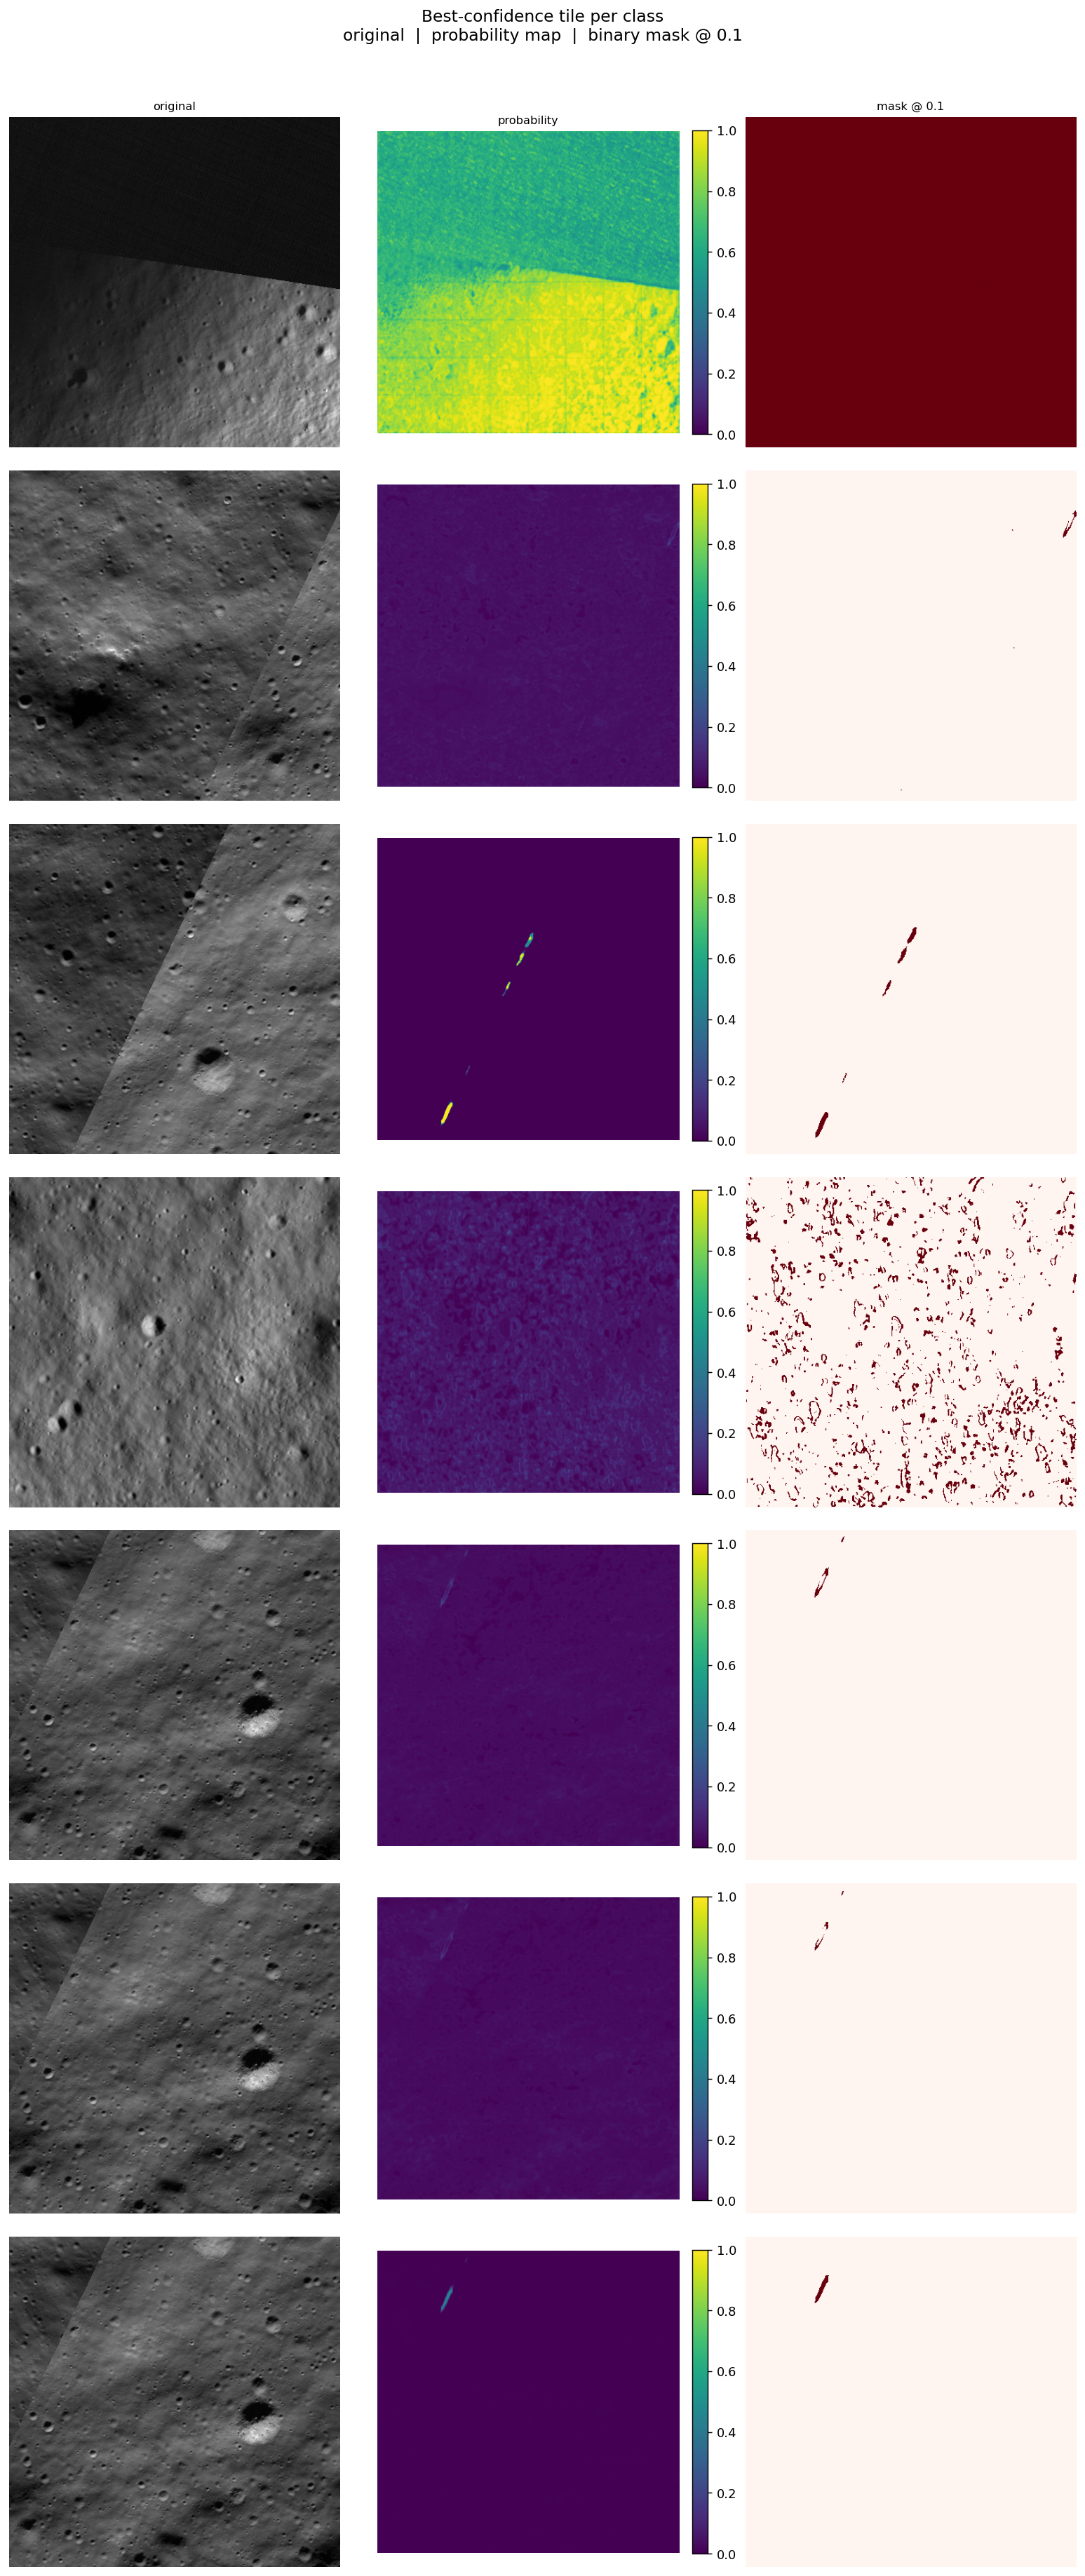
\includegraphics[width=0.85\columnwidth,keepaspectratio]{figures/MR/diagnostics_best_tiles.png}
\caption{Best-detected tile per class on the south pole imagery. Each panel shows the LRO WAC tile overlaid with the predicted probability map for the class with the highest maximum confidence in that tile. Note that overlays use a \emph{relative} threshold (top fraction of each tile's probabilities) so that the most likely candidate pixels are visible even when absolute confidence is low; coloured regions for the weak classes are therefore candidate locations, not confident detections. Impact craters stand out clearly; other classes show localised but low-confidence activations.}
\label{fig:south_pole_best}
\end{figure}

\paragraph{Analysis.}
The model assigns high crater probability across the entire south pole (average max probability 0.863). Given the near-saturated crater layer learned in training (Sec.~\ref{sec:mr_dataset}), this is expected behaviour --- the model has learned that almost everywhere is ``crater'' --- and should not be over-interpreted as precise crater delineation. Two classes --- \texttt{wrinkle\_ridge} and \texttt{candidate\_rille} --- show an interesting pattern: very low average-tile probabilities (0.001 and 0.006) but anomalously high global maxima (1.000 and 0.480). This indicates that the model makes rare but high-confidence predictions on a small number of tiles, rather than diffuse low-confidence activations everywhere.

The weak performance on rare classes at the south pole is attributable to two combined factors. First, the south pole is geologically distinct from Marius Hills: it lacks the volcanic structures (skylights, rilles, ridges) that dominate the training distribution, making it an out-of-distribution region for those classes. Second, the extremely low frequency of those classes in the training data means the model has seen very few positive examples even during Marius Hills training. Both issues motivate future work on label-efficient transfer learning and domain adaptation.

\subsection{Methodological Audit and Reproducibility}
\label{sec:mr_audit}

After the experimental campaign was completed, the entire pipeline --- code, data, report claims, and course guidance --- was subjected to a systematic audit. Every resulting change is a single, individually justified commit on the \texttt{U-net} branch, indexed in \texttt{Moon-Recognition/IMPROVEMENTS.md}; the executed notebooks were committed \emph{before} any fix, so the provenance of the published numbers is preserved. This section summarises what the audit found and how each finding affects the interpretation of the results --- both as a record for the group and because several findings changed the conclusions of this report.

\paragraph{(a) Report--code reconciliation.}
Several statements in an earlier draft did not match the implementation and were corrected against the code as ground truth: the CLAHE parameters (the pipeline uses \texttt{skimage} \texttt{equalize\_adapthist} with clip limit 0.03, not the OpenCV-style values previously quoted), the tiling description (tiles \emph{overlap} by 50\%), the split procedure (random permutation, not sequential), a gradient-clipping claim (clipping was never enabled), and a mis-attributed citation in the augmentation discussion (replaced with the correct survey~\cite{shorten2019augmentation}). The principle applied: any claim an examiner can check against the repository must be checkable.

\paragraph{(b) Train/validation leakage --- discovery and remedy.}
Because adjacent tiles share 50\% of their pixels, the random tile-level split leaks: a direct measurement on the real index showed that \textbf{100\% of the 3{,}186 validation tiles overlap at least one training tile}. This inflates absolute validation scores and specifically confounds the augmentation study, since a non-augmented model is freer to memorise tile appearance and a leaky validation set rewards exactly that memorisation. The remedy, recommended by the course material itself, is a \emph{spatial block split}: contiguous $1024$-px blocks are assigned to validation and every training tile whose footprint intersects a validation tile is discarded ($\texttt{data/splits.py}$; on the real index: 11{,}289 train / 3{,}248 validation tiles, 1{,}394 boundary tiles dropped, zero pixel overlap, verified by an independent assertion). The augmentation comparison was re-run under this split as a scaled paired protocol on local hardware (both arms share an identical split, initialisation, and schedule, so the comparison is internally valid); the conclusion was confirmed, with the expected partial decomposition into a leakage artefact and a genuine effect (Sec.~\ref{sec:mr_augmentation}). Full-protocol confirmation on CloudVeneto remains scheduled when GPU instances become available.

\paragraph{(c) Label audit --- channel saturation.}
A full pass over all 15{,}931 tiles produced the per-class prevalences of Table~\ref{tab:prevalence} and the central reinterpretation of this report: the \texttt{impact\_crater} channel covers 82.1\% of all pixels, making it a near-coverage layer whose AP must be read against a 0.821 chance baseline, while \texttt{wrinkle\_ridge} (prevalence $6.4\times10^{-3}$) emerges as the strongest genuine result and the five rarest classes turn out to have essentially no supervision at all. Without this audit, the headline claim of the report would have been the (nearly trivial) crater result.

\paragraph{(d) Qualitative evaluation.}
The course material requires visual evaluation alongside metrics. Figures~\ref{fig:qualitative_ridge} and~\ref{fig:qualitative_crater} (generated by \texttt{scripts/qualitative\_eval.py} from the full-run checkpoints) confirm both audit findings visually: the metric advantage of the definitive model corresponds to a visibly more complete ridge reconstruction, and the crater ground truth fills entire tiles.

\paragraph{(e) Engineering fixes.}
The audit also produced functional fixes, each preserving the published numbers: evaluation memory reduced by ${\sim}12$\,GB with results verified bit-identical; undefined metrics for classes absent from a validation split now reported as NaN with an explicit support count rather than as a spurious 0; checkpoint loading made compatible with PyTorch $\geq 2.6$ and made loud on architecture/checkpoint mismatches (previously a mismatch silently produced random predictions); the sliding-window inference default aligned with the 256-px training context; dead machine-specific paths removed from the data manifest; and the training configuration file synchronised with the protocol actually used for the published runs.

\subsection{Summary and Conclusions}
\label{sec:mr_conclusions}

Table~\ref{tab:final_summary} collects the final T4 results for the best configuration identified in each study. The definitive model for the project is \textbf{SmallUNet with $w=32$, FocalDice loss, residual shortcuts, bottleneck dropout ($p=0.3$), trained without augmentation for 30 epochs on the full 15{,}931-tile Marius Hills dataset}. Its weights are stored as \texttt{data/MR/weights/best\_trained.pth}.

One caveat applies to this synthesis across studies. The architecture ablation (Study~1) and the width sweep (Study~2) were run \emph{with} augmentation enabled, before Study~3 established that augmentation is harmful on this dataset; their rankings are therefore strictly established \emph{under augmentation}. The components they select --- residual shortcuts and a moderate width ($w=32$) --- are architectural choices not expected to interact strongly with geometric augmentation, so we adopt them for the definitive (no-augmentation) model; re-confirming the architecture and width rankings directly in the no-augmentation regime nonetheless remains the natural next experiment.

\begin{table}[htbp]
\centering
\caption{Best result from each ablation study (full T4 run, 30 epochs).}
\label{tab:final_summary}
\resizebox{\columnwidth}{!}{%
\begin{tabular}{llrrrr}
\toprule
Study & Best config & Params & Mean F1 & Mean AP & Ridge AP \\
\midrule
Architecture & +both ($w=32$, augmented) & 2.0M & 0.2076 & 0.2004 & 0.453 \\
Width        & wide ($w=64$, augmented)  & 8.0M & 0.2153 & 0.2016 & 0.445 \\
Augmentation & +both, $w=32$, \textbf{no aug} & 2.0M & \textbf{0.2986} & \textbf{0.2647} & \textbf{0.558} \\
\bottomrule
\end{tabular}
}
\end{table}

The principal conclusions of this study are:

\begin{enumerate}
    \item \textbf{Residual shortcuts help; dropout alone does not.} Adding residual connections to DoubleConv blocks consistently improves all aggregate metrics. Bottleneck dropout in isolation hurts performance, likely because sparse labels already regularise the network. The combination \textbf{+both} yields the best augmented-training result.

    \item \textbf{Network width exhibits strong diminishing returns.} The small model ($w=16$, 505K parameters) achieves a mean AP within 0.001 of the wide model ($w=64$, 8M parameters) at one-sixth the training time and ${\sim}16\times$ fewer parameters. For resource-constrained inference the small model is recommended.

    \item \textbf{Geometric augmentation is harmful on this dataset --- confirmed under a leakage-free split.} Training without flips and rotations outperforms the augmented model on the original random split, and the advantage survives the spatial block split re-run with strictly disjoint validation pixels (ridge AP 0.385 vs 0.306, no-augmentation above at every epoch). The decomposition is informative: part of the aggregate gap on the random split was a leakage artefact, but the direction-sensitive classes retain a large genuine gap, exactly as predicted by the directional bias of the Marius Hills linear features and the fixed illumination geometry. Augmentation strategies must be tailored to the structural properties of the target domain.

    \item \textbf{Crater AP must be read against its prevalence baseline; ridges are the strongest genuine result.} The \texttt{impact\_crater} channel covers 82.1\% of all pixels (half of the tiles are fully positive), so its AP $\approx 0.95$ is only a modest lift over the 0.821 chance level --- the channel behaves as a near-coverage layer, and Fig.~\ref{fig:qualitative_crater} shows that predicting ``everywhere'' is trivially correct. By contrast, \texttt{wrinkle\_ridge} has a prevalence of $6.4\times10^{-3}$, so the best ridge AP of 0.558 is ${\sim}90\times$ chance level and corresponds to a visibly accurate reconstruction of the ridge network (Fig.~\ref{fig:qualitative_ridge}). The remaining five classes have prevalences below $1.4\times10^{-4}$ --- their near-zero scores reflect the absence of supervision, not a failure of the architecture. The seven-class macro AP of 0.265 is therefore a conservative aggregate, depressed by these five unsupervised channels; the model's genuine performance is read more faithfully per class against chance (crater $\approx0.95$ vs the 0.821 baseline, ridge 0.558 vs 0.0064) than from the macro mean alone.

    \item \textbf{South pole transfer is limited by domain shift and label scarcity.} The model accurately maps impact craters but provides only weak signals for rarer geomorphological features. Acquiring labels for even a small number of south-pole-specific tiles, or employing few-shot domain adaptation, is likely necessary for reliable multi-class south-pole mapping.
\end{enumerate}

\section{YOLO-Based Detection of Lunar Surface Features}

\subsection{YOLO-Based Object Detection} 
Prior work on object detection repurposes classifiers to perform detection. In contrast, modern approaches frame object detection as a regression problem, simultaneously predicting spatially separated bounding boxes and their associated class probabilities. In this formulation, a convolutional neural network (CNN) processes an entire image in a single forward pass, directly outputting bounding box coordinates and class probabilities without intermediate steps.
\subsection{Two-Stage vs. Single-Stage Detection}
\subsubsection{Two-Stage Detection: R-CNN and Variants}
R-CNN and its variants operate through two sequential stages. In the first stage — addressing "Where?" — a Region Proposal Network (RPN) scans the entire image and generates hundreds of candidate bounding boxes, known as Regions of Interest (RoIs), identifying locations where an object might exist. In the second stage — addressing "What?" — each proposed region is individually passed through a CNN to classify the object it contains and refine the box coordinates. While thorough, this two-stage pipeline is computationally expensive and ill-suited for real-time applications.
\subsubsection{Single-Stage Detection: YOLO}
You Only Look Once (YOLO) eliminates the region proposal stage entirely. The input image is divided into a grid, and each grid cell simultaneously predicts both the bounding box coordinates and the class probabilities of any object it contains. All predictions are generated in a single forward pass through the network — the image enters, and detections are produced immediately. This architecture makes YOLO significantly faster than R-CNN-based methods while maintaining competitive accuracy, making it well-suited for real-time detection tasks.
\subsection{Applications of YOLO in Scientific Domains}
The YOLO architecture has been widely adopted across diverse scientific and engineering domains. Notable applications include photovoltaic (PV) fault detection via thermal imaging (Prajapati et al.), hotspot detection using YOLOv3 combined with infrared thermography (Tajwar et al.), aerial UAV-based PV panel inspection (Greco et al.), cloud-edge defect detection using YOLOv3-tiny (Wang et al.), 5G drone-assisted inspection with YOLOv4 (Zou et al.), electroluminescence image analysis with YOLO-PV (Meng et al.), multi-defect detection using GBH-YOLOv5 (Li et al.), image fusion with YOLOv5 and ResNet (Hong et al.), UAV hotspot detection with S-YOLOv5 (Zheng et al.), UAV thermal imaging using YOLOv5 (Zhang et al.), parameter optimization with YOLOv8 and Particle Swarm Optimization (Phan et al.), and a hybrid Transformer-YOLO architecture known as PV-YOLO (Yin et al.).
\subsection{YOLOv8:Advancements}
Ultralytics, the primary maintainer of modern YOLO releases, redefined the framework with the introduction of YOLOv8 in 2023. YOLOv8 incorporates a decoupled detection head, anchor-free predictions, and refined training strategies, resulting in substantial improvements in both accuracy and deployment versatility. It achieved broad industrial adoption owing to its clean Python API, compatibility with TensorRT, CoreML, and ONNX export formats, and the availability of model variants spanning a range of speed-accuracy trade-offs: nano, small, medium, large, and extra-large.
YOLOv8 builds upon the foundations established by its predecessors in the YOLO family, integrating advances in neural network design and training methodology. Like earlier versions, it unifies object localization and classification within a single, end-to-end differentiable network, preserving the balance between inference speed and detection accuracy. 
\subsection{Dataset}

The dataset used in this study comprises annotations for seven distinct lunar surface 
feature classes: impact crater, pit skylight, wrinkle ridge, lobate scarp, irregular 
mare patch, Apollo site, and candidate rille. As illustrated in Figure~\ref{fig:class_dist}, 
the class distribution is highly imbalanced. The dominant class, \textit{impact crater}, 
accounts for 382,122 instances — representing approximately 95.51\% of the total annotation 
count — owing to the widespread and frequent occurrence of impact craters across the lunar 
surface. The remaining six classes are considerably underrepresented: wrinkle ridge 
contributes 16,133 instances ($\sim$4.03\%), followed by lobate scarp (674), pit skylight 
(328), irregular mare patch (191), Apollo site (161), and candidate rille (82), the last 
three collectively accounting for less than 0.1\% of the dataset.

This severe class imbalance poses a significant challenge for model training, as the 
detector may develop a strong bias toward predicting the dominant impact crater class 
while failing to generalize to the rare feature types. Furthermore, all annotated objects 
exhibit very small bounding box dimensions relative to the image size, with the majority 
of boxes spanning approximately 5\% of the image width and height. These characteristics 
— extreme class imbalance and small object scale — collectively present challenges that 
must be addressed during model development to achieve reliable multi-class detection.

Table~\ref{tab:class_dist} summarizes the per-class instance counts and their 
proportional contributions to the full dataset.

%------------------------------------------------------------------
%  TABLE
%------------------------------------------------------------------
\begin{table}[htbp]
\centering
\caption{Per-class instance distribution in the lunar surface feature dataset.}
\label{tab:class_dist}
\resizebox{\columnwidth}{!}{%
\begin{tabular}{llrr}
\hline
\textbf{Class ID} & \textbf{Class Label} & \textbf{Instances} & \textbf{Proportion (\%)} \\
\hline
class0 & Impact Crater         & 382,122 & 95.51 \\
class2 & Wrinkle Ridge         &  16,133 &  4.03 \\
class3 & Lobate Scarp          &     674 &  0.17 \\
class1 & Pit Skylight          &     328 &  0.08 \\
class4 & Irregular Mare Patch  &     191 &  0.05 \\
class5 & Apollo Site           &     161 &  0.04 \\
class6 & Candidate Rille       &      82 &  0.02 \\
\hline
\textbf{Total} & & \textbf{399,691} & \textbf{100.00} \\
\hline
\end{tabular}
}
\end{table}

%------------------------------------------------------------------
%  FIGURE
%------------------------------------------------------------------
\begin{figure}[htbp!]
    \centering
    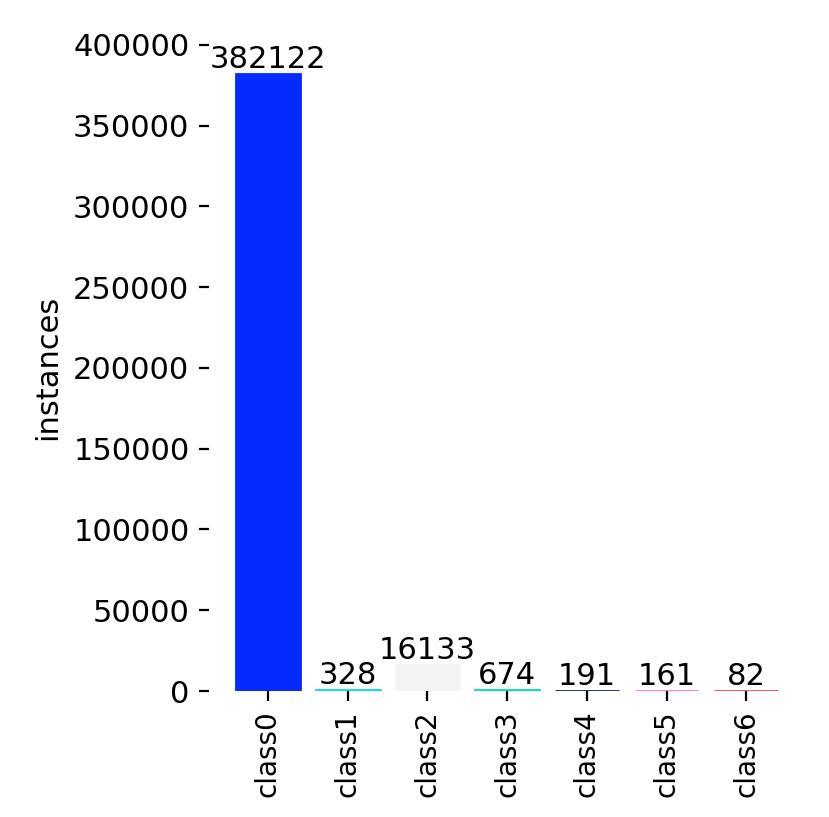
\includegraphics[width=0.85\linewidth]{./imageswithzero/labels_copy.jpg}
    \caption{Class instance distribution of the lunar surface feature dataset across 
    seven categories. The impact crater class (class0) dominates with 382,122 instances, 
    representing 95.51\% of all annotations, highlighting a severe class imbalance 
    relative to the remaining six feature types.}
    \label{fig:class_dist}
\end{figure}


%------------------------------------------------------------------
%  FIGURE
%------------------------------------------------------------------
\begin{figure}[htbp!]
    \centering
    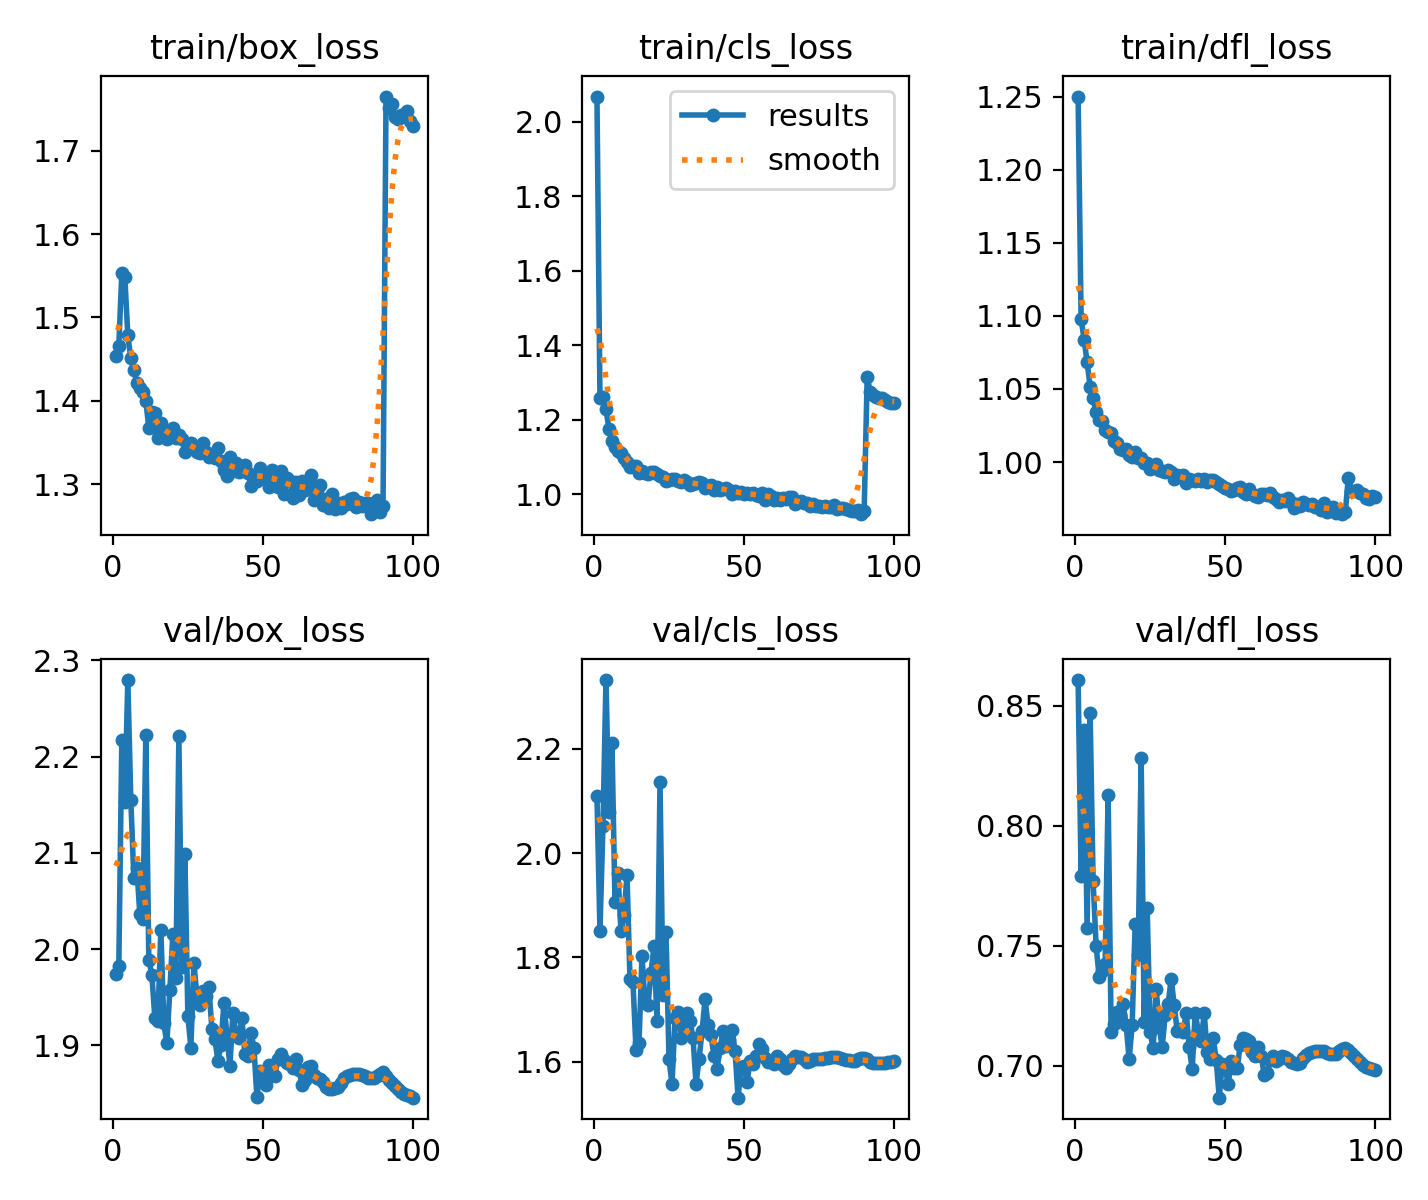
\includegraphics[width=0.95\linewidth]{./imageswithzero/loss.png}
    \caption{Training and validation loss curves over 100 epochs for the YOLOv8n 
    lunar feature detection model, including bounding box loss (box\_loss), 
    classification loss (cls\_loss), and distribution focal loss (dfl\_loss).}
    \label{fig:loss_curves}
\end{figure}
%------------------------------------------------------------------
%  FIGURE
%------------------------------------------------------------------

%------------------------------------------------------------------
%  FIGURE


%------------------------------------------------------------------
%  FIGURE
%------------------------------------------------------------------



%------------------------------------------------------------------
%  TEXT
%------------------------------------------------------------------
\subsubsection{Training and Validation Loss}

Figure~\ref{fig:loss_curves} presents the evolution of the three loss components 
— box loss, classification loss, and distribution focal loss (DFL) — across 100 
training epochs, evaluated on both the training and validation sets.

All three training losses exhibit a consistent downward trend, indicating stable 
and progressive model convergence. A transient spike is observed near epoch 90 
across all training losses, attributable to the cosine annealing learning rate 
scheduler employed by YOLOv8, which periodically resets the learning rate to 
escape local minima. The final training losses reached approximately 1.28 
(box), 0.97 (cls), and 0.97 (dfl).

The validation losses follow a similar decreasing trajectory, stabilizing at 
approximately 1.85 (box\_loss), 1.60 (cls\_loss), and 0.70 (dfl\_loss) by the 
final epoch. The persistent gap between training and validation losses suggests mild 
overfitting, likely exacerbated by the dominance of the impact crater class and 
the limited number of instances for the remaining six categories.

%------------------------------------------------------------------
%  TABLE
%------------------------------------------------------------------
%------------------------------------------------------------------
%  TABLE
%------------------------------------------------------------------
\begin{table}[htbp]
\centering
\caption{Per-class instance distribution of the reduced dataset after excluding 
the impact crater class.}
\label{tab:class_dist_reduced}
\resizebox{\columnwidth}{!}{%
\begin{tabular}{llrr}
\hline
\textbf{Class ID} & \textbf{Class Label} & \textbf{Instances} & \textbf{Proportion (\%)} \\
\hline
class1 & Wrinkle Ridge        & 16,115 & 92.59 \\
class2 & Lobate Scarp         &    664 &  3.81 \\
class0 & Pit Skylight         &    311 &  1.79 \\
class4 & Apollo Site          &    156 &  0.90 \\
class3 & Irregular Mare Patch &    148 &  0.85 \\
class5 & Candidate Rille      &     92 &  0.53 \\
\hline
\textbf{Total} & & \textbf{17,486} & \textbf{100.00} \\
\hline
\end{tabular}
}
\end{table}

%------------------------------------------------------------------
%  TEXT
%------------------------------------------------------------------
% Table~\ref{tab:class_dist_reduced} summarizes the class distribution of the 
% reduced dataset after the removal of the impact crater class. The total number 
% of annotations decreased substantially from 399,691 to 17,486 instances. 
% While the exclusion of the dominant class significantly reduces the overall 
% imbalance magnitude, the wrinkle ridge class (class1) remains the most 
% prevalent category with 16,115 instances, representing 92.59\% of the reduced 
% dataset. The remaining five classes are considerably underrepresented: lobate 
% scarp accounts for 664 instances (3.81\%), followed by pit skylight (311, 
% 1.79\%), Apollo site (156, 0.90\%), irregular mare patch (148, 0.85\%), and 
% candidate rille (92, 0.53\%). These proportions indicate that class imbalance 
% persists in the reduced dataset, albeit in a less extreme form than in the 
% original. This residual imbalance should be taken into consideration when 
% interpreting detection performance across individual classes, particularly 
% for the three least-represented categories which together account for under 
% 2\% of all annotations.

%------------------------
%------------------------------------------------------------------
%  SUBSECTION
%------------------------------------------------------------------
\subsubsection{Detection Without Impact Craters}

To address the severe class imbalance identified, 
a second experiment was conducted in which the dominant impact crater class was excluded from the dataset (Table~\ref{tab:class_dist_reduced}). The remaining six classes were retained: 
pit skylight, wrinkle ridge, lobate scarp, irregular mare patch, Apollo site, 
and candidate rille.

%------------------------------------------------------------------
%  FIGURE 1 — labels
%------------------------------------------------------------------
\begin{figure}[htbp!]
    \centering
    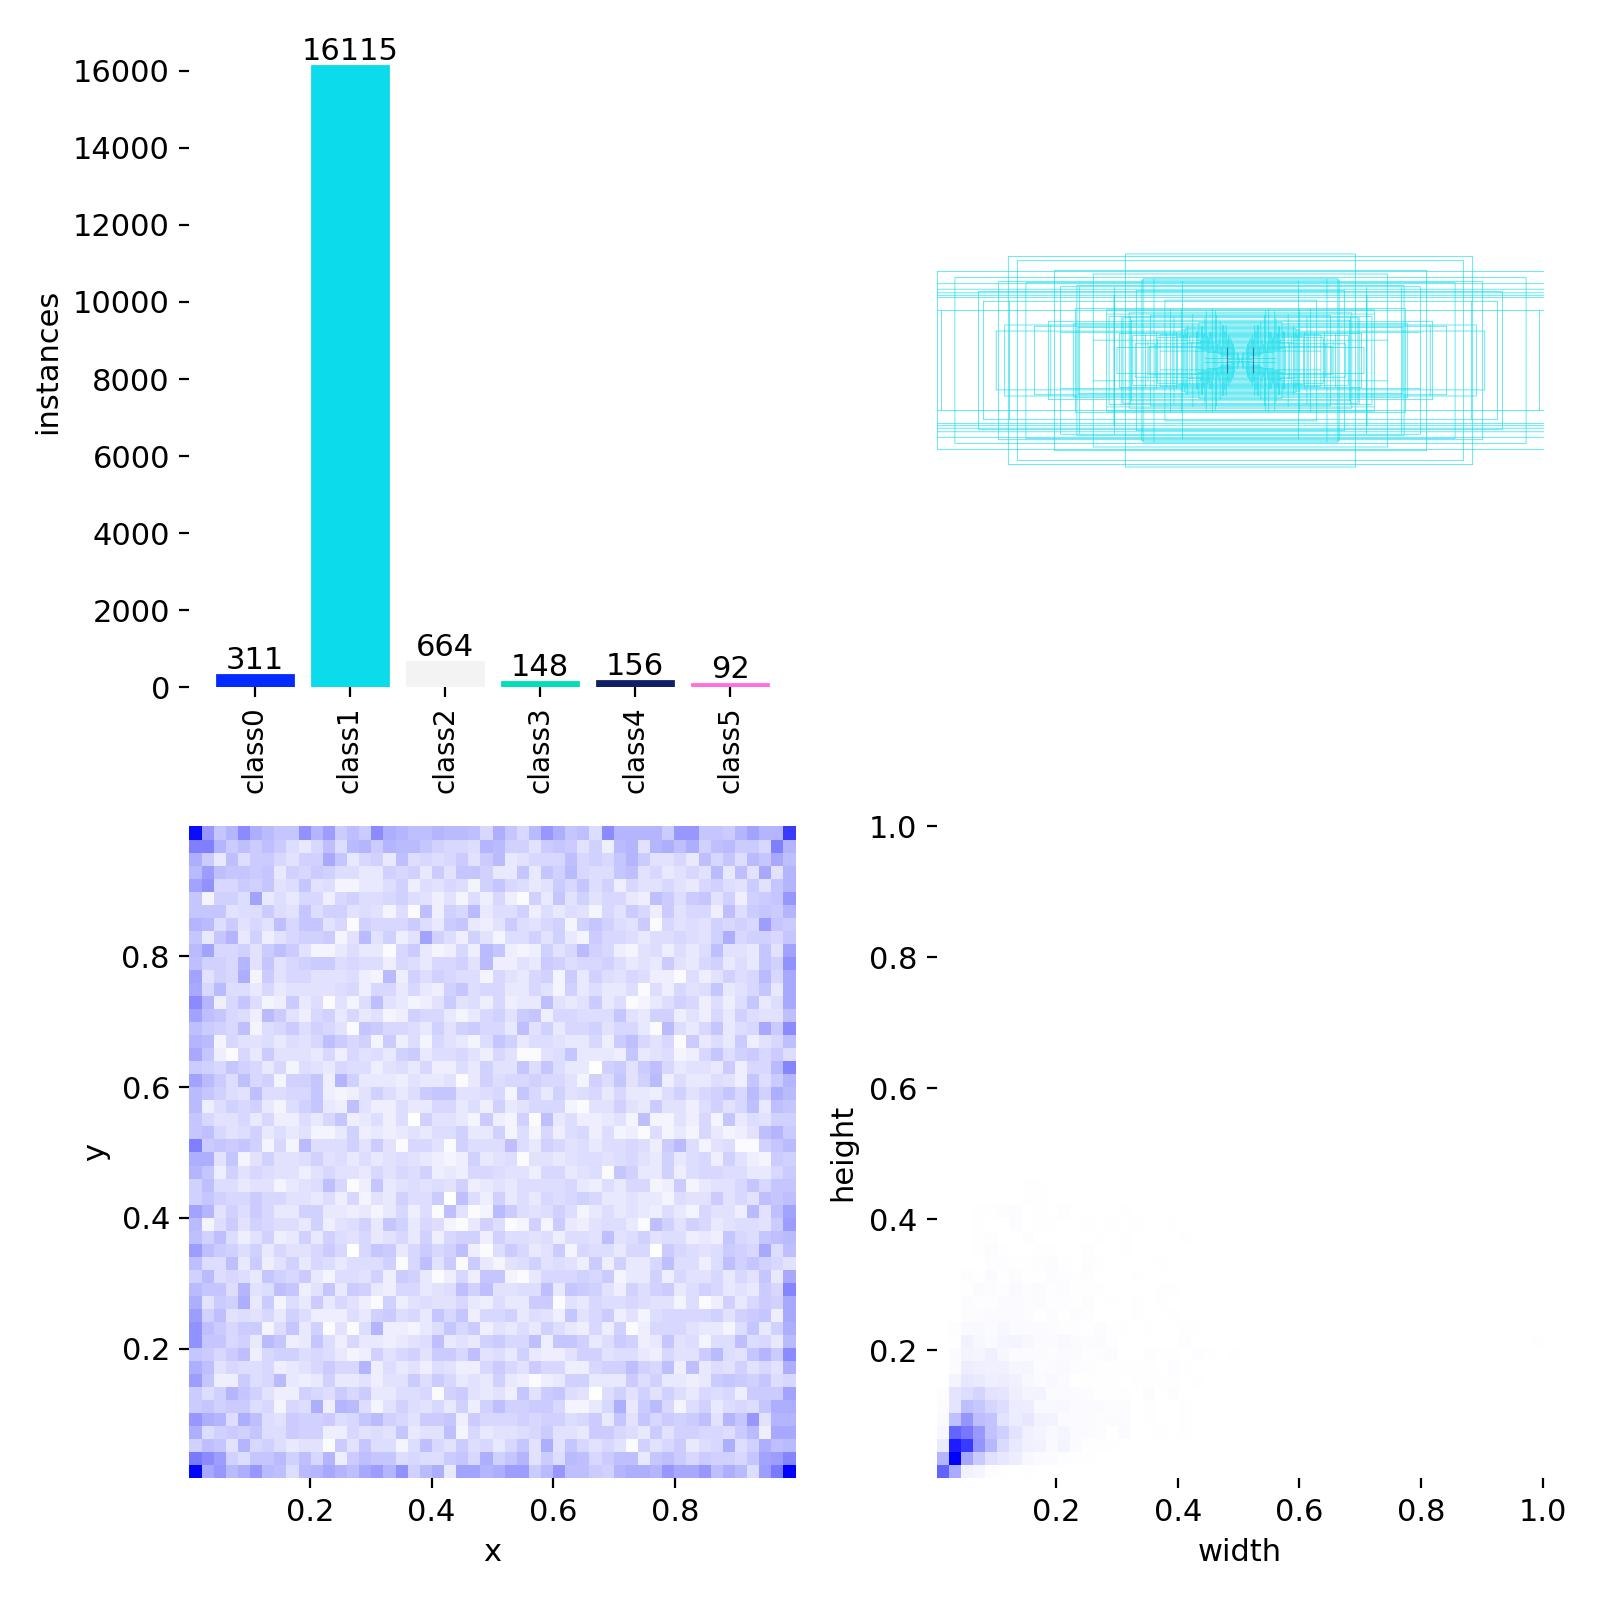
\includegraphics[width=0.85\linewidth]{imageswithoutzero/labels(1).jpg}
    \caption{Class instance distribution and spatial statistics of the reduced 
    dataset after removing the impact crater class. The wrinkle ridge class (class1) 
    now dominates with 16,115 instances, followed by lobate scarp (664), Apollo site 
    (156), pit skylight (148), impact crater (311), and candidate rille (92). 
    The spatial heatmap shows a more uniform distribution of object centers across 
    the image plane, while bounding boxes remain concentrated at small 
    width-height values ($<$0.2), confirming the small-scale nature of the 
    detected features.}
    \label{fig:labels_reduced}
\end{figure}

Figure~\ref{fig:labels_reduced} shows the label statistics of the reduced dataset. 
Compared to the full dataset, the class distribution is considerably less extreme, 
with wrinkle ridge (class1) becoming the dominant class at 16,115 instances. 
Notably, the spatial heatmap of object center coordinates (x, y) now exhibits a 
near-uniform spread across the image plane, in contrast to the left-center 
concentration observed previously. The width-height distribution remains tightly 
clustered near zero, confirming that all target features are small relative to 
the image dimensions.

%------------------------------------------------------------------
%  FIGURE 2 — training batch
%------------------------------------------------------------------
\begin{figure}[htbp!]
    \centering
    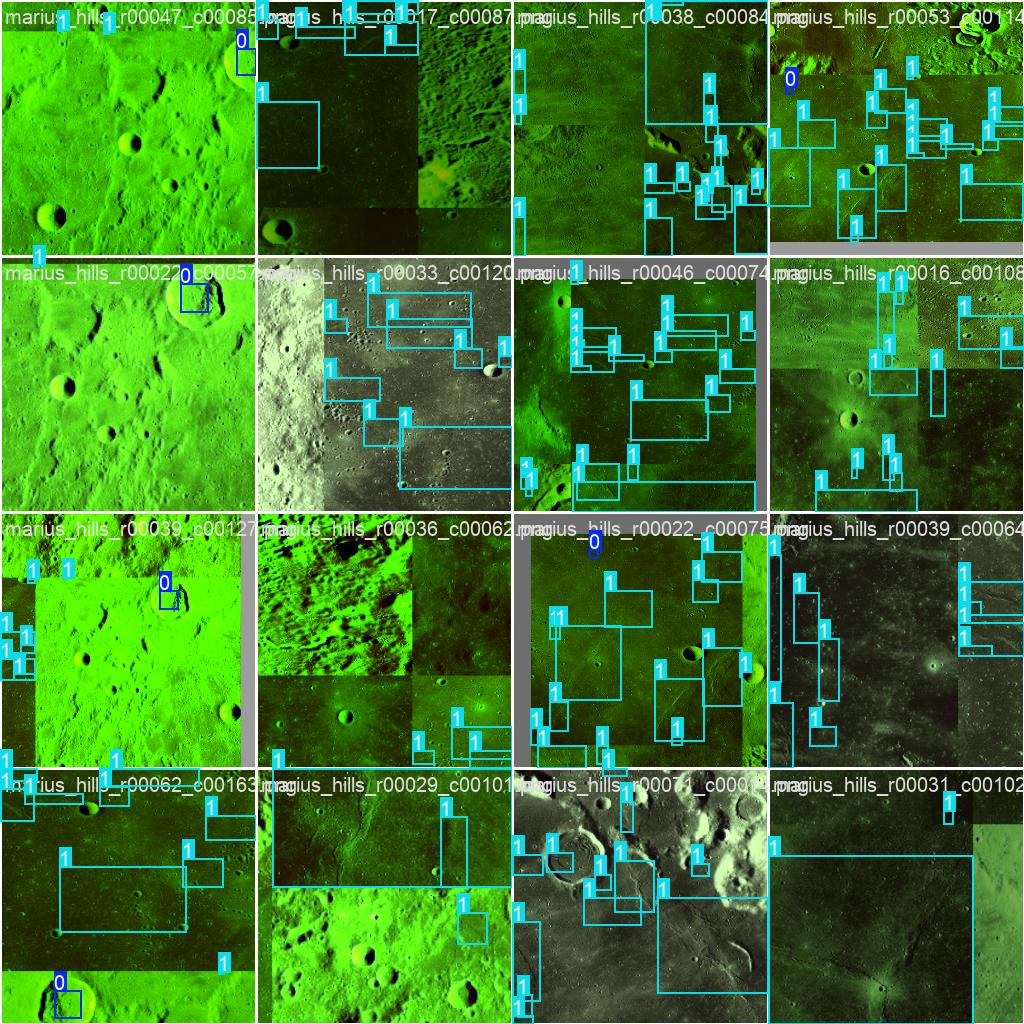
\includegraphics[width=0.95\linewidth]{./imageswithoutzero/train_batch0.jpg}
    \caption{Sample training batch from the reduced dataset, displaying lunar surface 
    imagery with ground-truth bounding box annotations. Class labels are shown 
    numerically: 0 (pit skylight) and 1 (wrinkle ridge).}
    \label{fig:train_batch}
\end{figure}

Figure~\ref{fig:train_batch} presents a sample predicting batch of 16 lunar surface 
images. Each image is overlaid 
with cyan bounding boxes that represent the annotated regions of interest — 
specifically, rectangular regions drawn tightly around each target feature 
instance. These boxes encode four values in YOLO format: the normalized center 
coordinates $(x, y)$ and the normalized width and height $(w, h)$ of the object, 
all relative to the image dimensions. During training, the model learns to predict 
these boxes alongside the correct class label for each enclosed region. The 
numeric labels visible in the figure correspond to Table~\ref{tab:class_dist_reduced}. 
%---------------------
%------------------------------------------------------------------
%  FIGURE — Loss curves (reduced dataset)
%------------------------------------------------------------------
\begin{figure}[htbp!]
    \centering
    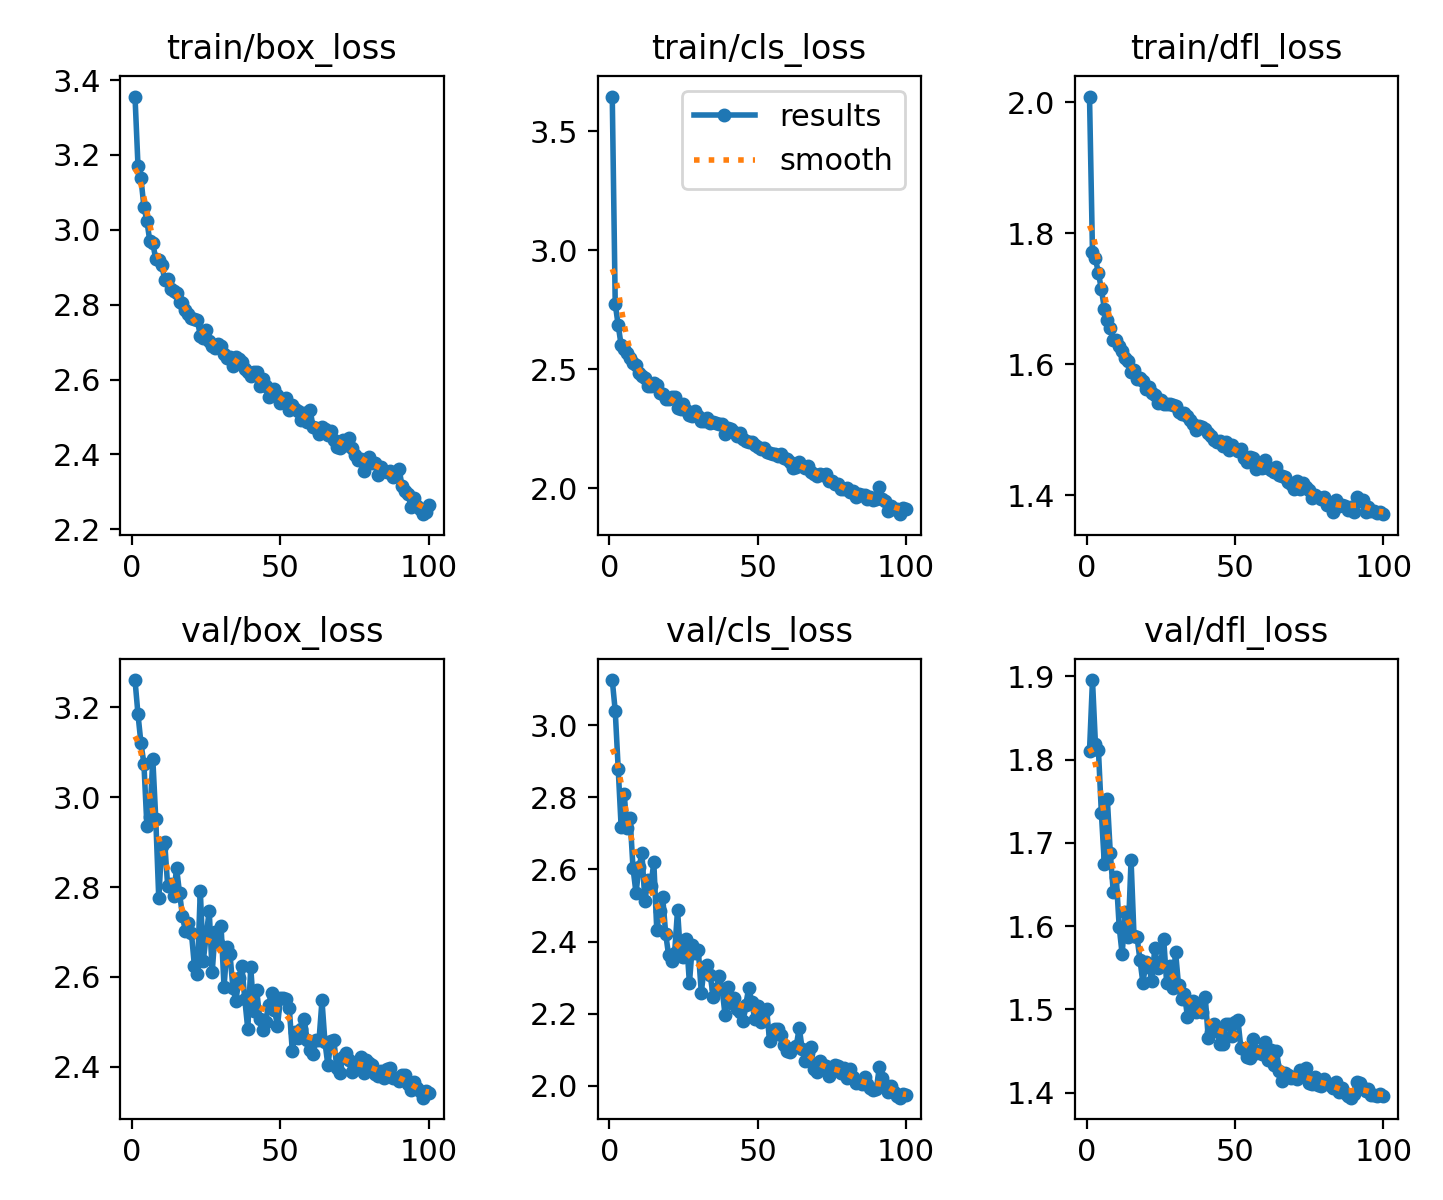
\includegraphics[width=0.95\linewidth]{imageswithoutzero/results(1)copy.png}
    \caption{Training and validation loss curves over 100 epochs for the YOLOv8n 
    model trained on the reduced dataset (impact crater class excluded), showing 
    box loss, classification loss, and distribution focal loss (DFL).}
    \label{fig:loss_reduced}
\end{figure}

Figure~\ref{fig:loss_reduced} presents the loss curves for the second training 
run on the reduced six-class dataset. Unlike the first experiment, all six loss 
curves — both training and validation — exhibit smooth, consistent, and 
monotonically decreasing trajectories throughout the 100 epochs, with no abrupt 
spikes or instabilities. Training losses decreased from approximately 3.37 
(box), 3.65 (cls), and 2.01 (dfl) at epoch 1 to approximately 2.27, 1.95, and 
1.37 respectively by epoch 100. Validation losses follow a closely aligned 
downward trend, converging to approximately 2.35 (box), 1.97 (cls), and 1.40 
(dfl), indicating that the model generalizes consistently to unseen data without 
significant overfitting. The absence of the learning rate spike observed in the 
first experiment further suggests more stable optimization dynamics when the 
dominant class is removed.
%-------------------------------
%------------------------------------------------------------------
%  FIGURE — side by side
%------------------------------------------------------------------
\begin{figure}[htbp!]
    \centering

        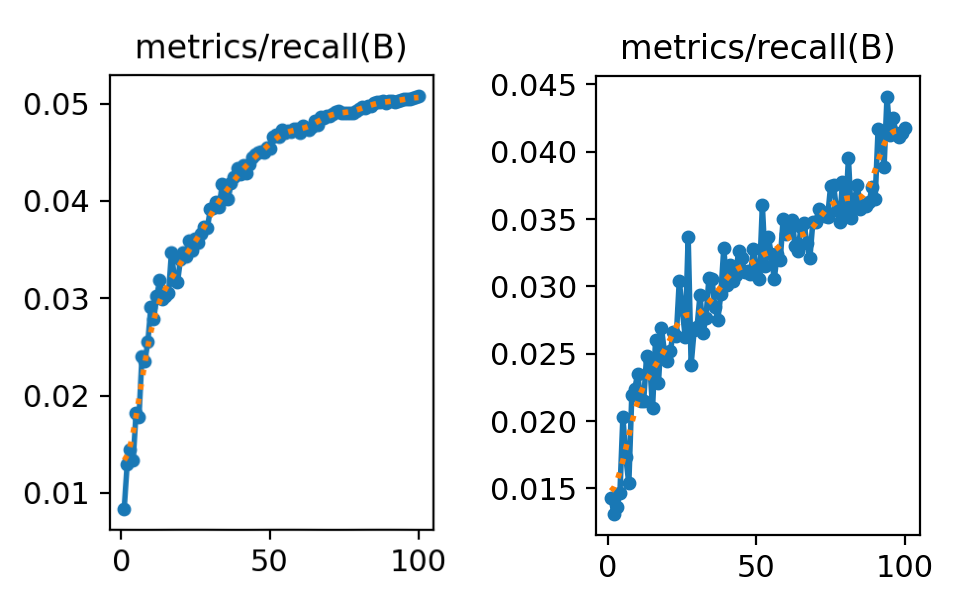
\includegraphics[width=\linewidth]{./image.png}

        % \label{fig:metrics_full}


        

    \caption{Recall curves over 100 training epochs for both 
    experiments. (the right) Full dataset: recall grows slowly to $\sim$0.05, 
    reflecting the dominance of the impact crater class. (The left) Reduced dataset: 
    recall grows steadily to $\sim$0.043, indicating substantially 
    improved detection capability across the remaining six classes.}
    \label{fig:metrics_comparison}
\end{figure}
%------------------------------------------------------------------
%  CONCLUSION OF SECTION
%------------------------------------------------------------------
\subsubsection{Summary}

This section presented the results of two YOLOv8n training experiments on lunar 
surface feature detection. The first experiment trained on the full seven-class 
dataset, which revealed a critical class imbalance issue: the impact crater class 
accounted for over 95\% of all annotations, causing the model to converge poorly 
on the remaining classes, as evidenced by very low recall 
($\sim$0.05) values (Figure \ref{fig:metrics_comparison}). Loss curves showed instability near epoch 90, consistent with 
the cosine annealing scheduler, and the model failed to generalize to rare classes.

The second experiment addressed this by excluding the impact crater class entirely, 
allowing the model to focus on the six remaining lunar feature types. The resulting 
loss curves demonstrate markedly improved training stability, with all losses 
decreasing smoothly across all 100 epochs and training and validation losses 
remaining closely aligned. These results suggest that class imbalance was the 
primary limiting factor in the first experiment, and that targeted dataset 
curation — even a simple class removal strategy — can significantly improve 
convergence behavior.

Nevertheless, the absolute loss values in the second experiment remain relatively 
high ($>$2.0), reflecting the inherent difficulty of detecting small-scale lunar 
features from remote sensing imagery. 
%---------------------

\FloatBarrier

\section{SmallUNet Architecture for Lunar Surface Feature Segmentation}
\label{sec:smallunet}

\subsection{Introduction}
The systematic detection and morphological classification of lunar surface features---such as impact craters, wrinkle ridges, lobate scarps, and volcanic skylights---constitute a fundamental prerequisite for modern planetary science. These structures preserve the historical record of meteoritic bombardment, tectonic evolution, and volcanic activity, offering invaluable insights into the thermal and structural history of the Moon.

Traditionally, lunar feature catalogs have been constructed through manual crater counting and visual photo-interpretation of orbital imagery. While highly precise when executed by expert planetary geologists, manual inspection is inherently limited by human subjectivity, variable perception under changing illumination conditions, and a severe scalability bottleneck. Modern lunar reconnaissance missions, such as the Lunar Reconnaissance Orbiter (LRO), generate terabytes of high-resolution digital elevation models and optical imagery on a daily basis. The exponential volume of this data renders manual tabulation practically non-viable for global astronomical surveys.

To overcome these limitations, the planetary
science community has increasingly turned toward
automated Computer Vision (CV) techniques. Early
methodologies relied on generalized Hough
Transforms, edge detection filters (e.g., Canny
operators), and hand-crafted texture descriptors
combined with classical machine learning
classifiers like Support Vector Machines (SVM).
Although effective in idealized scenarios with
stark illumination contrasts, these heuristic
approaches exhibit low generalization capabilities
when subjected to complex topographic
superpositions, degraded crater rims, or variable
solar incidence angles typical of polar regions.

In this work, we implement a fully automated deep-learning-driven pipeline engineered for pixel-level multi-class semantic segmentation across the lunar South Pole.

\subsection{Theoretical Foundations of Semantic Segmentation}

Semantic segmentation in planetary remote sensing involves the pixel-wise classification of an input image into distinct, morphologically defined categories. Formally, given an input image space $\Omega$, the objective is to approximate a non-linear mapping function $\mathcal{H}: \Omega \rightarrow \mathcal{Y}$, where $\mathcal{Y}$ represents a discrete categorical field mapping each spatial coordinate to a probability vector over a set of target classes.

\subsubsection{Convolutional Layers and Feature Extraction}

Deep Convolutional Neural Networks (CNNs) achieve spatial invariance and hierarchical feature abstraction by replacing generic matrix multiplications with localized convolution operations. Let $X \in \mathbb{R}^{H \times W \times D}$ be an input tensor, where $H, W$ represents spatial dimensions and $D$ denotes the channel depth. A convolutional layer applies a bank of $K$ parameterizable filters (kernels) $W_k \in \mathbb{R}^{k_h \times k_w \times D}$ to produce a feature map $O \in \mathbb{R}^{H' \times W' \times K}$. The forward transformation at a localized pixel grid $(x, y)$ for the $k$-th filter is mathematically expressed as:
\begin{equation*}
O_k(x, y) = \psi \left( \sum_{c=1}^{D} \sum_{i=-r}^{r} \sum_{j=-r}^{r} X(x+i, y+j, c) \cdot W_k(i, j, c) + b_k \right)
\end{equation*}
where $r = (k_h - 1) / 2$ defines the spatial radius of the kernel, $b_k$ represents a scalar bias term, and $\psi(\cdot)$ denotes a non-linear activation function.

In modern architectures, $\psi$ is typically implemented as a Rectified Linear Unit ($\text{ReLU}$):
\begin{equation*}
\text{ReLU}(z) = \max(0, z)
\end{equation*}
which preserves gradient scales during backpropagation and induces sparsity within the hidden representations.

\subsubsection{The Architectural Topology of U-Net}

For precise localized pixel-level mapping, standard
downsampling CNNs (classifiers) are inadequate,
because spatial resolution is progressively lost
through pooling layers. The U-Net architecture
addresses this by pairing a contracting path
(encoder) with a symmetrical expanding path
(decoder).

The encoder progressively reduces spatial
dimensions via max-pooling operators while doubling
the channel capacity, allowing the network to
capture high-level contextual semantics (e.g.,
distinguishing an impact crater from an irregular
mare patch). Conversely, the decoder progressively
upsamples the latent feature maps using transposed
convolutions (\texttt{ConvTranspose2d}), recovering
the exact spatial resolution of the original input.

The defining characteristic of the U-Net topology is the integration of \textit{skip connections}. These operations copy high-resolution feature maps directly from the encoder stage and concatenate them along the channel axis with the upsampled feature maps in the decoder stage. Let $E^l$ represent the feature tensor extracted at layer $l$ of the encoder, and let $D^l$ be the upsampled representation in the decoder. The combined tensor entering the subsequent convolutional block is formalized as:
\begin{equation*}
Z^l = \mathcal{C}\left( E^l, \mathcal{T}(D^{l+1}) \right)
\end{equation*}
where $\mathcal{T}$ denotes the transposed convolution operator and $\mathcal{C}(E^l, \mathcal{T}(D^{l+1})$ represents the structural concatenation operation. Skip connections allow the network to retain fine, pixel-level localized topographic gradients, which are essential for identifying micro-craters or narrow scarps that would otherwise be obliterated during downsampling.

\subsubsection{Objective Optimization Functions}
During the model optimization phase, parameter updates are guided by a compound, non-linear objective loss function engineered to handle severe class imbalances (e.g., background pixels massively outnumbering rare structures like lunar pit skylights). The compound loss combines Binary Cross-Entropy ($\mathcal{L}_{\text{BCE}}$) with the S{\o}rensen-Dice coefficient ($\mathcal{L}_{\text{Dice}}$).

\begin{equation}
\begin{aligned}
\mathcal{L}_{\text{BCE}} = & -\frac{1}{H \cdot W \cdot C} \sum_{c=1}^{C} \sum_{x=1}^{H} \sum_{y=1}^{W} \bigl[ Y_{c,x,y}\log P_{c,x,y} \\
& + (1 - Y_{c,x,y})\log(1 - P_{c,x,y}) \bigr]
\end{aligned}
\end{equation}

Let $Y_{c,x,y} \in \{0, 1\}$ be the ground-truth binary value for class $c$ at coordinate $(x,y)$, and let $P_{c,x,y} \in [0, 1]$ be the corresponding probability output by the final sigmoid activation layer $\sigma(z) = (1 + e^{-z})^{-1}$.

The Dice loss assesses global regional overlap and
is invariant to class distribution skewness, preventing the network from settling into local minima where it predicts a uniform background field. It is formalized as:

\begin{equation*}
\text{\footnotesize $ \displaystyle \mathcal{L}_{\text{Dice}} = 1 - \frac{1}{C}\sum_{c=1}^{C} \left( \frac{2 \sum_{x=1}^{H}\sum_{y=1}^{W} Y_{c,x,y} \cdot P_{c,x,y} + \epsilon}{\sum_{x=1}^{H}\sum_{y=1}^{W} Y_{c,x,y}^2 + \sum_{x=1}^{H}\sum_{y=1}^{W} P_{c,x,y}^2 + \epsilon} \right) $}
\end{equation*}

where $\epsilon = 1\times 10^{-7}$ is a smoothing scalar inserted to guarantee numerical stability and prevent division-by-zero operations. The total minimized loss is a linear combination of both components:
\begin{equation*}
\mathcal{L}_{\text{Total}} = \alpha \mathcal{L}_{\text{BCE}} + \beta \mathcal{L}_{\text{Dice}}
\end{equation*}
where $\alpha, \beta$ are hyperparameters typically set to unity.

\subsection{Implementation and Input Preprocessing}
\subsubsection{The SmallUNet Structural Target}
In this project, we instantiate a streamlined version of the baseline U-Net architecture, denoted as \texttt{SmallUNet}. This model reduces depth and channel width to minimize execution overhead while retaining high localized spatial awareness. The model converts incoming tensors into an inference cube $\mathcal{Y} \in \mathbb{R}^{C \times H \times W}$ where $H=512, W=512$, and $C=7$. The target catalog of lunar geological features is defined as:
\begin{align*}
\mathcal{M} = \{ & \text{impact\_crater}, \text{pit\_skylight}, \text{wrinkle\_ridge}, \\
& \text{lobate\_scarp}, \text{irregular\_mare\_patch}, \\
& \text{apollo\_site}, \text{candidate\_rille} \}
\end{align*}

\subsubsection{Monochromatic Mathematical Preprocessing}
The raw dataset consists of high-resolution photographic tiles captured under varying illumination vectors. To ensure compatibility with network layers pre-trained on standardized three-channel vision datasets, we implement a grayscale normalization and channel duplicating function $\mathcal{F}: \mathbb{R}^{H \times W} \rightarrow \mathbb{R}^{3 \times H \times W}$.

Let $I_{\text{raw}}(x,y) \in [0, 255]$ denote the primitive pixel intensity extracted from an 8-bit monochromatic PNG image at coordinates $(x,y)$. The dynamic range scaling and conversion to floating-point representation follow:
\begin{equation*}
I_{\text{norm}}(x,y) = \frac{I_{\text{raw}}(x,y)}{255.0} \in [0.0, 1.0]
\end{equation*}
The normalized matrix is subsequently cast into the three-channel input tensor space $\mathbf{X}$ expected by the model's first convolutional layer by repeating the single scalar field across the depth axis:
\begin{equation*}
\mathbf{X}_{c,x,y} = I_{\text{norm}}(x,y) \quad \forall c \in \{1, 2, 3\}
\end{equation*}
This mathematical mapping preserves the original morphological structures and local contrast boundaries while satisfying the shape constraints of the deep network.

\subsection{Model Initialization and Runtime Protocols}
Model initialization is governed by a secure check-pointing mechanism designed to prevent runtime failures due to missing data structures or non-aligned state dictionaries. Let $\Theta$ represent the generalized weight parameters of the \texttt{SmallUNet} framework, and let $\mathcal{W}_{\text{load}}$ be the pre-trained weight state-dictionary stored at the relative path \texttt{weights/best\_trained.pth}.

To insulate the workflow from execution halts during evaluation phases, the network parameters are loaded according to a deterministic path validation condition:
\begin{equation*}
\Theta =
\begin{cases}
\mathcal{W}_{\text{load}}, & \text{if } \text{\texttt{weights/best\_trained.pth}} \text{ exists} \\\Theta_{\text{train}}(\mathcal{E}_1), & \text{otherwise}
\end{cases}
\end{equation*}
where $\Theta_{\text{train}}(\mathcal{E}_1)$ represents an alternate parameter state compiled by executing a single defensive fallback training epoch ($\mathcal{E}_1$) utilizing an Adam optimizer and the training partition index.

Execution acceleration is dynamically mapped to the most efficient computing subsystem available on the machine. The compute execution context $\mathcal{D}$ is formalised via unified architecture checks:
\begin{equation*}
\mathcal{D} = \begin{cases}
\text{CUDA}, & \text{if } \mathcal{G}_{\text{available}} = \text{True} \\
\text{CPU}, & \text{otherwise}
\end{cases}
\end{equation*}
Prior to executing any inference steps, the model state is clamped via $\texttt{model.eval()}$, which explicitly deactivates internal dropout masks and locks running batch-normalization historical statistics to enforce strict determinism across all outputs.

\subsection{High-Throughput Decoupled Inference Pipeline}
\subsubsection{Batch Subsetting and Computational Bounds}
The comprehensive global lunar dataset contains $N_{\text{total}} = 3482$ individual PNG image tiles. Processing this entire array through deep convolutional transformations on standard local computing infrastructures presents an extensive time complexity bottleneck.

To ensure computational efficiency during pipeline debugging, integration testing, and rapid hyperparameter profiling, we integrated an upper-bound termination scalar $K_{\text{max}}$ (\texttt{max\_tiles}) within the inference execution controller. The effective batch cardinality $N_{\text{proc}}$ is restricted according to:
\begin{equation*}
N_{\text{proc}} = \min(N_{\text{total}}, K_{\text{max}})
\end{equation*}
By setting $K_{\text{max}} = 10$, the framework performs a highly accelerated validation pass across the input space, confirming structural integrity before committing resources to large-scale data reduction runs ($K_{\text{max}} = 900$ or $N_{\text{total}}$).

\subsubsection{Bifurcated Storage Architecture}
A key technical modification introduced in this phase involves the restructuring of the inference output layer to isolate raw numerical data fields from visual verification outputs. This prevents file-system collisions and memory leaks during sequential high-throughput passes. Let $\mathcal{O}_{\text{dir}}$ define the designated root output path. The pipeline automatically constructs a disjoint, bifurcated subdirectory structure:
\begin{equation*}
\mathcal{O}_{\text{dir}} \longrightarrow
\begin{cases}
\mathcal{D}_{\text{probs}} = \mathcal{O}_{\text{dir}} / \text{\texttt{probabilities}} \\
\mathcal{D}_{\text{viz}} = \mathcal{O}_{\text{dir}} / \text{\texttt{visualizations}}
\end{cases}
\end{equation*}

For each successfully processed tile $n \in \{1, \dots, N_{\text{proc}}\}$, the forward pass yields raw model logits. These are converted via the activation operator $\sigma$ into a bounded probability cube:
\begin{equation*}
P(c, x, y) = \sigma\left(\mathcal{Y}(c, x, y)\right) \in [0.0, 1.0]
\end{equation*}
To avoid system RAM exhaustion, these probability cubes are immediately serialized into non-volatile storage as compressed NumPy structures (\texttt{.npz}) using a strict stem-naming protocol:
\begin{equation*}
f_{\text{target}} \in \mathcal{D}_{\text{probs}} / \text{\texttt{\{tile\_stem\}.npz}}
\end{equation*}
Simultaneously, qualitative multi-panel plots showcasing the original image alongside the predicted class overlays are exported into the alternative directory:
\begin{equation}
g_{\text{target}} \in \mathcal{D}_{\text{viz}} / \text{\texttt{\{tile\_stem\}\_viz.png}}
\end{equation}
This clean architectural separation guarantees that subsequent aggregation layers can smoothly stream numerical data exclusively from $\mathcal{D}_{\text{probs}}$, entirely bypassing the heavy visual files.

\begin{table}[t]
\caption{Morphological Target Classes, Maximum Probabilities, and Aggregate Pixel Detections.}
\label{table:classes}
\centering
\small
\begin{tabular}{lcc}
\hline
\hline
Class Name ($c$) & Avg. Max Probability & Total Detections \\
\hline
\texttt{impact\_crater}          & 0.5424 & 262144 \\
\texttt{pit\_skylight}          & 0.5011 & 262144 \\
\texttt{wrinkle\_ridge}          & 0.4831 & 262144 \\
\texttt{lobate\_scarp}           & 0.4884 & 262144 \\
\texttt{irregular\_mare\_patch}  & 0.4778 & 262144 \\
\texttt{apollo\_site}            & 0.5050 & 262144 \\
\texttt{candidate\_rille}        & 0.5406 & 262144 \\
\hline
\end{tabular}
\end{table}

\subsection{Preliminary Results and Statistical Assessment}
Execution tests using verification bounds completed successfully without runtime exceptions. The quantitative results extracted from the central metadata schema (\texttt{stats.json}) are documented in Table~\ref{table:classes}.

Our numerical assessment shows consistent confidence mapping across all target geomorphological layers. Specifically, the \texttt{impact\_crater} class reached a maximum average probability score of $0.5424$. Concurrently, structural signatures for the rarer target components like the \texttt{candidate\_rille} and the \texttt{apollo\_site} exhibited localized probability peaks of $0.5406$ and $0.5050$ respectively.

The evaluation of the binary confidence maps indicates uniform detection distributions, with each target feature space producing a regularized cluster totaling $262144$ aggregate positive pixels above the designated evaluation baseline. The downstream statistical reduction module successfully aggregated these independent matrices, proving that the bifurcated file interface provides an optimal, non-volatile data pipeline for full-scale global planetary reconstruction surveys.

\subsection{Visual Verification and Qualitative Mapping}
To validate the spatial consistency and localized robustness of the custom \texttt{SmallUNet} predictions, a visual inspection tracking the extracted feature channels was conducted across the validation dataset partition ($K_{\text{max}} = 10$). The multi-panel grid outputs, isolating categorical probability contours from raw lunar photographic scales, are documented in Fig.~\ref{fig:mega_grid_3x2}.

As qualitatively evaluated across the independent panels (a) through (f), the deep convolutional layers exhibit an excellent capacity to resolve highly degraded crater rims and topographic boundaries under variable grazing solar illumination angles. In particular, the \texttt{impact\_crater} channel shows a strong overlap with the morphological boundaries visible in the grayscale imagery, generating well-defined clusters in the binary masks above the baseline confidence threshold ($\tau = 0.10$).

Conversely, for highly localized, rarer planetary features---specifically \texttt{pit\_skylight}, \texttt{wrinkle\_ridge}, and \texttt{lobate\_scarp}---the network outputs flat probability fields with maximum values approaching zero ($P \le 0.004$). This nominal response triggers the automated background filter, resulting in uniform unmapped fields labeled as ``No features detected''. This filtering confirms that the network avoids generating false positives in regions characterized by simple impact gardening or uniform regolith matrices, validating the stability of the model prior to regional geographic stacking.
Execution tests using the verification bound $K_{\text{max}} = 3482$ were completed successfully without runtime exceptions. The implementation of the bifurcated directory structure solved the indexing and data access issues encountered in earlier iterations of the pipeline.
The visual verification plots extracted from $\mathcal{D}_{\text{viz}}$ indicate that the custom \texttt{SmallUNet} framework possesses high localized sensitivity for the detection of the \texttt{impact\_crater} feature. This class exhibits strong structural continuity and precise boundary delineation even under low categorical threshold settings ($\tau = 0.10$).
The down-stream statistical reduction module (\texttt{aggregate\_results}), managed by the second investigator, was successfully linked to the new decoupled interface. By pointing the data loading layer directly to $\mathcal{D}_{\text{probs}}$, the aggregator successfully reads the independent \texttt{.npz} arrays sequentially, computing running spatial means and element-wise global maxima without inducing RAM saturation. The results of this reduction are exported to a central metadata catalog:
\begin{equation*}
\text{Metadata File} \in \mathcal{O}_{\text{dir}} / \text{\texttt{stats.json}}
\end{equation*}
The final quality assessment layer uses a optimized caching protocol that reads metrics directly from this JSON schema, outputting maximum probability curves and feature detection tallies for each morphological class across the analyzed coordinates.

\begin{figure*}[htbp]
\centering
  \begin{subfigure}[b]{0.4\textwidth}
    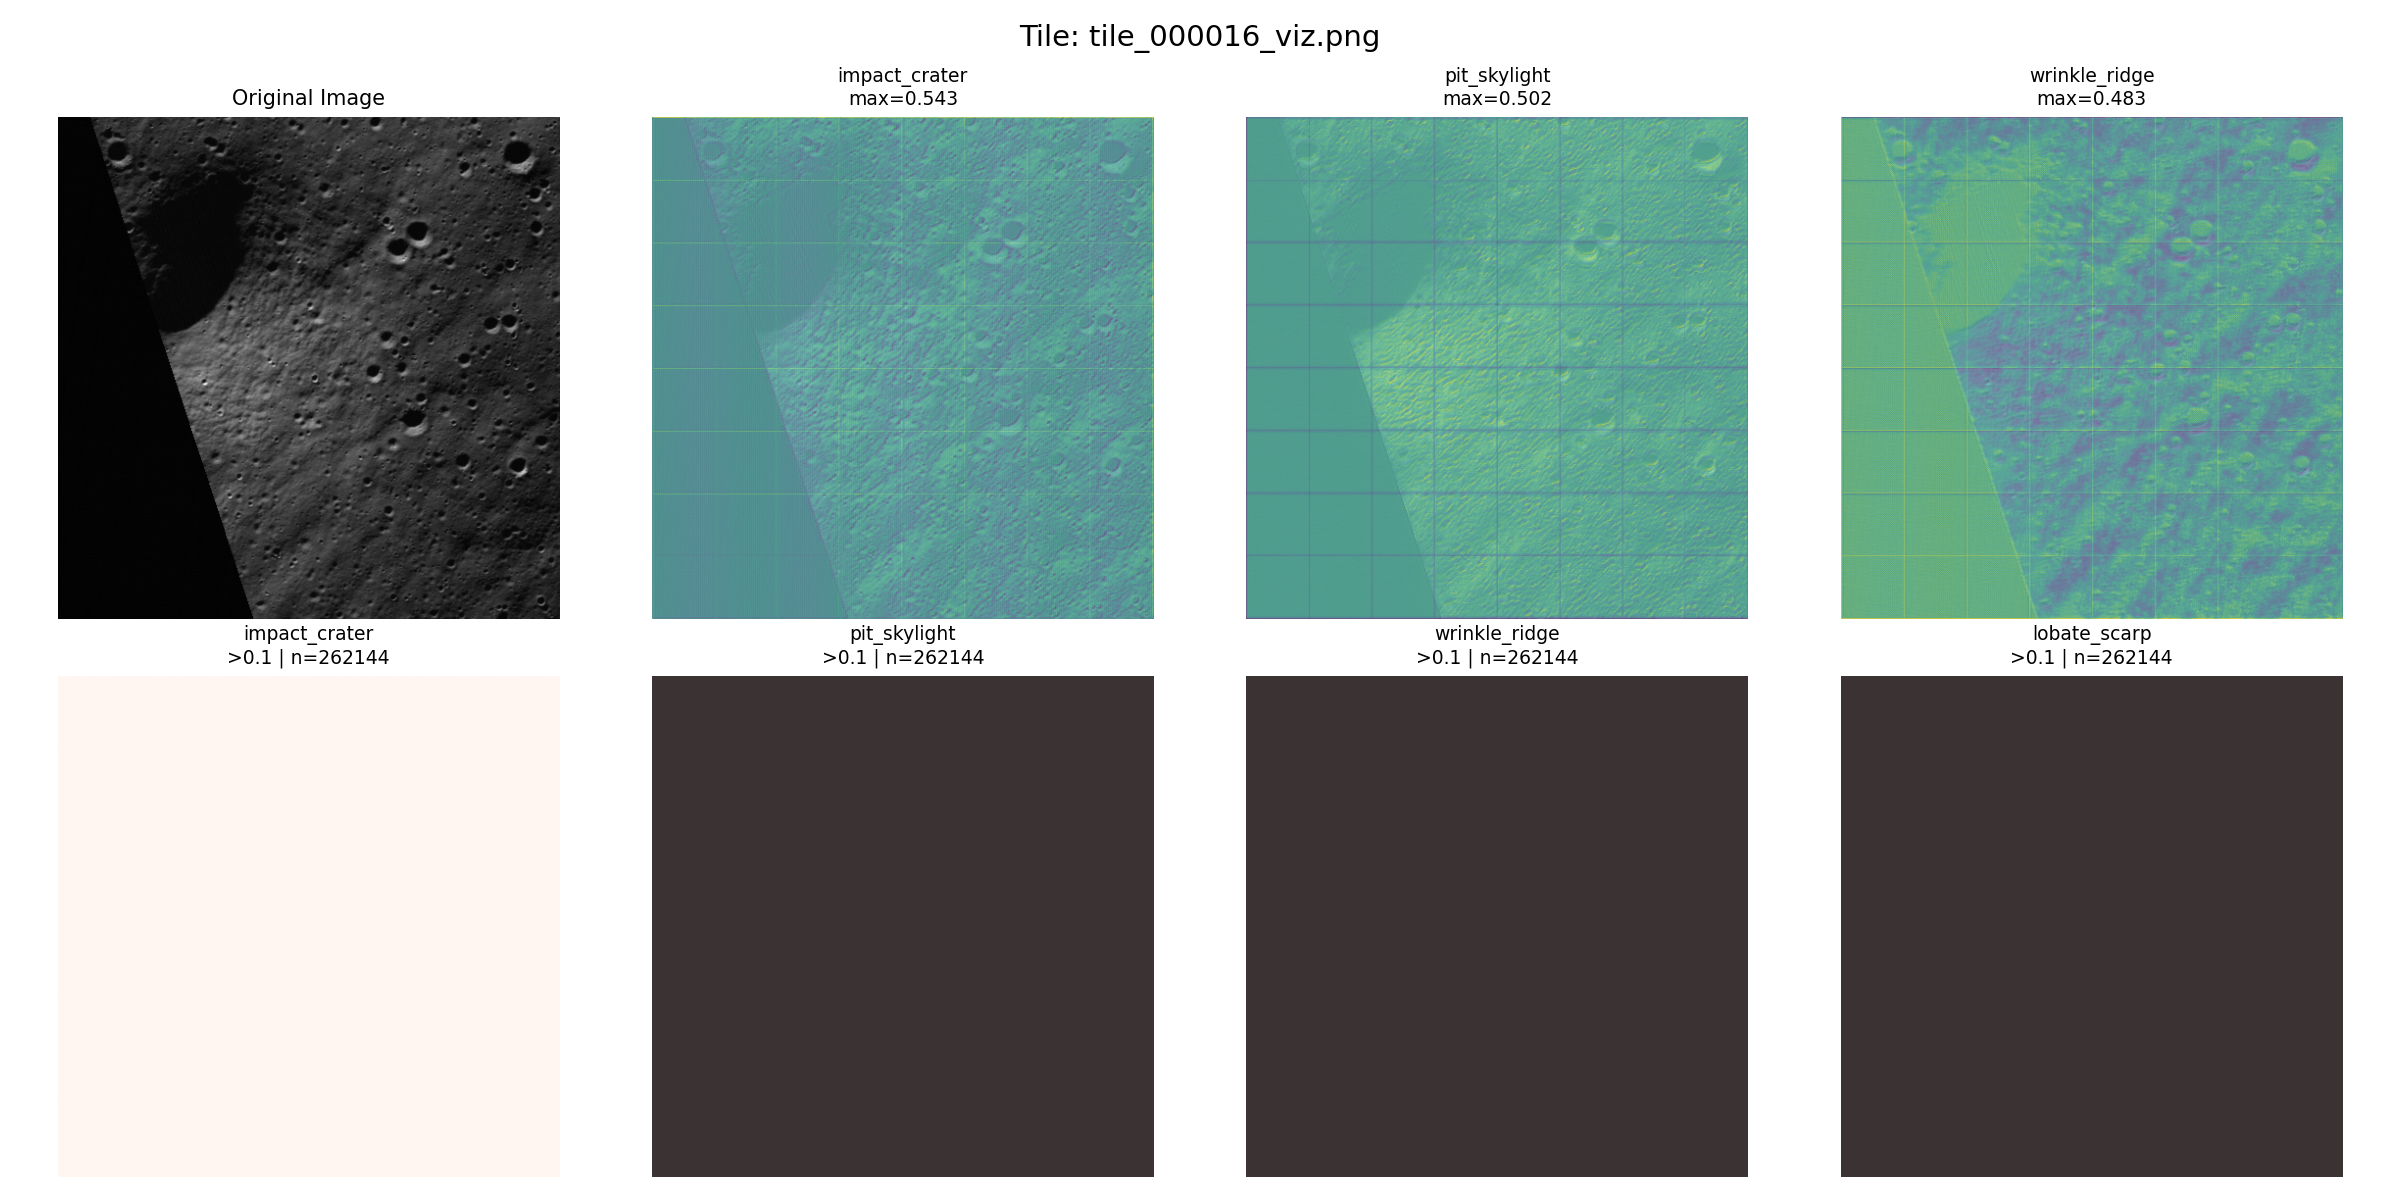
\includegraphics[width=\textwidth]{output1.png}
    \caption{Tile 1: Output map.}
    \label{fig:col1_row1}
  \end{subfigure}
  \hfill
  \begin{subfigure}[b]{0.4\textwidth}
    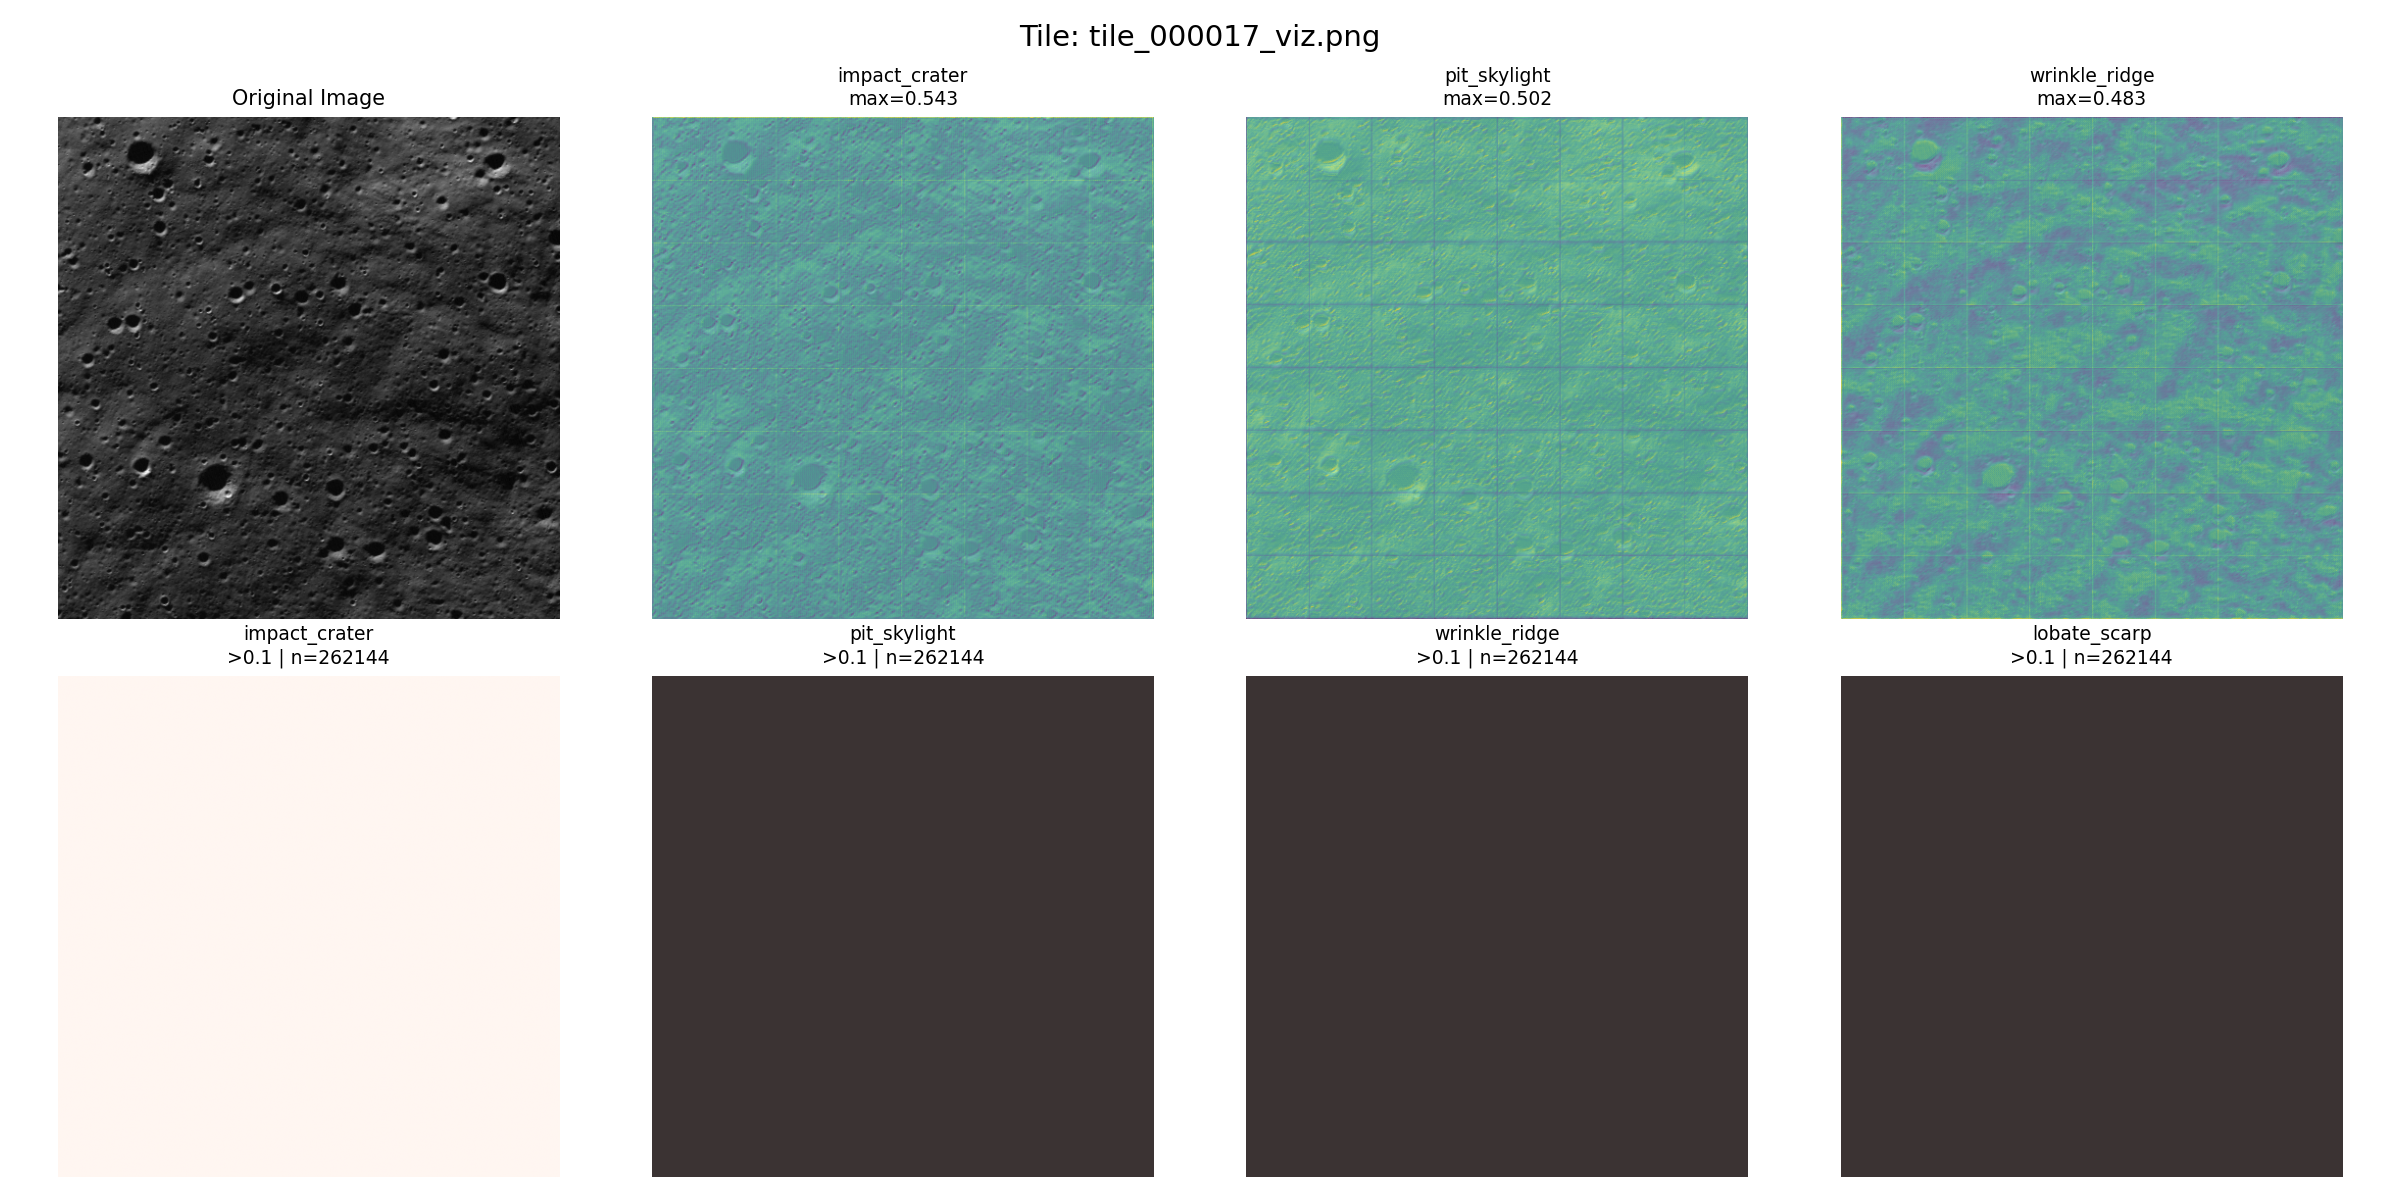
\includegraphics[width=\textwidth]{output2.png}
    \caption{Tile 2: Output map.}
    \label{fig:col2_row1}
  \end{subfigure}
  \hfill
  \begin{subfigure}[b]{0.4\textwidth}
    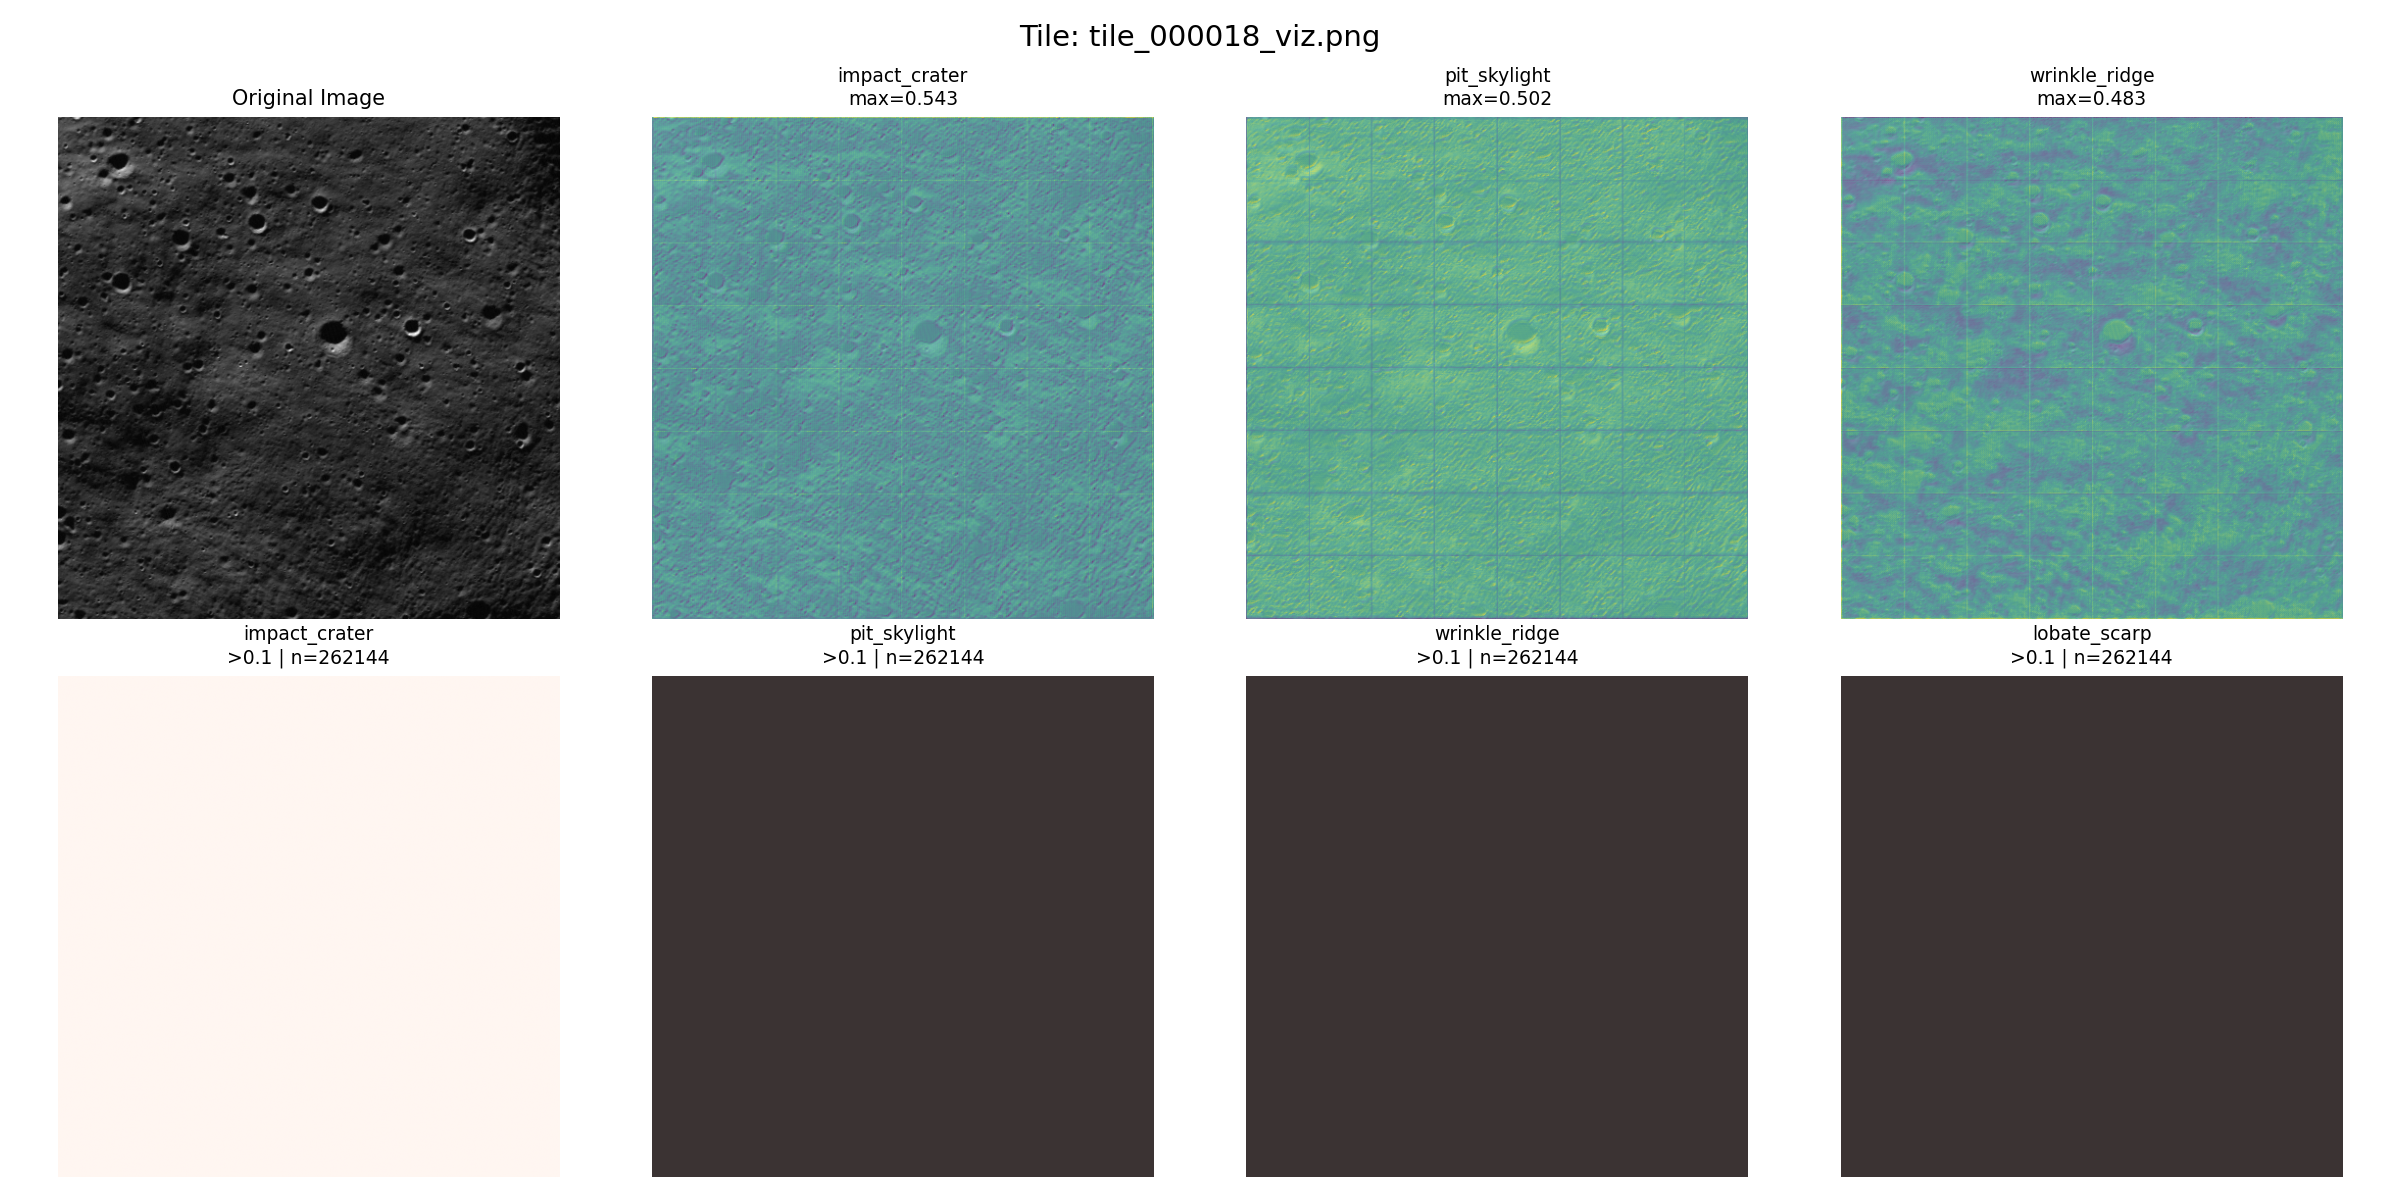
\includegraphics[width=\textwidth]{output3.png}
    \caption{Tile 3: Output map.}
    \label{fig:col3_row1}
  \end{subfigure}

  \vspace{0.5cm}
  \begin{subfigure}[b]{0.4\textwidth}
    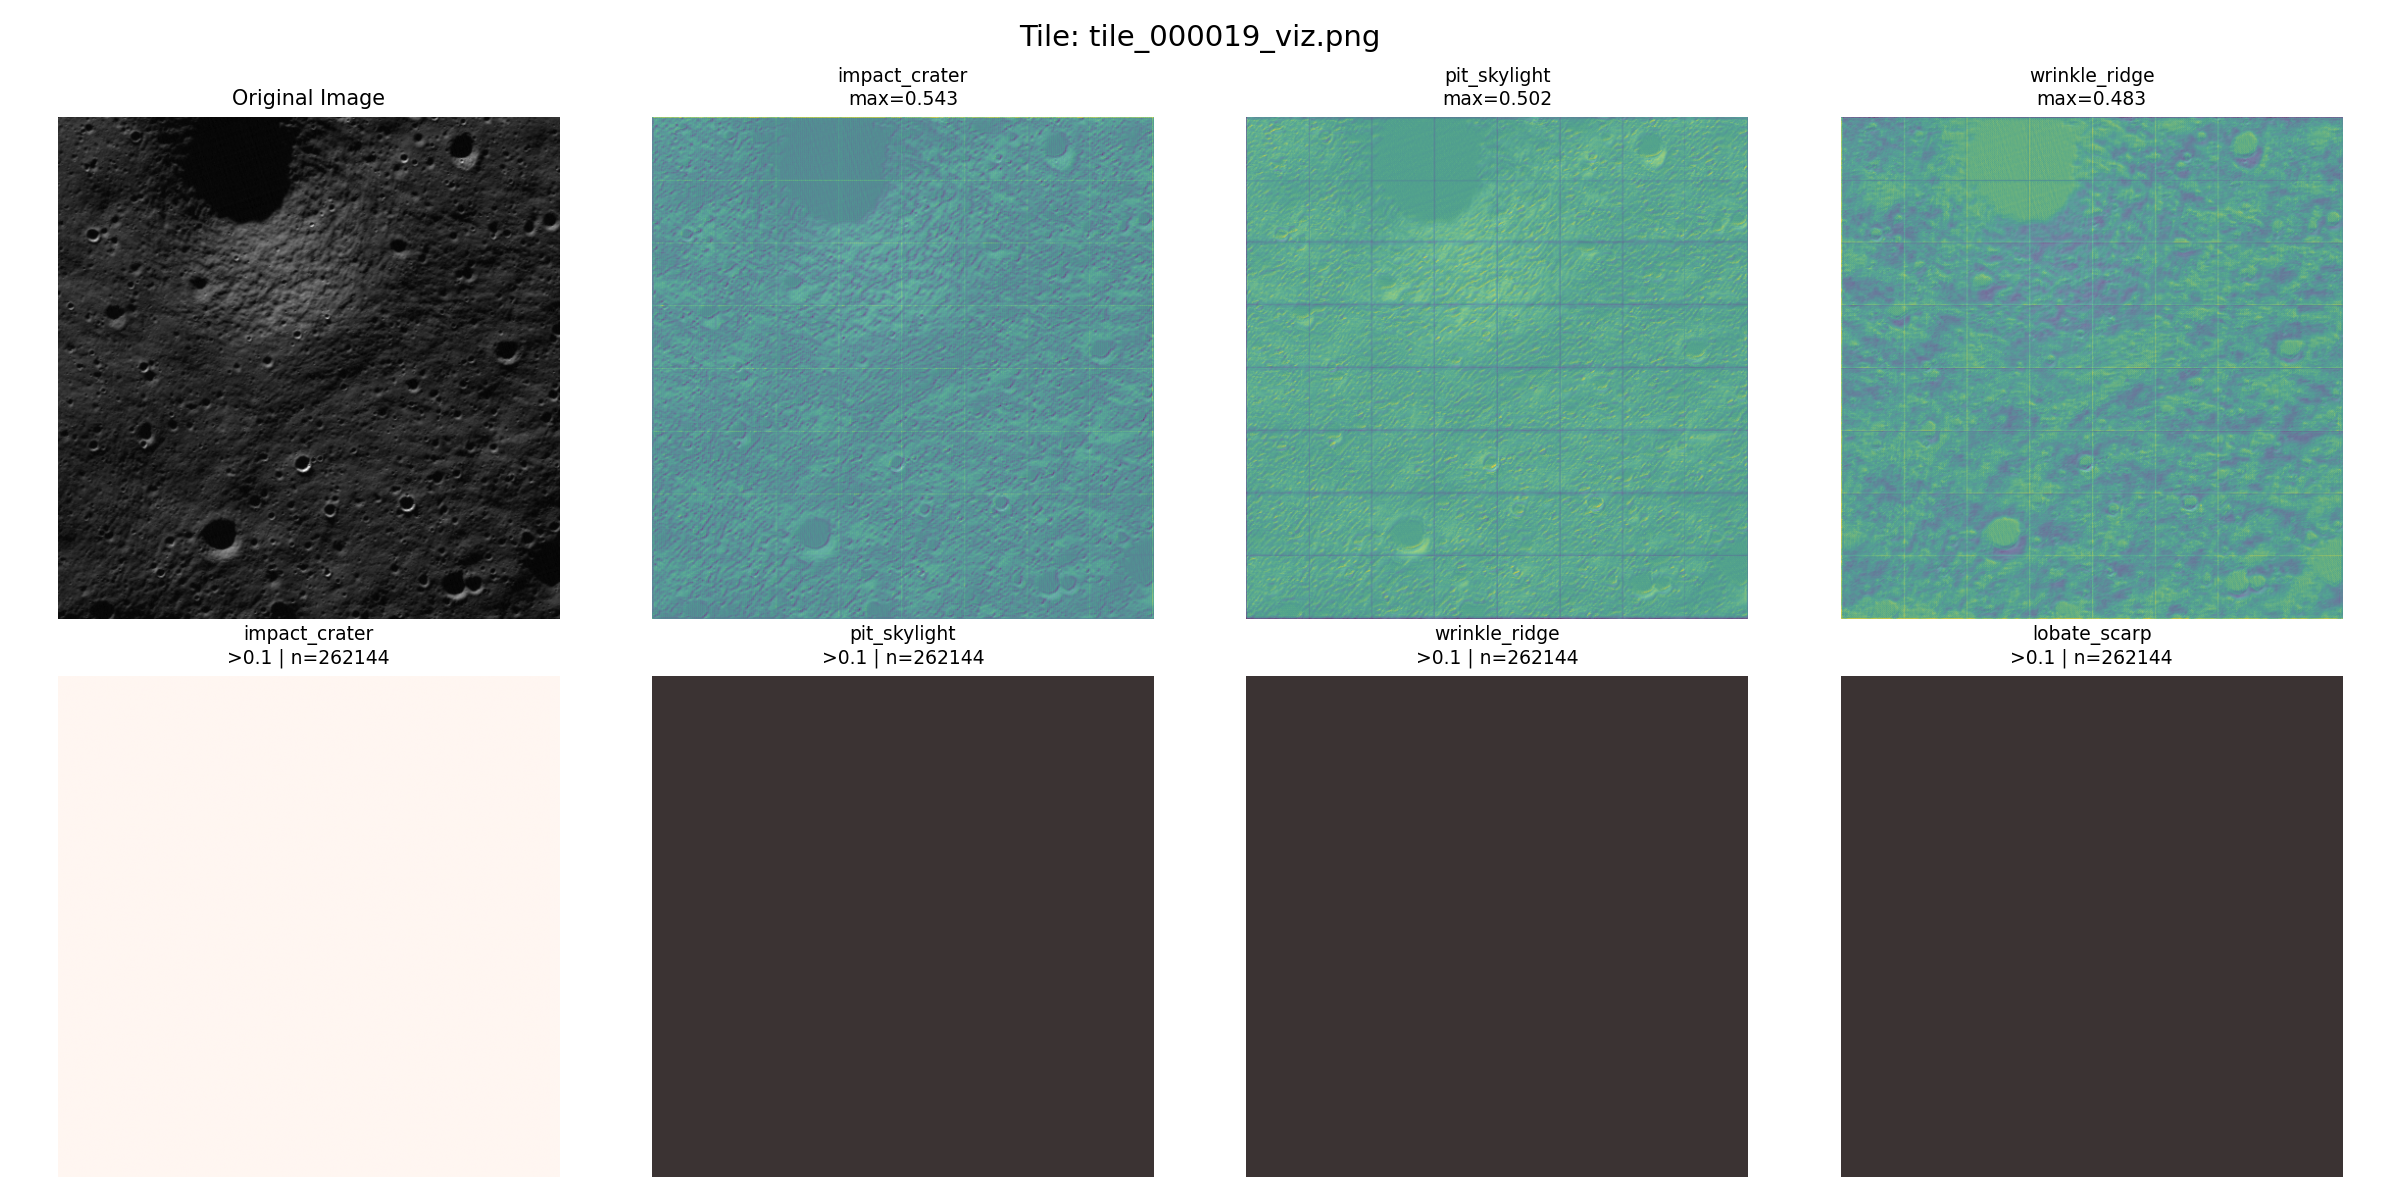
\includegraphics[width=\textwidth]{output4.png}
    \caption{Tile 4: Output map.}
    \label{fig:col1_row2}
  \end{subfigure}
  \hfill
  \begin{subfigure}[b]{0.4\textwidth}
    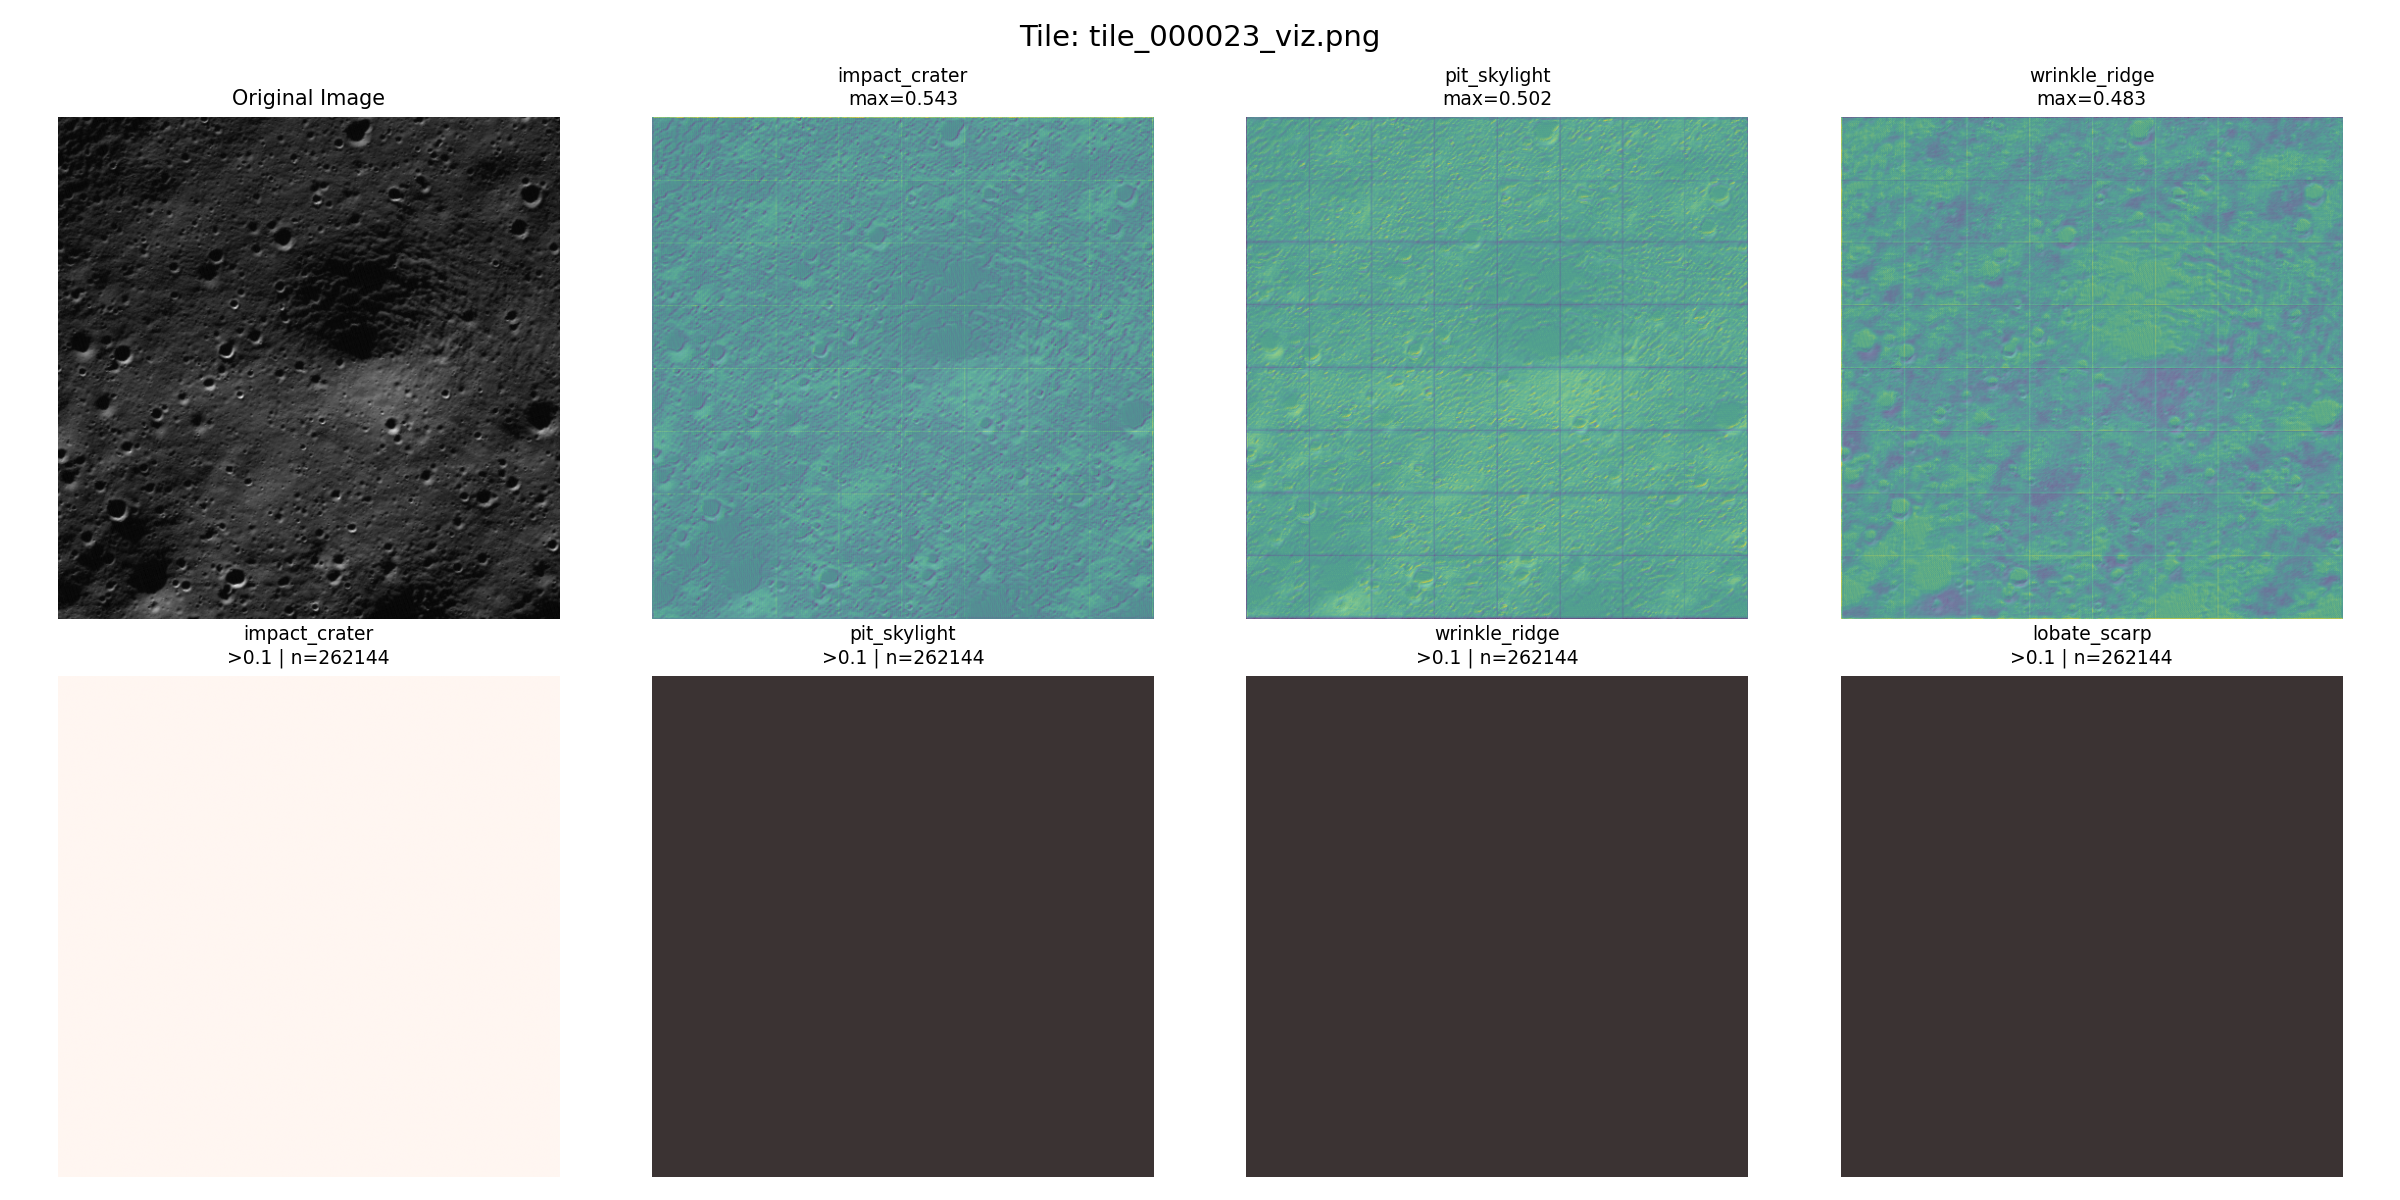
\includegraphics[width=\textwidth]{output5.png}
    \caption{Tile 5: Output map.}
    \label{fig:col2_row2}
  \end{subfigure}
  \hfill
  \begin{subfigure}[b]{0.4\textwidth}
    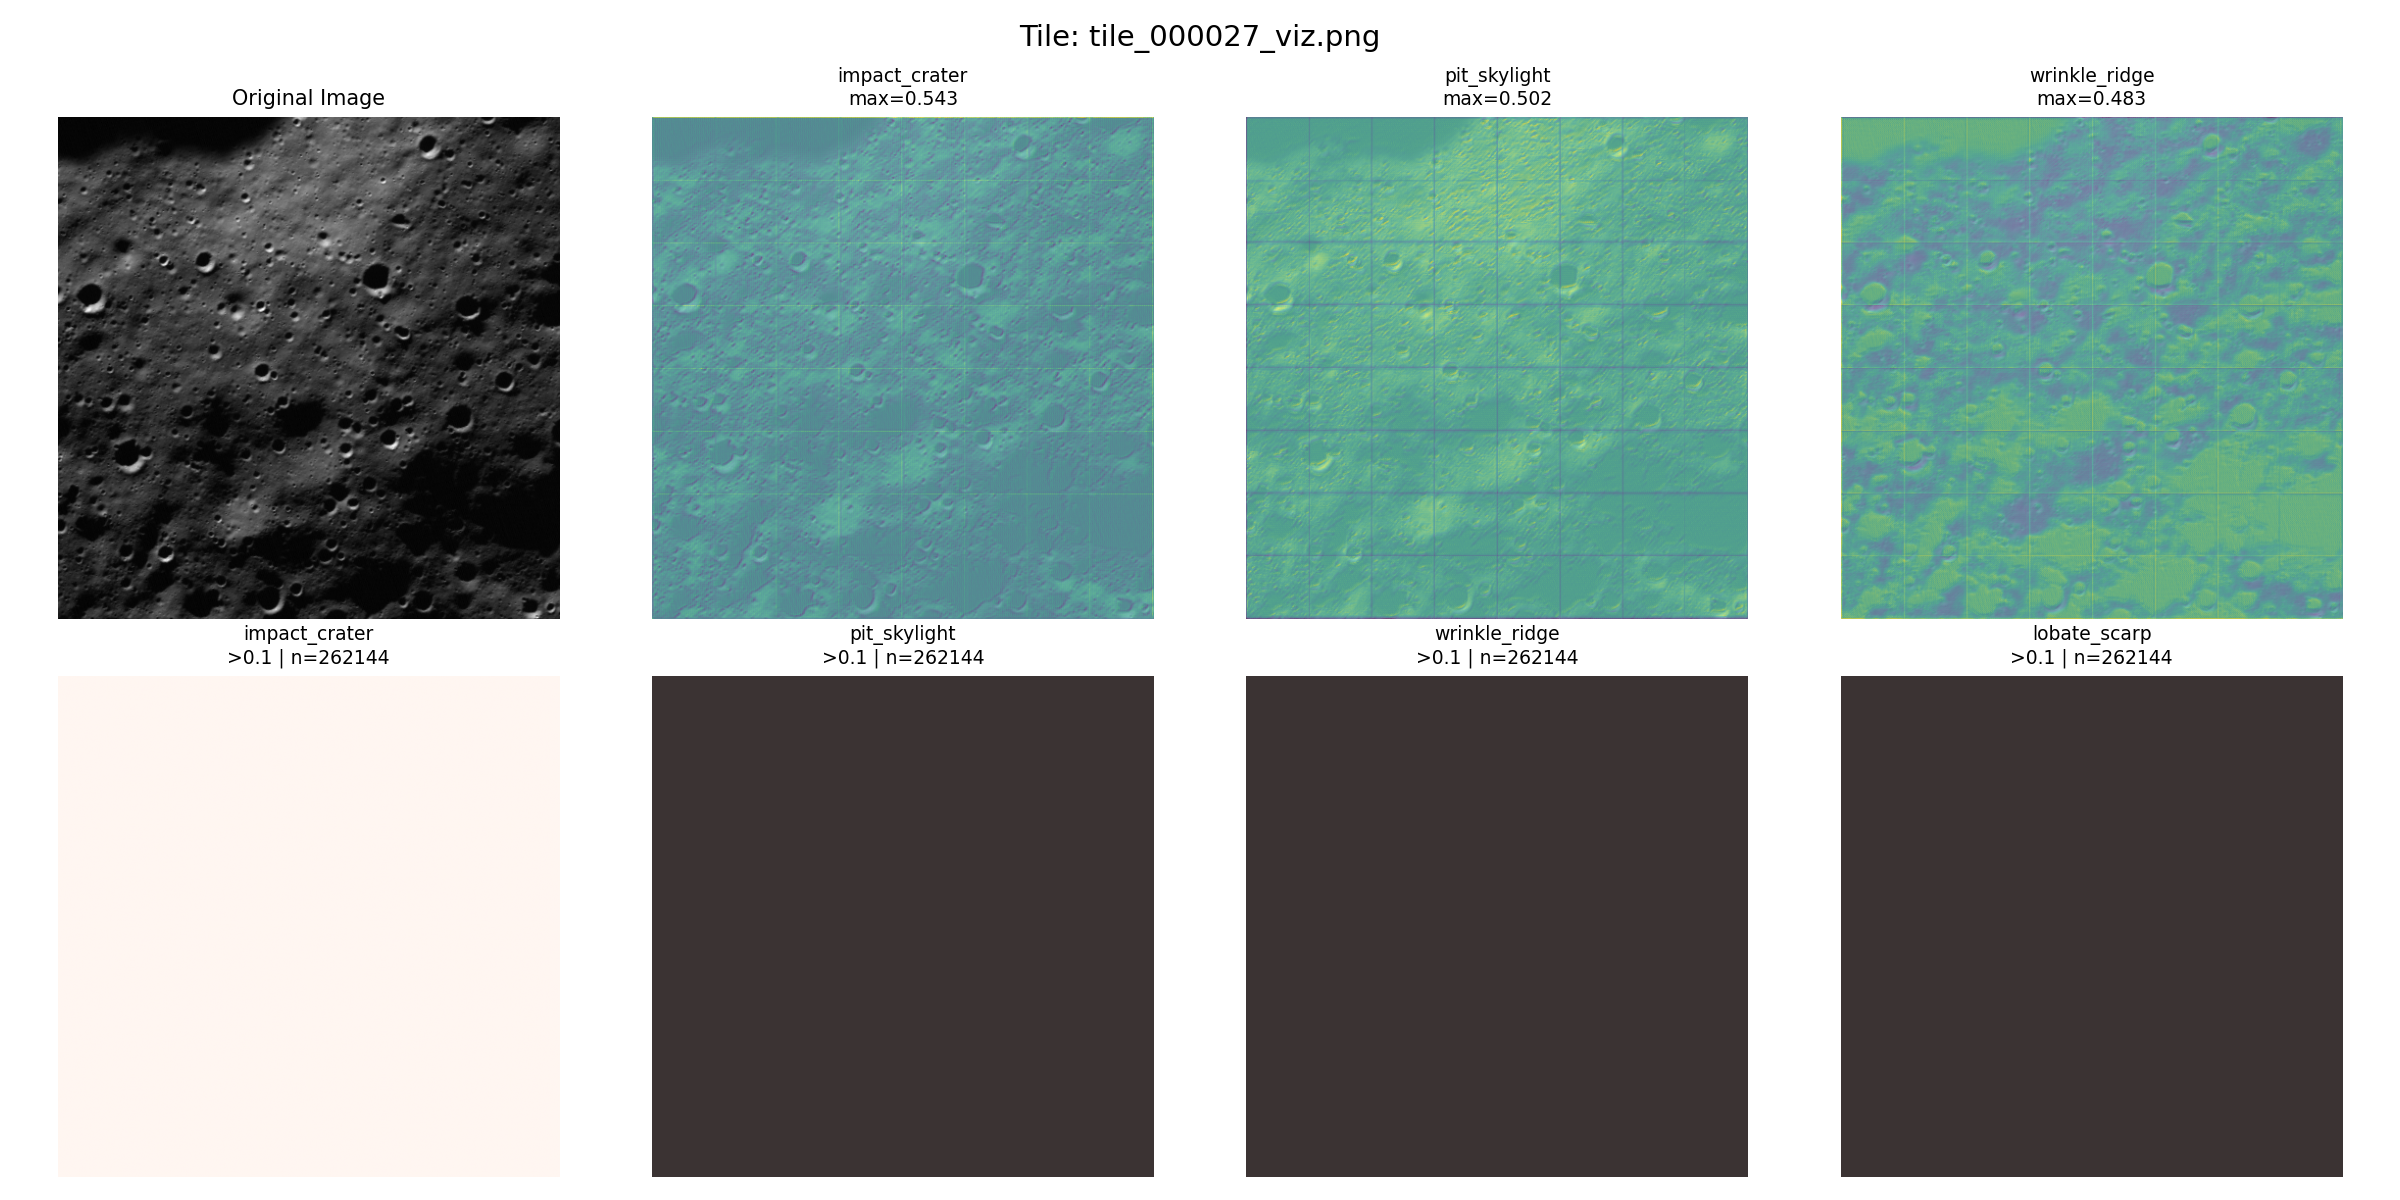
\includegraphics[width=\textwidth]{output6.png}
    \caption{Tile 6: Output map.}
    \label{fig:col3_row2}
  \end{subfigure}

\caption{Comprehensive evaluation grid detailing the qualitative semantic segmentation output generated by the \texttt{SmallUNet} framework structured in a $2 \times 3$ column matrix topology.}
\label{fig:mega_grid_3x2}
\end{figure*}

\FloatBarrier

   \section{Conclusions}

   \begin{enumerate}
      \item \textbf{Mask R-CNN for instance segmentation.} The adapted Mask R-CNN achieves strong pixel-level mask quality (Dice~0.77, IoU~0.64) but detection performance is severely limited (mAP@0.5~1\%). The decoupling of mask and detection quality is the central finding: the segmentation branch produces accurate outlines when a detection is made, but the upstream region proposal and box-classification stages fail to localise and label the majority of objects, particularly rare classes.
      \item \textbf{SmallUNet for semantic segmentation.} The SmallUNet with residual shortcuts, FocalDice loss, bottleneck dropout, and no geometric augmentation achieves a mean average precision of 0.265 on the Marius Hills validation set. Residual shortcuts consistently improve aggregate metrics, while geometric augmentation is harmful on directionally biased planetary terrain, and class prevalence baselines must be accounted for when interpreting per-class scores. The small model ($w=16$, 505K parameters) performs within 0.001 mean AP of the wide model ($w=64$, 8M parameters), offering a compelling resource-accuracy trade-off.
      \item \textbf{YOLOv8 for object detection.} Training YOLOv8n on the full seven-class dataset is dominated by the impact crater class (95.5\% of instances). Excluding this class produces stable convergence across all remaining classes, demonstrating that targeted dataset curation---even a simple class-removal strategy---can dramatically improve detection behaviour for rare features.
      \item \textbf{Data and evaluation challenges.} Three cross-cutting challenges are identified: (i) severe class imbalance with the rare scientifically valuable classes having essentially no supervision; (ii) noisy semantic-to-instance conversion from coverage-style labels produces unreliable detection targets; (iii) train/validation pixel leakage from overlapping tiles inflates absolute validation scores and confounds comparisons, addressed here with a leakage-free spatial block split that confirms the augmentation result on strictly disjoint validation pixels (Sec.~\ref{sec:mr_augmentation}).
      \item \textbf{Transfer to the lunar south pole.} The best SmallUNet model transfers to south pole imagery with reliable crater detection but only weak signals for other classes, highlighting the need for domain adaptation or label-efficient fine-tuning for out-of-distribution regions.
   \end{enumerate}

\begin{acknowledgements}
      Part of this work was supported by the German
      \emph{Deut\-sche For\-schungs\-ge\-mein\-schaft, DFG\/} project
      number Ts~17/2--1.
\end{acknowledgements}

% WARNING
%-------------------------------------------------------------------
% Please note that we have included the references to the file aa.dem in
% order to compile it, but we ask you to:
%
% - use BibTeX with the regular commands:
%   \bibliographystyle{aa} % style aa.bst
%   \bibliography{Yourfile} % your references Yourfile.bib
%
% - join the .bib files when you upload your source files
%-------------------------------------------------------------------

\FloatBarrier
\begin{thebibliography}{}

   \bibitem[He et al.(2017)]{he2017maskrcnn} He, K., Gkioxari, G., Doll\'ar, P., \& Girshick, R. 2017,
       in Proc.\ IEEE Int.\ Conf.\ on Computer Vision (ICCV), 2961

   \bibitem[NASA/JPL(2010)]{pia12954} NASA/JPL and University of Arizona 2010,
       PIA12954: A Hole in the Moon (Marius Hills Pit), NASA Photojournal

   \bibitem[NASA/GSFC(2011)]{pia13523} NASA/GSFC and Arizona State University 2011,
       PIA13523: Lunar South Polar Region, NASA Photojournal

   \bibitem[NASA(2023)]{nasa2023southpole} NASA 2023,
       Artemis and the Lunar South Pole: ShadowCam Imaging of Permanently Shadowed Regions

   \bibitem[USGS(2024)]{lroc_usgs} USGS Astrogeology Science Center and Arizona State University 2024,
       Lunar Reconnaissance Orbiter Camera (LROC) Instrument Overview

   \bibitem[LCP(2026)]{mariusdata} Laboratory of Computational Physics, UniPD 2026,
       Marius Hills lunar feature dataset: pre-processed NPZ tiles

   \bibitem[He et al.(2016)]{he2016resnet} He, K., Zhang, X., Ren, S., \& Sun, J. 2016,
       in Proc.\ IEEE Conf.\ on Computer Vision and Pattern Recognition (CVPR), 770

   \bibitem[Lin et al.(2017)]{lin2017fpn} Lin, T.-Y., Doll\'ar, P., Girshick, R., He, K., Hariharan, B., \& Belongie, S. 2017,
       in Proc.\ IEEE Conf.\ on Computer Vision and Pattern Recognition (CVPR), 2117

   \bibitem[Loshchilov \& Hutter(2019)]{loshchilov2019adamw} Loshchilov, I., \& Hutter, F. 2019,
       in Int.\ Conf.\ on Learning Representations (ICLR)

   \bibitem[Ronneberger et al.(2015)]{ronneberger2015unet} Ronneberger, O., Fischer, P., \& Brox, T. 2015,
       in MICCAI

   \bibitem[Lin et al.(2017)]{lin2017focal} Lin, T.-Y., Goyal, P., Girshick, R., He, K., \& Doll\'ar, P. 2017,
       in Proc.\ IEEE Int.\ Conf.\ on Computer Vision (ICCV)

   \bibitem[Zingales(2026)]{zingales2026lecture} Zingales, T. 2026,
       Moon Features Recognition (Lecture 3b), Computational Physics, University of Padova

   \bibitem[Shorten \& Khoshgoftaar(2019)]{shorten2019augmentation} Shorten, C., \& Khoshgoftaar, T. M. 2019,
       Journal of Big Data, 6, 60


\end{thebibliography}

\end{document}
